%%%%%%%%%%%%%%%%%%%%%%%%%%%%%%%%%%%%%%%%%
% The Legrand Orange Book
% LaTeX Template
% Version 2.4 (26/09/2018)
%
% This template was downloaded from:
% http://www.LaTeXTemplates.com
%
% Original author:
% Mathias Legrand (legrand.mathias@gmail.com) with modifications by:
% Vel (vel@latextemplates.com)
%
% License:
% CC BY-NC-SA 3.0 (http://creativecommons.org/licenses/by-nc-sa/3.0/)
%
% Compiling this template:
% This template uses biber for its bibliography and makeindex for its index.
% When you first open the template, compile it from the command line with the
% commands below to make sure your LaTeX distribution is configured correctly:
%
% 1) pdflatex main
% 2) makeindex main.idx -s StyleInd.ist
% 3) biber main
% 4) pdflatex main x 2
%
% After this, when you wish to update the bibliography/index use the appropriate
% command above and make sure to compile with pdflatex several times
% afterwards to propagate your changes to the document.
%
% This template also uses a number of packages which may need to be
% updated to the newest versions for the template to compile. It is strongly
% recommended you update your LaTeX distribution if you have any
% compilation errors.
%
% Important note:
% Chapter heading images should have a 2:1 width:height ratio,
% e.g. 920px width and 460px height.
%
%%%%%%%%%%%%%%%%%%%%%%%%%%%%%%%%%%%%%%%%%

%----------------------------------------------------------------------------------------
%	PACKAGES AND OTHER DOCUMENT CONFIGURATIONS
%----------------------------------------------------------------------------------------

\documentclass[11pt,fleqn]{book} % Default font size and left-justified equations

%%%%%%%%%%%%%%%%%%%%%%%%%%%%%%%%%%%%%%%%%
% The Legrand Orange Book
% Structural Definitions File
% Version 2.1 (26/09/2018)
%
% Original author:
% Mathias Legrand (legrand.mathias@gmail.com) with modifications by:
% Vel (vel@latextemplates.com)
%
% This file was downloaded from:
% http://www.LaTeXTemplates.com
%
% License:
% CC BY-NC-SA 3.0 (http://creativecommons.org/licenses/by-nc-sa/3.0/)
%
%%%%%%%%%%%%%%%%%%%%%%%%%%%%%%%%%%%%%%%%%

%----------------------------------------------------------------------------------------
%	VARIOUS REQUIRED PACKAGES AND CONFIGURATIONS
%----------------------------------------------------------------------------------------

\usepackage{graphicx} % Required for including pictures
\graphicspath{{Pictures/}} % Specifies the directory where pictures are stored

\usepackage{lipsum} % Inserts dummy text

\usepackage{tikz} % Required for drawing custom shapes
\newcommand*{\ClipSep}{0.3cm}%

\usepackage[portuguese]{babel} % English language/hyphenation

\usepackage{enumitem} % Customize lists
\setlist{nolistsep} % Reduce spacing between bullet points and numbered lists

\usepackage{booktabs} % Required for nicer horizontal rules in tables

\usepackage{xcolor} % Required for specifying colors by name
%\definecolor{ocre}{RGB}{243,102,25} % Define the orange color used for highlighting throughout the book
\definecolor{ocre}{RGB}{49,130,206} % Define the blue color used for highlighting throughout the book

%----------------------------------------------------------------------------------------
%	MARGINS
%----------------------------------------------------------------------------------------

\usepackage{geometry} % Required for adjusting page dimensions and margins

\geometry{
	paper=a4paper, % Paper size, change to letterpaper for US letter size
	top=3cm, % Top margin
	bottom=3cm, % Bottom margin
	left=3cm, % Left margin
	right=3cm, % Right margin
	headheight=14pt, % Header height
	footskip=1.4cm, % Space from the bottom margin to the baseline of the footer
	headsep=10pt, % Space from the top margin to the baseline of the header
	%showframe, % Uncomment to show how the type block is set on the page
}

%----------------------------------------------------------------------------------------
%	FONTS
%----------------------------------------------------------------------------------------

\usepackage{avant} % Use the Avantgarde font for headings
%\usepackage{times} % Use the Times font for headings
\usepackage{mathptmx} % Use the Adobe Times Roman as the default text font together with math symbols from the Sym­bol, Chancery and Com­puter Modern fonts

\usepackage{microtype} % Slightly tweak font spacing for aesthetics
\usepackage[utf8]{inputenc} % Required for including letters with accents
\usepackage[T1]{fontenc} % Use 8-bit encoding that has 256 glyphs

%----------------------------------------------------------------------------------------
%	BIBLIOGRAPHY AND INDEX
%----------------------------------------------------------------------------------------

\usepackage[style=numeric,citestyle=numeric,sorting=nyt,sortcites=true,autopunct=true,babel=hyphen,hyperref=true,abbreviate=false,backref=true,backend=biber]{biblatex}
\addbibresource{bibliography.bib} % BibTeX bibliography file
\defbibheading{bibempty}{}

\usepackage{calc} % For simpler calculation - used for spacing the index letter headings correctly
\usepackage{makeidx} % Required to make an index
\makeindex % Tells LaTeX to create the files required for indexing

%----------------------------------------------------------------------------------------
%	MAIN TABLE OF CONTENTS
%----------------------------------------------------------------------------------------
\setcounter{tocdepth}{1}
\usepackage{titletoc} % Required for manipulating the table of contents

\contentsmargin{0cm} % Removes the default margin

% Part text styling (this is mostly taken care of in the PART HEADINGS section of this file)
\titlecontents{part}
	[0cm] % Left indentation
	{\addvspace{20pt}\bfseries} % Spacing and font options for parts
	{}
	{}
	{}

% Chapter text styling
\titlecontents{chapter}
	[1.25cm] % Left indentation
	{\addvspace{12pt}\large\sffamily\bfseries} % Spacing and font options for chapters
	{\color{ocre!60}\contentslabel[\Large\thecontentslabel]{1.25cm}\color{ocre}} % Formatting of numbered sections of this type
	{\color{ocre}} % Formatting of numberless sections of this type
	{\color{ocre!60}\normalsize\;\titlerule*[.5pc]{.}\;\thecontentspage} % Formatting of the filler to the right of the heading and the page number

% Section text styling
\titlecontents{section}
	[1.25cm] % Left indentation
	{\addvspace{3pt}\sffamily\bfseries} % Spacing and font options for sections
	{\contentslabel[\thecontentslabel]{1.25cm}} % Formatting of numbered sections of this type
	{} % Formatting of numberless sections of this type
	{\hfill\color{black}\thecontentspage} % Formatting of the filler to the right of the heading and the page number

% Subsection text styling
\titlecontents{subsection}
	[1.25cm] % Left indentation
	{\addvspace{1pt}\sffamily\small} % Spacing and font options for subsections
	{\contentslabel[\thecontentslabel]{1.25cm}} % Formatting of numbered sections of this type
	{} % Formatting of numberless sections of this type
	{\ \titlerule*[.5pc]{.}\;\thecontentspage} % Formatting of the filler to the right of the heading and the page number

% Figure text styling
\titlecontents{figure}
	[1.25cm] % Left indentation
	{\addvspace{1pt}\sffamily\small} % Spacing and font options for figures
	{\thecontentslabel\hspace*{1em}} % Formatting of numbered sections of this type
	{} % Formatting of numberless sections of this type
	{\ \titlerule*[.5pc]{.}\;\thecontentspage} % Formatting of the filler to the right of the heading and the page number

% Table text styling
\titlecontents{table}
	[1.25cm] % Left indentation
	{\addvspace{1pt}\sffamily\small} % Spacing and font options for tables
	{\thecontentslabel\hspace*{1em}} % Formatting of numbered sections of this type
	{} % Formatting of numberless sections of this type
	{\ \titlerule*[.5pc]{.}\;\thecontentspage} % Formatting of the filler to the right of the heading and the page number

%----------------------------------------------------------------------------------------
%	MINI TABLE OF CONTENTS IN PART HEADS
%----------------------------------------------------------------------------------------

% Chapter text styling
\titlecontents{lchapter}
	[0em] % Left indentation
	{\addvspace{15pt}\large\sffamily\bfseries} % Spacing and font options for chapters
	{\color{ocre}\contentslabel[\Large\thecontentslabel]{1.25cm}\color{ocre}} % Chapter number
	{}
	{\color{ocre}\normalsize\sffamily\bfseries\;\titlerule*[.5pc]{.}\;\thecontentspage} % Page number

% Section text styling
\titlecontents{lsection}
	[0em] % Left indentation
	{\sffamily\small} % Spacing and font options for sections
	{\contentslabel[\thecontentslabel]{1.25cm}} % Section number
	{}
	{}

% Subsection text styling (note these aren't shown by default, display them by searchings this file for tocdepth and reading the commented text)
\titlecontents{lsubsection}
	[.5em] % Left indentation
	{\sffamily\footnotesize} % Spacing and font options for subsections
	{\contentslabel[\thecontentslabel]{1.25cm}}
	{}
	{}

%----------------------------------------------------------------------------------------
%	HEADERS AND FOOTERS
%----------------------------------------------------------------------------------------

\usepackage{fancyhdr} % Required for header and footer configuration

\pagestyle{fancy} % Enable the custom headers and footers

\renewcommand{\chaptermark}[1]{\markboth{\sffamily\normalsize\bfseries\chaptername\ \thechapter.\ #1}{}} % Styling for the current chapter in the header
\renewcommand{\sectionmark}[1]{\markright{\sffamily\normalsize\thesection\hspace{5pt}#1}{}} % Styling for the current section in the header

\fancyhf{} % Clear default headers and footers
\fancyhead[LE,RO]{\sffamily\normalsize\thepage} % Styling for the page number in the header
\fancyhead[LO]{\rightmark} % Print the nearest section name on the left side of odd pages
\fancyhead[RE]{\leftmark} % Print the current chapter name on the right side of even pages
%\fancyfoot[C]{\thepage} % Uncomment to include a footer

\renewcommand{\headrulewidth}{0.5pt} % Thickness of the rule under the header

\fancypagestyle{plain}{% Style for when a plain pagestyle is specified
	\fancyhead{}\renewcommand{\headrulewidth}{0pt}%
}

% Removes the header from odd empty pages at the end of chapters
\makeatletter
\renewcommand{\cleardoublepage}{
\clearpage\ifodd\c@page\else
\hbox{}
\vspace*{\fill}
\thispagestyle{empty}
\newpage
\fi}

%----------------------------------------------------------------------------------------
%	THEOREM STYLES
%----------------------------------------------------------------------------------------

\usepackage{amsmath,amsfonts,amssymb,amsthm} % For math equations, theorems, symbols, etc

\newcommand{\intoo}[2]{\mathopen{]}#1\,;#2\mathclose{[}}
\newcommand{\ud}{\mathop{\mathrm{{}d}}\mathopen{}}
\newcommand{\intff}[2]{\mathopen{[}#1\,;#2\mathclose{]}}
\renewcommand{\qedsymbol}{$\blacksquare$}
\newtheorem{notation}{Notation}[chapter]

% Boxed/framed environments
\newtheoremstyle{ocrenumbox}% Theorem style name
{0pt}% Space above
{0pt}% Space below
{\normalfont}% Body font
{}% Indent amount
{\small\bf\sffamily\color{ocre}}% Theorem head font
{\;}% Punctuation after theorem head
{0.25em}% Space after theorem head
{\small\sffamily\color{ocre}\thmname{#1}\nobreakspace\thmnumber{\@ifnotempty{#1}{}\@upn{#2}}% Theorem text (e.g. Theorem 2.1)
\thmnote{\nobreakspace\the\thm@notefont\sffamily\bfseries\color{black}---\nobreakspace#3.}} % Optional theorem note

\newtheoremstyle{blacknumex}% Theorem style name
{5pt}% Space above
{5pt}% Space below
{\normalfont}% Body font
{} % Indent amount
{\small\bf\sffamily}% Theorem head font
{\;}% Punctuation after theorem head
{0.25em}% Space after theorem head
{\small\sffamily{\tiny\ensuremath{\blacksquare}}\nobreakspace\thmname{#1}\nobreakspace\thmnumber{\@ifnotempty{#1}{}\@upn{#2}}% Theorem text (e.g. Theorem 2.1)
\thmnote{\nobreakspace\the\thm@notefont\sffamily\bfseries---\nobreakspace#3.}}% Optional theorem note

\newtheoremstyle{blacknumbox} % Theorem style name
{0pt}% Space above
{0pt}% Space below
{\normalfont}% Body font
{}% Indent amount
{\small\bf\sffamily}% Theorem head font
{\;}% Punctuation after theorem head
{0.25em}% Space after theorem head
{\small\sffamily\thmname{#1}\nobreakspace\thmnumber{\@ifnotempty{#1}{}\@upn{#2}}% Theorem text (e.g. Theorem 2.1)
\thmnote{\nobreakspace\the\thm@notefont\sffamily\bfseries---\nobreakspace#3.}}% Optional theorem note

% Non-boxed/non-framed environments
\newtheoremstyle{ocrenum}% Theorem style name
{5pt}% Space above
{5pt}% Space below
{\normalfont}% Body font
{}% Indent amount
{\small\bf\sffamily\color{ocre}}% Theorem head font
{\;}% Punctuation after theorem head
{0.25em}% Space after theorem head
{\small\sffamily\color{ocre}\thmname{#1}\nobreakspace\thmnumber{\@ifnotempty{#1}{}\@upn{#2}}% Theorem text (e.g. Theorem 2.1)
\thmnote{\nobreakspace\the\thm@notefont\sffamily\bfseries\color{black}---\nobreakspace#3.}} % Optional theorem note
\makeatother

% Defines the theorem text style for each type of theorem to one of the three styles above
\newcounter{dummy}
\numberwithin{dummy}{section}
\theoremstyle{ocrenumbox}
\newtheorem{theoremeT}[dummy]{Theorem}
\newtheorem{problem}{Problem}[chapter]
\newtheorem{exerciseT}{Exercise}[chapter]
\theoremstyle{blacknumex}
\newtheorem{exampleT}{Example}[chapter]
\theoremstyle{blacknumbox}
\newtheorem{vocabulary}{Vocabulary}[chapter]
\newtheorem{definitionT}{Definition}[section]
\newtheorem{corollaryT}[dummy]{Corollary}
\theoremstyle{ocrenum}
\newtheorem{proposition}[dummy]{Proposition}

%----------------------------------------------------------------------------------------
%	DEFINITION OF COLORED BOXES
%----------------------------------------------------------------------------------------

% \RequirePackage[framemethod=default]{mdframed} % Required for creating the theorem, definition, exercise and corollary boxes
\RequirePackage[framemethod=tikz]{mdframed} % Required for creating the theorem, definition, exercise and corollary boxes

% Theorem box
\newmdenv[skipabove=7pt,
skipbelow=7pt,
backgroundcolor=black!5,
linecolor=ocre,
innerleftmargin=5pt,
innerrightmargin=5pt,
innertopmargin=5pt,
leftmargin=0cm,
rightmargin=0cm,
innerbottommargin=5pt]{tBox}

% Exercise box
\newmdenv[skipabove=7pt,
skipbelow=7pt,
rightline=false,
leftline=true,
topline=false,
bottomline=false,
backgroundcolor=ocre!10,
linecolor=ocre,
innerleftmargin=5pt,
innerrightmargin=5pt,
innertopmargin=5pt,
innerbottommargin=5pt,
leftmargin=0cm,
rightmargin=0cm,
linewidth=4pt]{eBox}

% Definition box
\newmdenv[skipabove=7pt,
skipbelow=7pt,
rightline=false,
leftline=true,
topline=false,
bottomline=false,
linecolor=ocre,
innerleftmargin=5pt,
innerrightmargin=5pt,
innertopmargin=0pt,
leftmargin=0cm,
rightmargin=0cm,
linewidth=4pt,
innerbottommargin=0pt]{dBox}

% Corollary box
\newmdenv[skipabove=7pt,
skipbelow=7pt,
rightline=false,
leftline=true,
topline=false,
bottomline=false,
linecolor=gray,
backgroundcolor=black!5,
innerleftmargin=5pt,
innerrightmargin=5pt,
innertopmargin=5pt,
leftmargin=0cm,
rightmargin=0cm,
linewidth=4pt,
innerbottommargin=5pt]{cBox}

% Creates an environment for each type of theorem and assigns it a theorem text style from the "Theorem Styles" section above and a colored box from above
\newenvironment{theorem}{\begin{tBox}\begin{theoremeT}}{\end{theoremeT}\end{tBox}}
\newenvironment{exercise}{\begin{eBox}\begin{exerciseT}}{\hfill{\color{ocre}\tiny\ensuremath{\blacksquare}}\end{exerciseT}\end{eBox}}
\newenvironment{definition}{\begin{dBox}\begin{definitionT}}{\end{definitionT}\end{dBox}}
\newenvironment{example}{\begin{exampleT}}{\hfill{\tiny\ensuremath{\blacksquare}}\end{exampleT}}
\newenvironment{corollary}{\begin{cBox}\begin{corollaryT}}{\end{corollaryT}\end{cBox}}

%----------------------------------------------------------------------------------------
%	REMARK ENVIRONMENT
%----------------------------------------------------------------------------------------

\newenvironment{remark}{\par\vspace{10pt}\small % Vertical white space above the remark and smaller font size
\begin{list}{}{
\leftmargin=35pt % Indentation on the left
\rightmargin=25pt}\item\ignorespaces % Indentation on the right
\makebox[-2.5pt]{\begin{tikzpicture}[overlay]
\node[draw=ocre!60,line width=1pt,circle,fill=ocre!25,font=\sffamily\bfseries,inner sep=2pt,outer sep=0pt] at (-15pt,0pt){\textcolor{ocre}{R}};\end{tikzpicture}} % Orange R in a circle
\advance\baselineskip -1pt}{\end{list}\vskip5pt} % Tighter line spacing and white space after remark

%----------------------------------------------------------------------------------------
%	SECTION NUMBERING IN THE MARGIN
%----------------------------------------------------------------------------------------

\makeatletter
\renewcommand{\@seccntformat}[1]{\llap{\textcolor{ocre}{\csname the#1\endcsname}\hspace{1em}}}
\renewcommand{\section}{\@startsection{section}{1}{\z@}
{-4ex \@plus -1ex \@minus -.4ex}
{1ex \@plus.2ex }
{\normalfont\large\sffamily\bfseries}}
\renewcommand{\subsection}{\@startsection {subsection}{2}{\z@}
{-3ex \@plus -0.1ex \@minus -.4ex}
{0.5ex \@plus.2ex }
{\normalfont\sffamily\bfseries}}
\renewcommand{\subsubsection}{\@startsection {subsubsection}{3}{\z@}
{-2ex \@plus -0.1ex \@minus -.2ex}
{.2ex \@plus.2ex }
{\normalfont\small\sffamily\bfseries}}
\renewcommand\paragraph{\@startsection{paragraph}{4}{\z@}
{-2ex \@plus-.2ex \@minus .2ex}
{.1ex}
{\normalfont\small\sffamily\bfseries}}

%----------------------------------------------------------------------------------------
%	PART HEADINGS
%----------------------------------------------------------------------------------------

% Numbered part in the table of contents
\newcommand{\@mypartnumtocformat}[2]{%
	\setlength\fboxsep{0pt}%
	\noindent\colorbox{ocre!20}{\strut\parbox[c][.7cm]{\ecart}{\color{ocre!70}\Large\sffamily\bfseries\centering#1}}\hskip\esp\colorbox{ocre!40}{\strut\parbox[c][.7cm]{\linewidth-\ecart-\esp}{\Large\sffamily\centering#2}}%
}

% Unnumbered part in the table of contents
\newcommand{\@myparttocformat}[1]{%
	\setlength\fboxsep{0pt}%
	\noindent\colorbox{ocre!40}{\strut\parbox[c][.7cm]{\linewidth}{\Large\sffamily\centering#1}}%
}

\newlength\esp
\setlength\esp{4pt}
\newlength\ecart
\setlength\ecart{1.2cm-\esp}
\newcommand{\thepartimage}{}%
\newcommand{\partimage}[1]{\renewcommand{\thepartimage}{#1}}%
\def\@part[#1]#2{%
\ifnum \c@secnumdepth >-2\relax%
\refstepcounter{part}%
\addcontentsline{toc}{part}{\texorpdfstring{\protect\@mypartnumtocformat{\thepart}{#1}}{\partname~\thepart\ ---\ #1}}
\else%
\addcontentsline{toc}{part}{\texorpdfstring{\protect\@myparttocformat{#1}}{#1}}%
\fi%
\startcontents%
\markboth{}{}%
{\thispagestyle{empty}%
\begin{tikzpicture}[remember picture,overlay]%
\node at (current page.north west){\begin{tikzpicture}[remember picture,overlay]%
\fill[ocre!20](0cm,0cm) rectangle (\paperwidth,-\paperheight);
\node[anchor=north] at (4cm,-3.25cm){\color{ocre!40}\fontsize{220}{100}\sffamily\bfseries\thepart};
\node[anchor=south east] at (\paperwidth-1cm,-\paperheight+1cm){\parbox[t][][t]{8.5cm}{
\printcontents{l}{0}{\setcounter{tocdepth}{1}}% The depth to which the Part mini table of contents displays headings; 0 for chapters only, 1 for chapters and sections and 2 for chapters, sections and subsections
}};
\node[anchor=north east] at (\paperwidth-1.5cm,-3.25cm){\parbox[t][][t]{15cm}{\strut\raggedleft\color{white}\fontsize{30}{30}\sffamily\bfseries#2}};
\end{tikzpicture}};
\end{tikzpicture}}%
\@endpart}
\def\@spart#1{%
\startcontents%
\phantomsection
{\thispagestyle{empty}%
\begin{tikzpicture}[remember picture,overlay]%
\node at (current page.north west){\begin{tikzpicture}[remember picture,overlay]%
\fill[ocre!20](0cm,0cm) rectangle (\paperwidth,-\paperheight);
\node[anchor=north east] at (\paperwidth-1.5cm,-3.25cm){\parbox[t][][t]{15cm}{\strut\raggedleft\color{white}\fontsize{30}{30}\sffamily\bfseries#1}};
\end{tikzpicture}};
\end{tikzpicture}}
\addcontentsline{toc}{part}{\texorpdfstring{%
\setlength\fboxsep{0pt}%
\noindent\protect\colorbox{ocre!40}{\strut\protect\parbox[c][.7cm]{\linewidth}{\Large\sffamily\protect\centering #1\quad\mbox{}}}}{#1}}%
\@endpart}
\def\@endpart{\vfil\newpage
\if@twoside
\if@openright
\null
\thispagestyle{empty}%
\newpage
\fi
\fi
\if@tempswa
\twocolumn
\fi}

%----------------------------------------------------------------------------------------
%	CHAPTER HEADINGS
%----------------------------------------------------------------------------------------

% A switch to conditionally include a picture, implemented by Christian Hupfer
\newif\ifusechapterimage
\usechapterimagetrue
\newcommand{\thechapterimage}{}%
\newcommand{\chapterimage}[1]{\ifusechapterimage\renewcommand{\thechapterimage}{#1}\fi}%
\newcommand{\autodot}{.}
\def\@makechapterhead#1{%
{\parindent \z@ \raggedright \normalfont
\ifnum \c@secnumdepth >\m@ne
\if@mainmatter
\begin{tikzpicture}[remember picture,overlay]
\node at (current page.north west)
{\begin{tikzpicture}[remember picture,overlay]
\node[anchor=north west,inner sep=0pt] at (0,0) {\ifusechapterimage\includegraphics[width=\paperwidth]{\thechapterimage}\fi};
\draw[anchor=west] (\Gm@lmargin,-4cm) node [line width=2pt,rounded corners=9pt,draw=ocre,fill=white,fill opacity=0.5,inner sep=15pt]{\strut\makebox[22cm]{}};
\draw[anchor=west] (\Gm@lmargin+.3cm,-4cm) node {\huge\sffamily\bfseries\color{black}\thechapter\autodot~#1\strut};
\end{tikzpicture}};
\end{tikzpicture}
\else
\begin{tikzpicture}[remember picture,overlay]
\node at (current page.north west)
{\begin{tikzpicture}[remember picture,overlay]
\node[anchor=north west,inner sep=0pt] at (0,0) {\ifusechapterimage\includegraphics[width=\paperwidth]{\thechapterimage}\fi};
\draw[anchor=west] (\Gm@lmargin,-9cm) node [line width=2pt,rounded corners=15pt,draw=ocre,fill=white,fill opacity=0.5,inner sep=15pt]{\strut\makebox[22cm]{}};
\draw[anchor=west] (\Gm@lmargin+.3cm,-9cm) node {\huge\sffamily\bfseries\color{black}#1\strut};
\end{tikzpicture}};
\end{tikzpicture}
\fi\fi\par\vspace*{60\p@}}}

%-------------------------------------------

\def\@makeschapterhead#1{%
\begin{tikzpicture}[remember picture,overlay]
\node at (current page.north west)
{\begin{tikzpicture}[remember picture,overlay]
\node[anchor=north west,inner sep=0pt] at (0,0) {\ifusechapterimage\includegraphics[width=\paperwidth]{\thechapterimage}\fi};
\draw[anchor=west] (\Gm@lmargin,-9cm) node [line width=2pt,rounded corners=15pt,draw=ocre,fill=white,fill opacity=0.5,inner sep=15pt]{\strut\makebox[22cm]{}};
\draw[anchor=west] (\Gm@lmargin+.3cm,-9cm) node {\huge\sffamily\bfseries\color{black}#1\strut};
\end{tikzpicture}};
\end{tikzpicture}
\par\vspace*{270\p@}}
\makeatother

%----------------------------------------------------------------------------------------
%	LINKS
%----------------------------------------------------------------------------------------

\usepackage{hyperref}
\hypersetup{hidelinks,backref=true,pagebackref=true,hyperindex=true,colorlinks=false,breaklinks=true,urlcolor=ocre,bookmarks=true,bookmarksopen=false}

\usepackage{bookmark}
\bookmarksetup{
open,
numbered,
addtohook={%
\ifnum\bookmarkget{level}=0 % chapter
\bookmarksetup{bold}%
\fi
\ifnum\bookmarkget{level}=-1 % part
\bookmarksetup{color=ocre,bold}%
\fi
}
}

\usepackage{pdfpages}

\usepackage{float}
\let\origfigure\figure
\let\endorigfigure\endfigure
\renewenvironment{figure}[1][2] {
    \expandafter\origfigure\expandafter[H]
} {
    \endorigfigure
}
\usepackage{caption}
\renewcommand{\figurename}{Figura}

\usepackage{chngpage}
\usepackage{calc}
% \usepackage{mwe}
\usepackage[skins]{tcolorbox}

\renewcommand{\contentsname}{Conteúdo}
\definecolor{dialogoBorder}{RGB}{225, 228, 232}

% Habilitar para ter o comando \roundpic
% Ref: <https://subscription.packtpub.com/book/hardware_and_creative/9781784395148/4/ch04lvl1sec46/shaping-an-image-like-a-circle>
% \newcommand{\roundpic}[4][]{
%   \tikz\node [circle, minimum width = #2,
%     path picture = {
%       \node [#1] at (path picture bounding box.center) {
%         \includegraphics[scale=#3]{#4}};
%     }] {};}
 % Insert the commands.tex file which contains the majority of the structure behind the template

%\hypersetup{pdftitle={Title},pdfauthor={Author}} % Uncomment and fill out to include PDF metadata for the author and title of the book

%----------------------------------------------------------------------------------------

\begin{document}

%----------------------------------------------------------------------------------------
%	TITLE PAGE
%----------------------------------------------------------------------------------------

\begingroup
\thispagestyle{empty} % Suppress headers and footers on the title page
\begin{tikzpicture}[remember picture,overlay]
\node[inner sep=0pt] (background) at (current page.center) {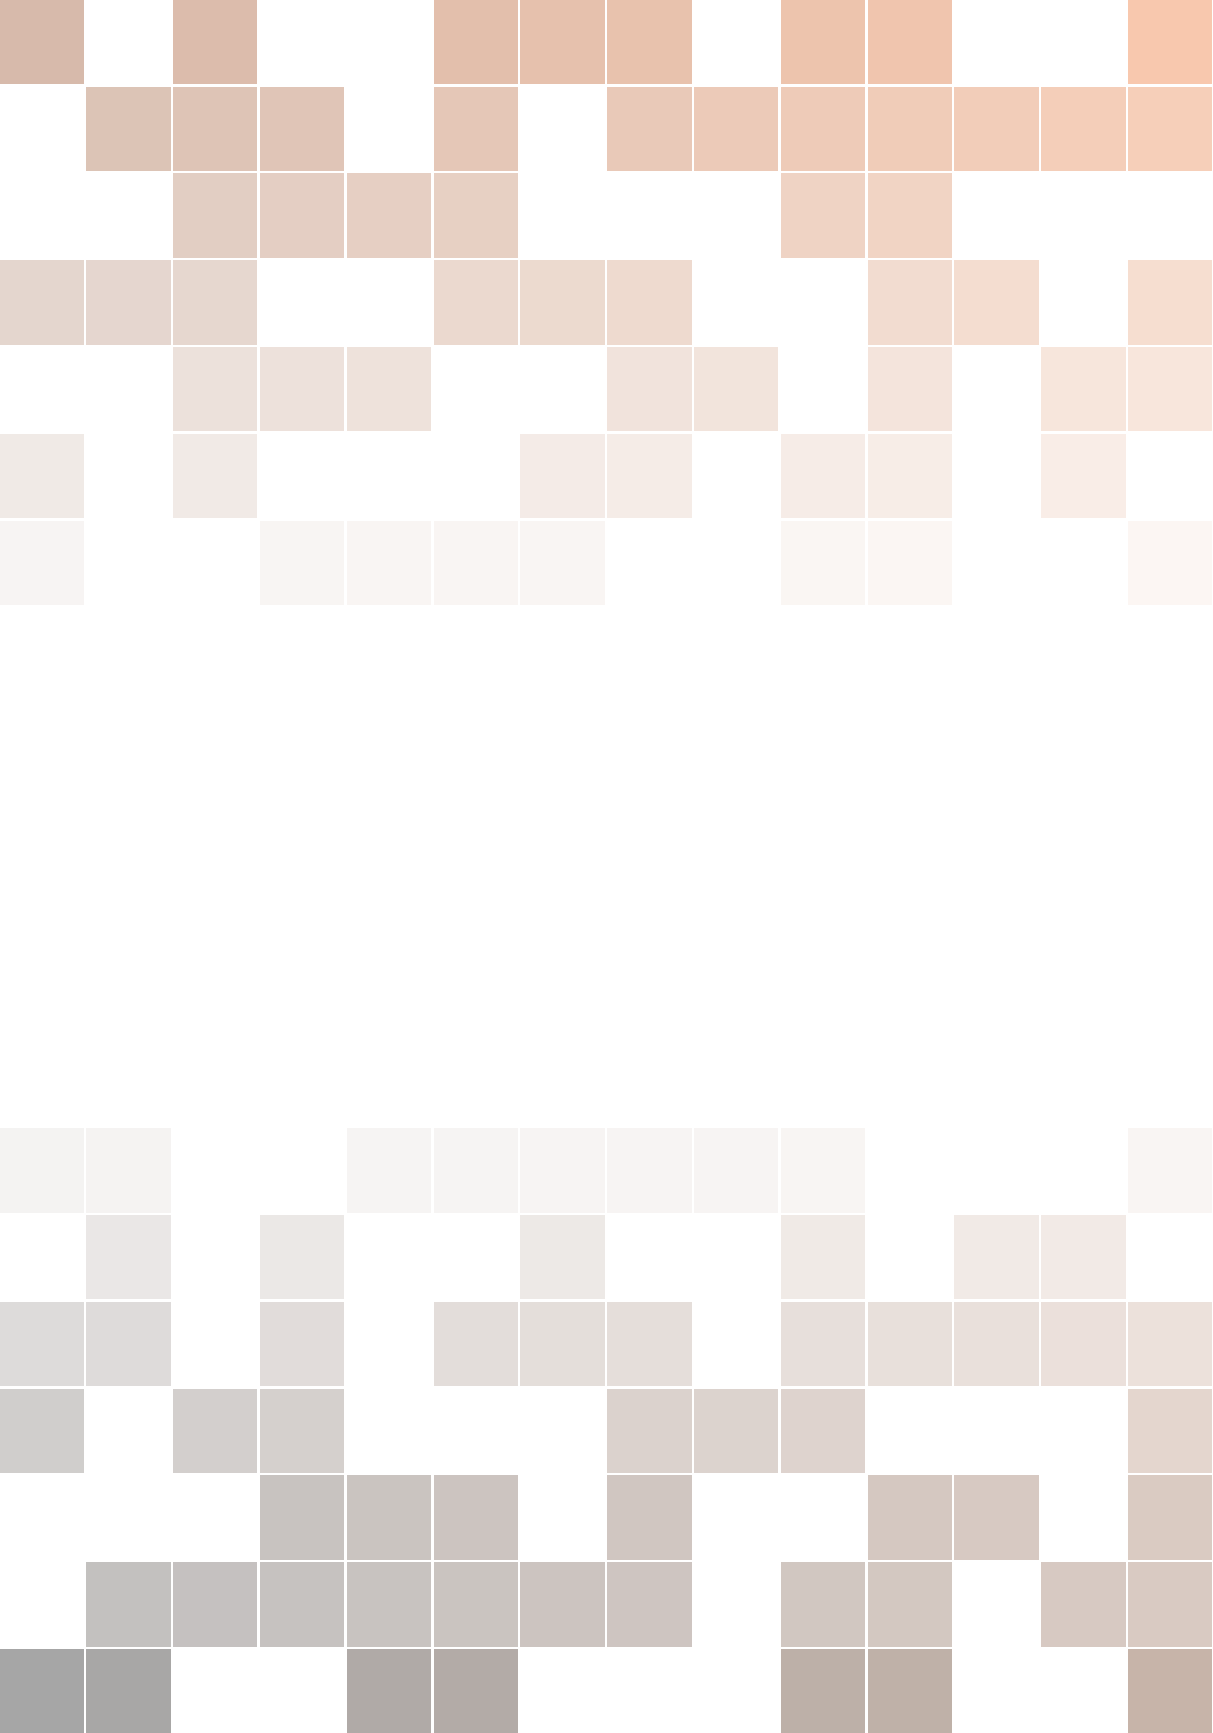
\includegraphics[width=\paperwidth]{background.pdf}};
\draw (current page.center) node [fill=ocre!30!white,fill opacity=0.6,text opacity=1,inner sep=1cm]{\Huge\centering\bfseries\sffamily\parbox[c][][t]{\paperwidth}{\centering Aquele com o glossário de Friends\\[15pt] % Book title
{\Large Entenda as referências da série}\\[20pt] % Subtitle
{\Large Átila \& Sinara}\\[10pt] % Author name
{\Huge CAMURÇA}
}};
\end{tikzpicture}
\vfill
\endgroup

%----------------------------------------------------------------------------------------
%	COPYRIGHT PAGE
%----------------------------------------------------------------------------------------

\newpage
~\vfill
\thispagestyle{empty}

\noindent Copyright \copyright\ 2020 Átila \& Sinara Camurça\\ % Copyright notice

\noindent \textsc{Publicação Independente}\\ % Publisher

\noindent \textsc{https://glossario-friends.netlify.app/}\\ % URL

\noindent Licensed under the Creative Commons Attribution-NonCommercial 3.0 Unported License (the ``License''). You may not use this file except in compliance with the License. You may obtain a copy of the License at \url{http://creativecommons.org/licenses/by-nc/3.0}. Unless required by applicable law or agreed to in writing, software distributed under the License is distributed on an \textsc{``as is'' basis, without warranties or conditions of any kind}, either express or implied. See the License for the specific language governing permissions and limitations under the License.\\ % License information, replace this with your own license (if any)

\noindent \textit{First printing, 2020} % Printing/edition date

%----------------------------------------------------------------------------------------
%	TABLE OF CONTENTS
%----------------------------------------------------------------------------------------

\usechapterimagefalse % If you don't want to include a chapter image, use this to toggle images off - it can be enabled later with \usechapterimagetrue

\chapterimage{chapter_head_1.pdf} % Table of contents heading image

\pagestyle{empty} % Disable headers and footers for the following pages

\tableofcontents % Print the table of contents itself

\cleardoublepage % Forces the first chapter to start on an odd page so it's on the right side of the book

\pagestyle{fancy} % Enable headers and footers again

%\chapterimage{chapter_head_2.pdf} % Chapter heading image

\part{Temporada Um}

\chapter{Aquele onde Tudo começou}

\textbf{RESUMO $\looparrowright$} Rachel foge do casamento e se encontra com os amigos na cafeteria. Ross está deprimido com seu divórcio, mas continua apaixonado por Rachel.

\begin{flushright}
\textcolor{gray600}{Exibido em 21 de Setembro de 1994}
\end{flushright}
\hypertarget{mr.-potato-head}{%
\section{Mr.~Potato Head}\label{mr.-potato-head}}

\begin{figure}[!ht]
  \begin{adjustwidth}{-\oddsidemargin-1in}{-\rightmargin}
    \centering
    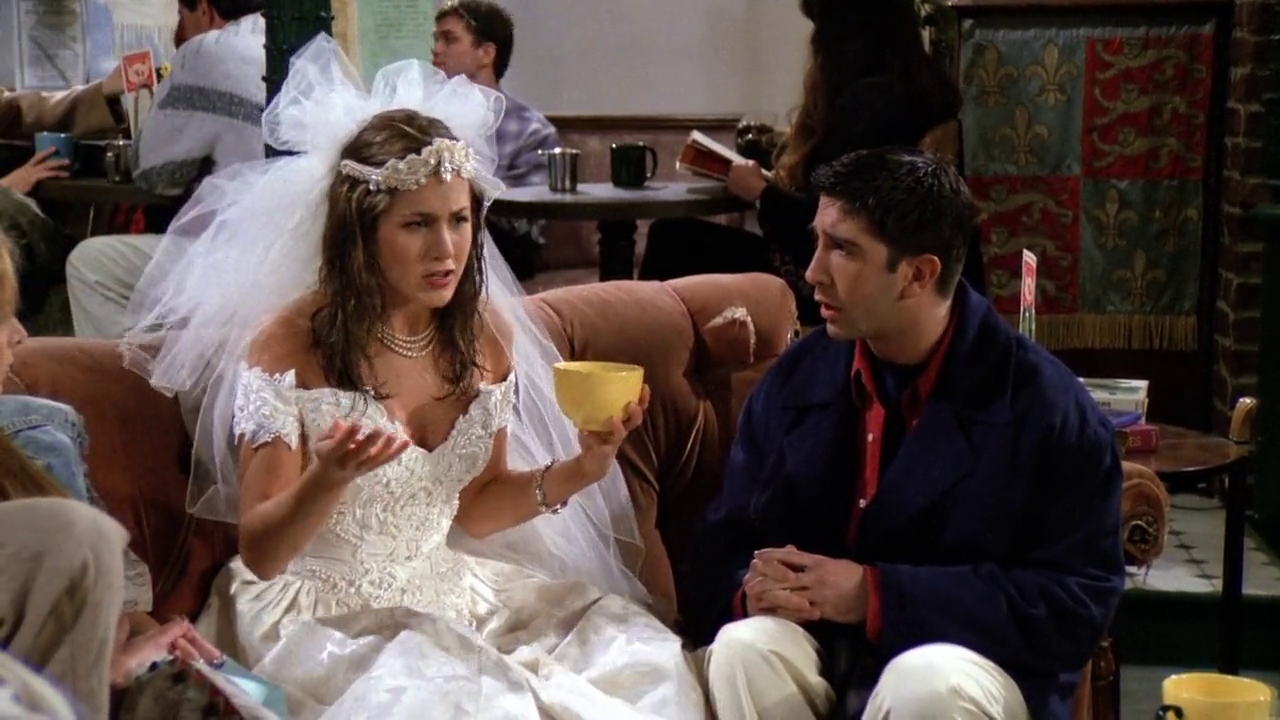
\includegraphics[trim={0 5cm 0 2cm,}, clip, width=\paperwidth]{./S01/img/1/mr-potato-head.png}
    \caption{Mr. Potato Head\label{fig:mr-potato-head}}
  \end{adjustwidth}
\end{figure}

\begin{tcolorbox}[enhanced,center upper,
    drop fuzzy shadow southeast, boxrule=0.3pt,
    lower separated=false,
    colframe=black!30!dialogoBorder,colback=white]
\begin{minipage}[c]{0.14\linewidth}
  \raisebox{\dimexpr-\height+\ht\strutbox\relax}{
    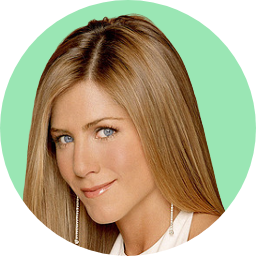
\includegraphics[width=1.5cm]{./assets/img/rachel.png}
  }
   & \centering \scriptsize{Rachel}
\end{minipage}
\hspace{.1mm}
\begin{minipage}[c]{0.8\linewidth}
  \textbf{- [...] and that's when it hit me: How much Barry looks like Mr. Potato Head.}\\
  - [...] e me dei conta: O quanto Barry se parece com o Mr. Potato Head.
\end{minipage}
\end{tcolorbox}

\saveparinfos
\noindent
\begin{minipage}[c]{0.5\textwidth}\useparinfo

Rachel menciona que Barry, seu ex-noivo, parece com o \emph{Mr.~Potato
Head.} Trata-se de um brinquedo inventado por George Lerner, lançado
pela Hasbro em 1952. Em sua versão original havia apenas as partes, tais
como: os olhos, as orelhas e a boca, e era obrigação dos pais fornecerem
uma batata de verdade para formar a cabeça.

O \emph{Mr.~Potato Head} também pode ser visto nos filmes de \emph{Toy
Story} (1995, 1999, 2010, 2019), como um dos brinquedos do Andy.

\end{minipage}\hfill
\begin{minipage}[c]{0.45\textwidth}

\begin{figure}
  \centering
  \begin{tikzpicture}
    \node [inner sep=0pt] at (0,0) {
      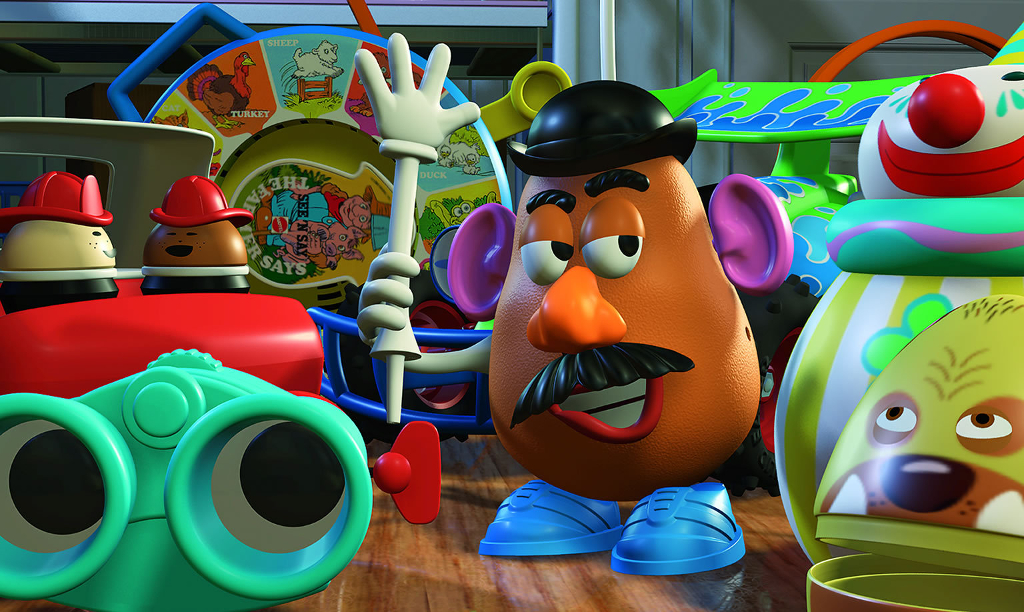
\includegraphics[width=0.8\textwidth,keepaspectratio]{./S01/img/1/mr-potato-head-toy-story.jpg}
    };
    \draw [white, rounded corners=\ClipSep, line width=\ClipSep]
    (current bounding box.north west) --
    (current bounding box.north east) --
    (current bounding box.south east) --
    (current bounding box.south west) -- cycle
    ;
    \end{tikzpicture}
    \caption{Mr. Potato Head (Toy Story)\label{fig:mr-potato-head-toy-story}}
\end{figure}

\end{minipage}

\hypertarget{referuxeancias}{%
\subsection{Referências}\label{referuxeancias}}

\begin{itemize}
\tightlist
\item
  \sloppy V&A Museum of Childhood. \url{https://www.vam.ac.uk/moc/collections/mr-potato-head/}
\item
  \sloppy Toy Story (IMDB). \url{https://www.imdb.com/title/tt0114709/}
\end{itemize}

\hypertarget{tres-destinos}{%
\section{Tres Destinos}\label{tres-destinos}}

\begin{figure}[!ht]
  \begin{adjustwidth}{-\oddsidemargin-1in}{-\rightmargin}
    \centering
    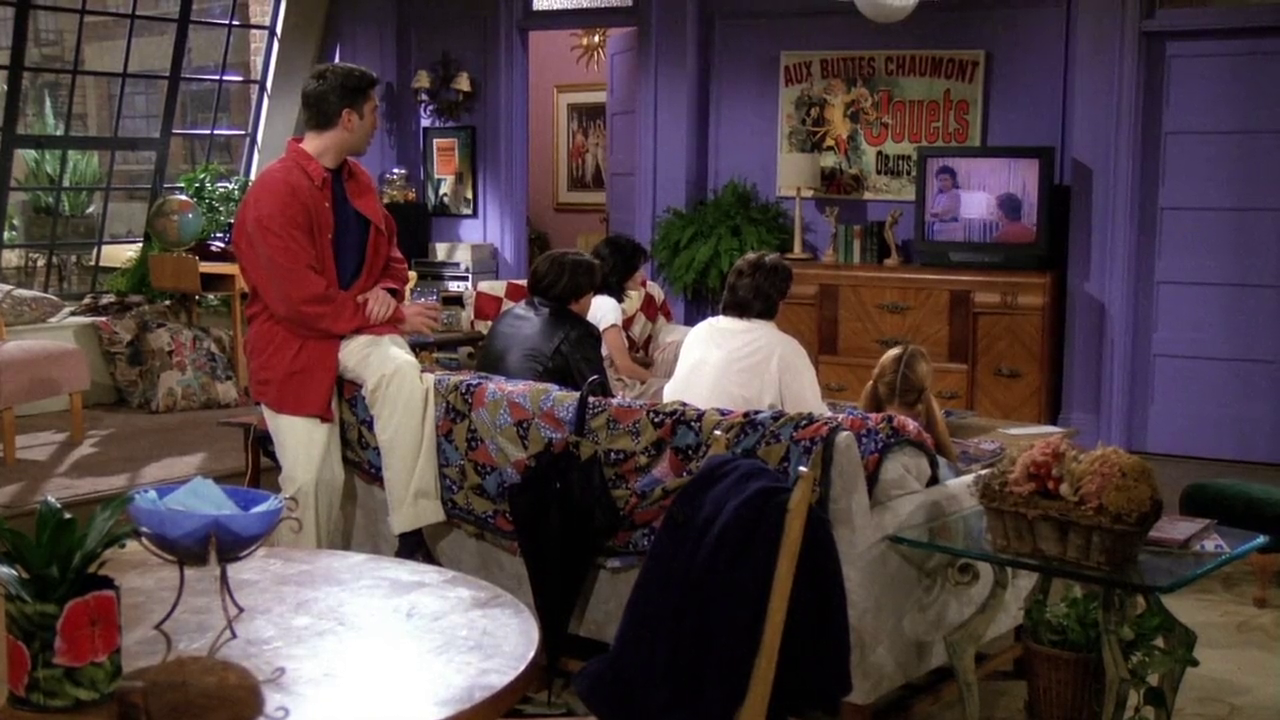
\includegraphics[trim={0 7cm 0 1.5cm,}, clip, width=\paperwidth]{./S01/img/1/tres-destinos.png}
    \caption{Tres Destinos\label{fig:tres-destinos}}
  \end{adjustwidth}
\end{figure}

Os amigos são vistos assistindo a telenovela \emph{Tres Destinos}
(1993), produzida para o mercado hispânico nos Estados Unidos. É a
clássica novela mexicana, do tipo popularmente exibida no Brasil, que
conta a história de 3 jovens irmãs unidas e separadas pelo mesmo homem,
com todos os ingredientes usuais: intriga, paixão, vingança, ódio,
ternura e amor.

\hypertarget{referuxeancias-1}{%
\subsection{Referências}\label{referuxeancias-1}}

\begin{itemize}
\tightlist
\item
  \sloppy EcuRed. \url{https://www.ecured.cu/Tres_destinos_(Telenovela)}
\item
  \sloppy IMDB. \url{https://www.imdb.com/title/tt0211876/}
\item
  \sloppy Abertura (YouTube). \url{https://www.youtube.com/watch?v=kfIk131FZxU}
\end{itemize}

\hypertarget{my-favorite-things}{%
\section{My Favorite Things}\label{my-favorite-things}}

\begin{figure}[!ht]
  \begin{adjustwidth}{-\oddsidemargin-1in}{-\rightmargin}
    \centering
    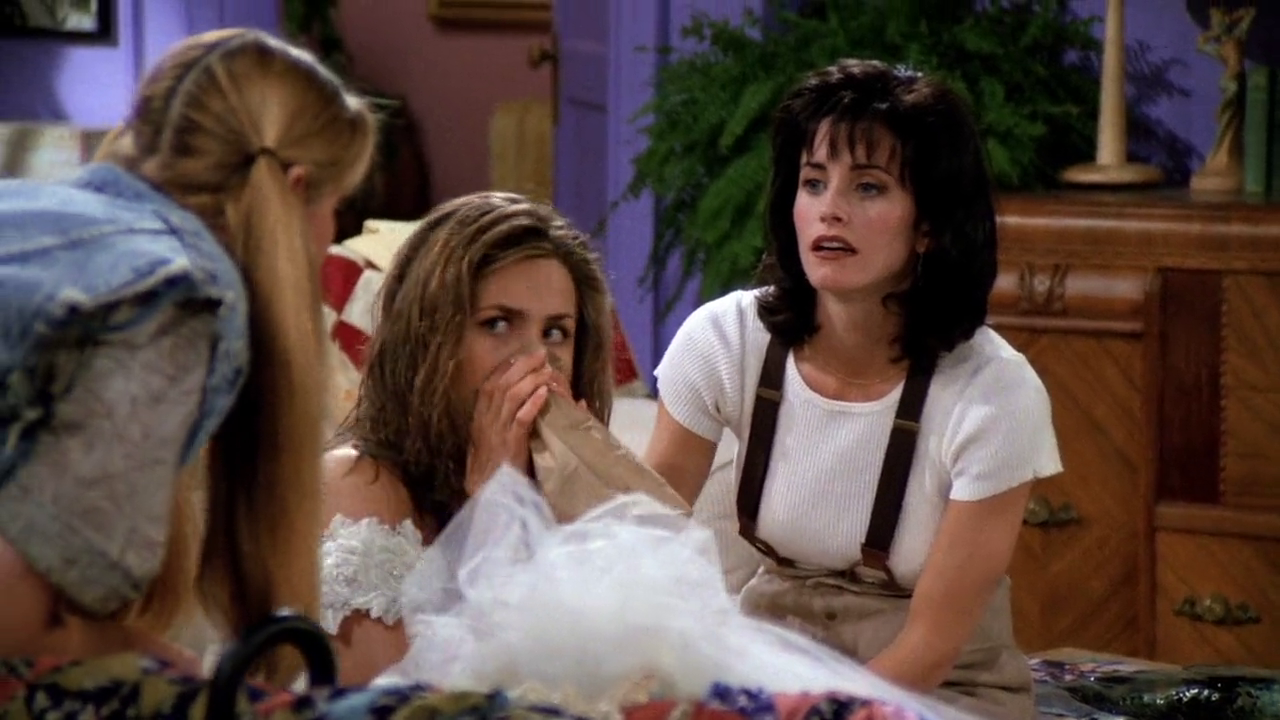
\includegraphics[trim={0 6cm 0 0.5cm,}, clip, width=\paperwidth]{./S01/img/1/my-favorite-things.png}
    \caption{My Favorite Things\label{fig:my-favorite-things}}
  \end{adjustwidth}
\end{figure}

Para acalmar Rachel, Phoebe canta uma versão própria da música \emph{My
Favorite Things} do musical \emph{The Sound of Music} (1959). Em 1965
foi lançado o filme, conhecido no Brasil como \emph{A Noviça Rebelde.}

A música expressa que você deve lembrar de suas coisas favoritas sempre
que se sentir triste.

\bigskip
\begin{tcolorbox}[enhanced,
    drop fuzzy shadow southeast, boxrule=0.3pt,
    lower separated=false, sidebyside, sidebyside align=top,
    halign=flush right, halign lower=left,
    colframe=black!30!dialogoBorder,colback=musicaBg]
\includegraphics[width=0.4cm]{./assets/img/icon-music.png}\\
When I’m feeling sad\\I simply remember my favorite things\\
\tcblower
\includegraphics[width=0.4cm]{./assets/img/icon-language.png}\\
Quando me sinto triste\\Simplesmente lembro de minhas coisas favoritas\\
\end{tcolorbox}

\begin{center}\rule{0.5\linewidth}{0.5pt}\end{center}

Versão da Phoebe:

\bigskip
\begin{tcolorbox}[enhanced,
    drop fuzzy shadow southeast, boxrule=0.3pt,
    lower separated=false, sidebyside, sidebyside align=top,
    halign=flush right, halign lower=left,
    colframe=black!30!dialogoBorder,colback=musicaBg]
\includegraphics[width=0.4cm]{./assets/img/icon-music.png}\\
Raindrops on roses\\And whiskers on kittens\\Doorbells and sleigh bells\\And something with mittens\\La la la la something with strings\\
\tcblower
\includegraphics[width=0.4cm]{./assets/img/icon-language.png}\\
Pingos de chuva em rosas\\E bigodes de gatinhos\\Campainhas e sinos\\E algo com luvas de lã\\La la la la algo com cordas\\
\end{tcolorbox}

Versão original:

\bigskip
\begin{tcolorbox}[enhanced,
    drop fuzzy shadow southeast, boxrule=0.3pt,
    lower separated=false, sidebyside, sidebyside align=top,
    halign=flush right, halign lower=left,
    colframe=black!30!dialogoBorder,colback=musicaBg]
\includegraphics[width=0.4cm]{./assets/img/icon-music.png}\\
Raindrops on roses\\And whiskers on kittens\\Bright copper kettles\\And warm woolen mittens\\Brown paper packages\\Tied up with strings\\
\tcblower
\includegraphics[width=0.4cm]{./assets/img/icon-language.png}\\
Pingos de chuva em rosas\\E bigodes de gatinhos\\Brilhantes tachos de cobre\\E quentes luvas de lã\\Pacotes de papel pardo\\Amarrado com cordas\\
\end{tcolorbox}

\begin{tcolorbox}[enhanced,center upper,
    drop fuzzy shadow southeast, boxrule=0.3pt,
    lower separated=false,
    colframe=black!30!dialogoBorder,colback=white]
\begin{minipage}[c]{0.14\linewidth}
  \raisebox{\dimexpr-\height+\ht\strutbox\relax}{
    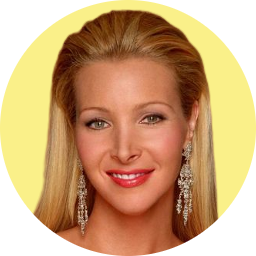
\includegraphics[width=1.5cm]{./assets/img/phoebe.png}
  }
   & \centering \scriptsize{Phoebe}
\end{minipage}
\hspace{.1mm}
\begin{minipage}[c]{0.8\linewidth}
  \textbf{- I helped.}\\
  - Eu ajudei.
\end{minipage}
\end{tcolorbox}

\hypertarget{referuxeancias-2}{%
\subsection{Referências}\label{referuxeancias-2}}

\begin{itemize}
\tightlist
\item
  \sloppy Trecho do filme The Sound of Music, em que é possível ouvir My Favorite Things (Youtube). \url{https://www.youtube.com/watch?v=DGABqdbtQnA}
\item
  \sloppy Wikipédia. \url{https://en.wikipedia.org/wiki/My_Favorite_Things_(song)}
\item
  \sloppy A Noviça Rebelde (IMDB). \url{https://www.imdb.com/title/tt0059742/}
\item
  \sloppy Letra e tradução - Vagalume. \url{https://www.vagalume.com.br/julie-andrews/my-favorite-things-traducao.html}
\end{itemize}

\hypertarget{maina-la-voyante}{%
\section{Maina La Voyante}\label{maina-la-voyante}}

\begin{figure}[!ht]
  \begin{adjustwidth}{-\oddsidemargin-1in}{-\rightmargin}
    \centering
    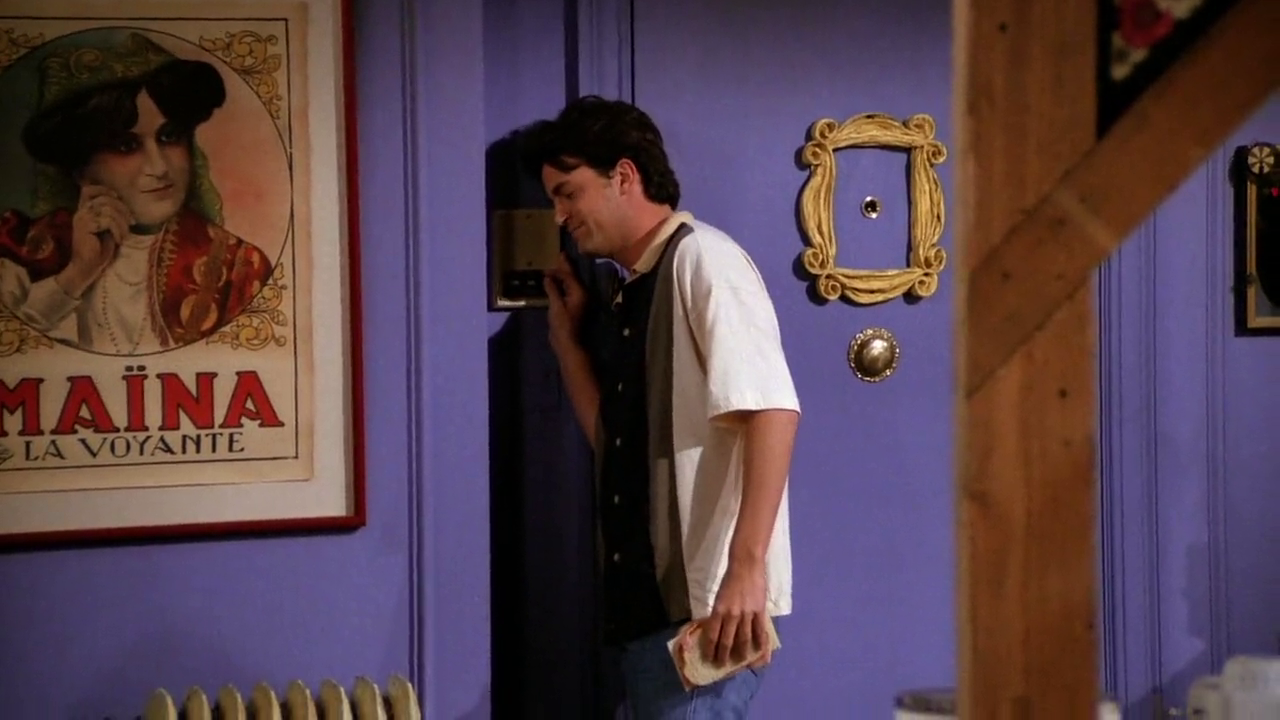
\includegraphics[trim={0 8cm 0 0.5cm,}, clip, width=\paperwidth]{./S01/img/1/maina-la-voyante.png}
    \caption{Maina La Voyante\label{fig:maina-la-voyante}}
  \end{adjustwidth}
\end{figure}

\saveparinfos
\noindent
\begin{minipage}[c]{0.5\textwidth}\useparinfo

Quando Chandler vai atender ao interfone, o poster \emph{Maina La
Voyante} pode ser visto, obra do ilustrador francês Louis Galice
(1864-1935).

\end{minipage}\hfill
\begin{minipage}[c]{0.6\textwidth}

\begin{figure}
  \centering
  \begin{tikzpicture}
    \node [inner sep=0pt] at (0,0) {
      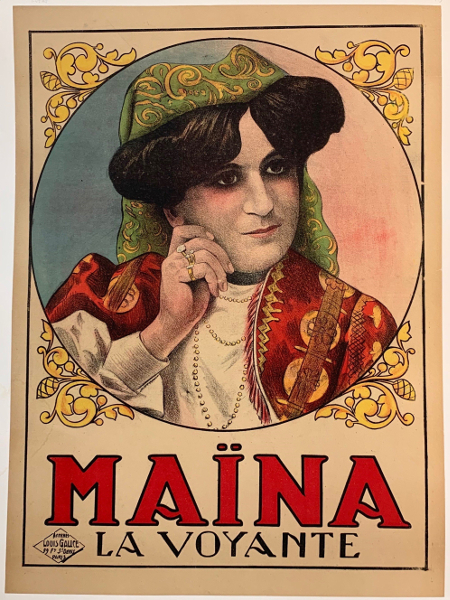
\includegraphics[width=0.6\textwidth,keepaspectratio]{./S01/img/1/maina-la-voyante-poster.jpg}
    };
    \draw [white, rounded corners=\ClipSep, line width=\ClipSep]
    (current bounding box.north west) --
    (current bounding box.north east) --
    (current bounding box.south east) --
    (current bounding box.south west) -- cycle
    ;
    \end{tikzpicture}
    \caption{Maina La Voyante - Poster\label{fig:maina-la-voyante-poster}}
\end{figure}

\end{minipage}

\hypertarget{referuxeancias-3}{%
\subsection{Referências}\label{referuxeancias-3}}

\begin{itemize}
\tightlist
\item
  \sloppy PosterMuseum. \url{https://postermuseum.com/products/maina-la-voyante}
\end{itemize}

\hypertarget{speed-racer}{%
\section{Speed Racer}\label{speed-racer}}

\begin{figure}[!ht]
  \begin{adjustwidth}{-\oddsidemargin-1in}{-\rightmargin}
    \centering
    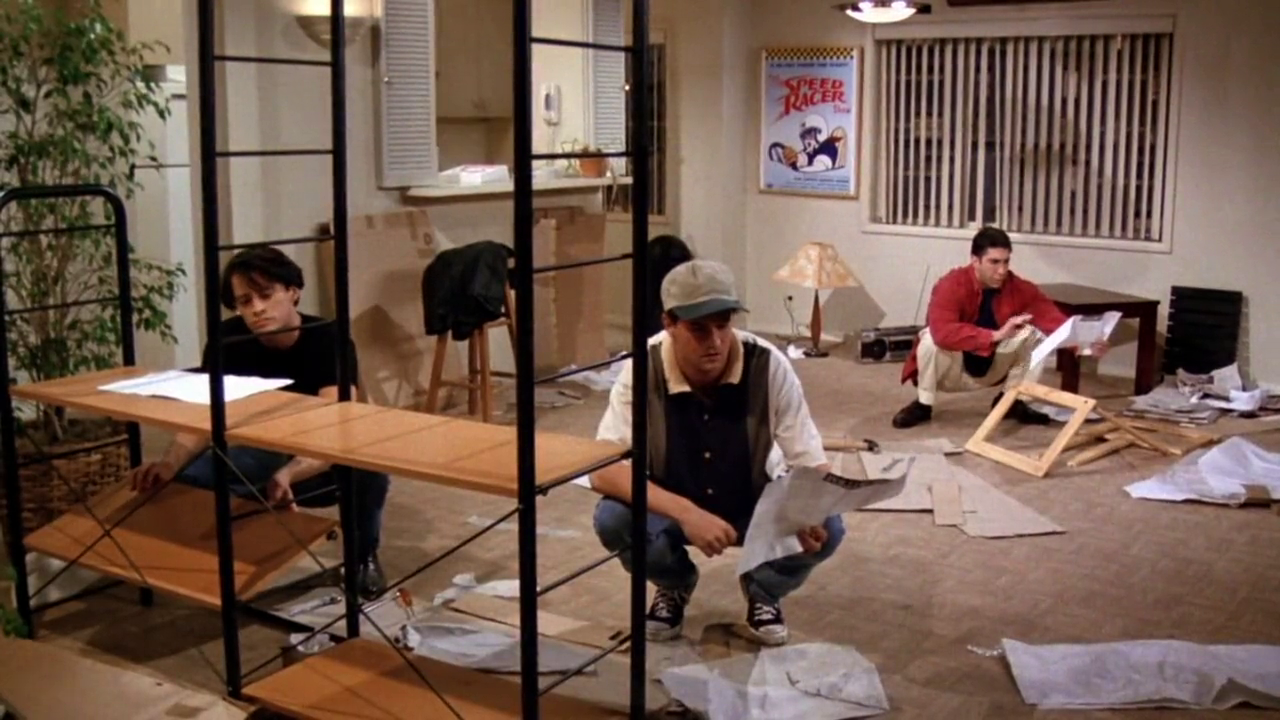
\includegraphics[trim={0 10cm 0 1cm,}, clip, width=\paperwidth]{./S01/img/1/speed-racer.png}
    \caption{Speed Racer\label{fig:speed-racer}}
  \end{adjustwidth}
\end{figure}

\saveparinfos
\noindent
\begin{minipage}[c]{0.5\textwidth}\useparinfo

No novo apartamento do Ross, é possível ver um poster de \emph{The Speed
Racer Show} (1967--1968) produzida pela \emph{Tatsunoko Production}.
Trata-se de uma série japonesa animada protagonizada por \emph{Go
Mifune}, conhecido como \emph{Speed Racer}. É baseada no mangá
\emph{Mach Go Go Go} (1966) criada por \emph{Tatsuo Yoshida}.

\end{minipage}\hfill
\begin{minipage}[c]{0.5\textwidth}

\begin{figure}
  \centering
  \begin{tikzpicture}
    \node [inner sep=0pt] at (0,0) {
      
\includegraphics[width=0.8\textwidth,keepaspectratio]{./S01/img/1/speed-racer-poster.jpeg}
    };
    \draw [white, rounded corners=\ClipSep, line width=\ClipSep]
    (current bounding box.north west) --
    (current bounding box.north east) --
    (current bounding box.south east) --
    (current bounding box.south west) -- cycle
    ;
    \end{tikzpicture}
    \caption{Speed Racer poster\label{fig:speed-racer-poster}}
\end{figure}

\end{minipage}

\hypertarget{referuxeancias-4}{%
\subsection{Referências}\label{referuxeancias-4}}

\begin{itemize}
\tightlist
\item
  \sloppy IMDB. \url{https://www.imdb.com/title/tt0061300/}
\item
  \sloppy Review do Omelete. \url{https://www.omelete.com.br/series-tv/lembra-desse-speed-racer-a-serie-original}
\item
  \sloppy Abertura (YouTube). \url{https://www.youtube.com/watch?v=suCm1w_KTiY}
\end{itemize}

\hypertarget{joanie-loves-chachi}{%
\section{Joanie Loves Chachi}\label{joanie-loves-chachi}}

\begin{figure}[!ht]
  \begin{adjustwidth}{-\oddsidemargin-1in}{-\rightmargin}
    \centering
    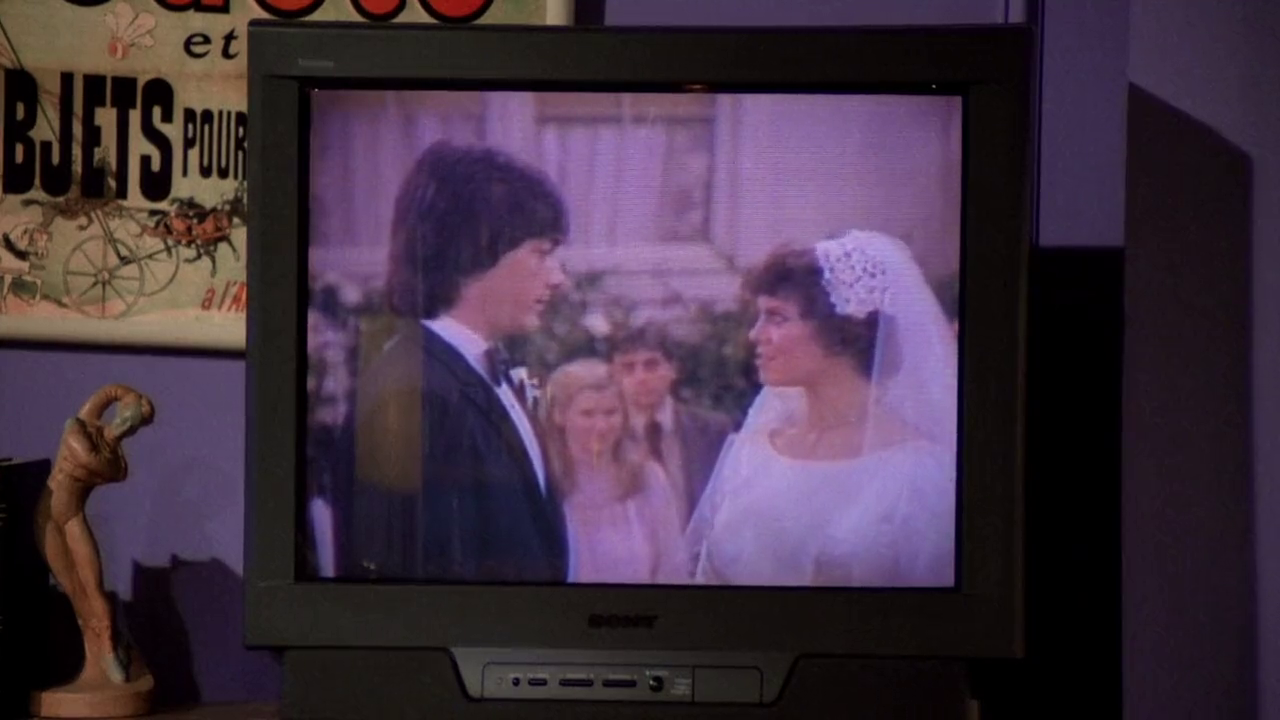
\includegraphics[trim={0 4cm 0 2cm,}, clip, width=\paperwidth]{./S01/img/1/joanie-loves-chachi.png}
    \caption{Joanie Loves Chachi\label{fig:joanie-loves-chachi}}
  \end{adjustwidth}
\end{figure}

\begin{tcolorbox}[enhanced,center upper,
    drop fuzzy shadow southeast, boxrule=0.3pt,
    lower separated=false,
    colframe=black!30!dialogoBorder,colback=white]
\begin{minipage}[c]{0.14\linewidth}
  \raisebox{\dimexpr-\height+\ht\strutbox\relax}{
    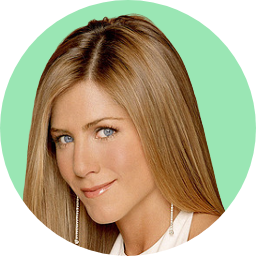
\includegraphics[width=1.5cm]{./assets/img/rachel.png}
  }
   & \centering \scriptsize{Rachel}
\end{minipage}
\hspace{.1mm}
\begin{minipage}[c]{0.8\linewidth}
  \textbf{- But Joanie loved Chachi. That's the difference.}\\
  - Mas Joanie ama Chachi. Essa é a diferença.
\end{minipage}
\end{tcolorbox}

No apartamento de Monica, Rachel, ainda em seu vestido de noiva, assiste
a \emph{Joanie Loves Chachi} (1982--1983) - \emph{spin off} de
\emph{Happy Days} (1974) -, uma série de TV que mostra as aventuras
românticas de Joanie Cunningham e Chachi Arcola, buscando uma carreira
musical em Chicago.

\hypertarget{referuxeancias-5}{%
\subsection{Referências}\label{referuxeancias-5}}

\begin{itemize}
\tightlist
\item
  \sloppy IMDB. \url{https://www.imdb.com/title/tt0083433/}
\item
  \sloppy Wikipédia. \url{https://en.wikipedia.org/wiki/Joanie_Loves_Chachi}
\end{itemize}

\hypertarget{billy-dont-be-a-hero}{%
\section{Billy, don't be a hero}\label{billy-dont-be-a-hero}}

\begin{figure}[!ht]
  \begin{adjustwidth}{-\oddsidemargin-1in}{-\rightmargin}
    \centering
    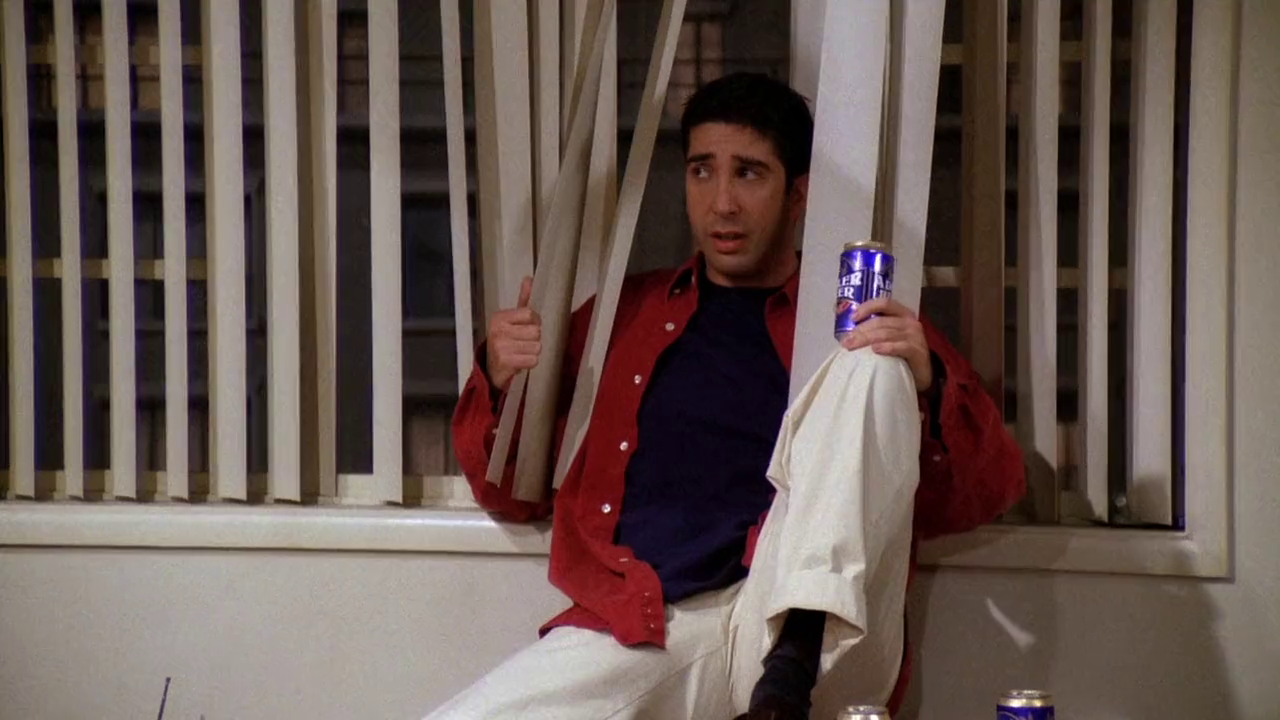
\includegraphics[trim={0 6.5cm 0 2.5cm,}, clip, width=\paperwidth]{./S01/img/1/billy-dont-be-a-hero.png}
    \caption{Billy, don’t be a hero\label{fig:billy-don-t-be-a-hero}}
  \end{adjustwidth}
\end{figure}

\begin{tcolorbox}[enhanced,center upper,
    drop fuzzy shadow southeast, boxrule=0.3pt,
    lower separated=false,
    colframe=black!30!dialogoBorder,colback=white]
\begin{minipage}[c]{0.14\linewidth}
  \raisebox{\dimexpr-\height+\ht\strutbox\relax}{
    
\includegraphics[width=1.5cm]{./assets/img/ross.png}
  }
   & \centering \scriptsize{Ross}
\end{minipage}
\hspace{.1mm}
\begin{minipage}[c]{0.8\linewidth}
  \textbf{- Do the words, 'Billy, don't be a hero', mean anything to you?}\\
  - As palavras, 'Billy, don't be a hero', significam alguma coisa pra vocês?
\end{minipage}
\end{tcolorbox}

\saveparinfos
\noindent
\begin{minipage}[c]{0.5\textwidth}\useparinfo

Ross faz menção a música \emph{Billy, don't be a hero} (1974) composta
por Mitch Murray e Peter Callander. Lançada inicialmente no Reino Unido
na voz de \emph{Paper Lace}, foi logo em seguida lançada também nos
Estados Unidos pelo grupo \emph{Bo Donaldson and The Heywoods.}

\end{minipage}\hfill
\begin{minipage}[c]{0.5\textwidth}

\begin{figure}
  \centering
  \begin{tikzpicture}
    \node [inner sep=0pt] at (0,0) {
      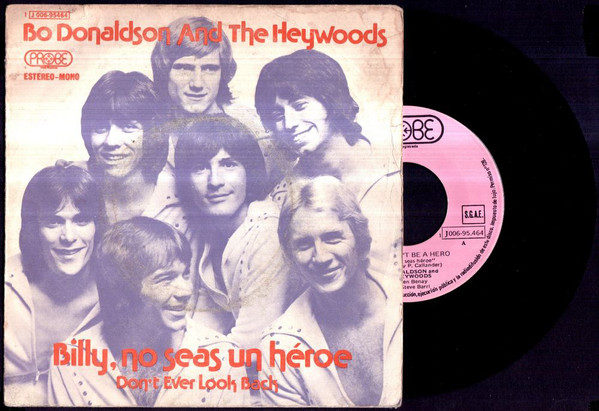
\includegraphics[width=0.8\textwidth,keepaspectratio]{./S01/img/1/billy-dont-be-a-hero-single.jpg}
    };
    \draw [white, rounded corners=\ClipSep, line width=\ClipSep]
    (current bounding box.north west) --
    (current bounding box.north east) --
    (current bounding box.south east) --
    (current bounding box.south west) -- cycle
    ;
    \end{tikzpicture}
    \caption{Billy, don’t be a hero - Single\label{fig:billy-don-t-be-a-hero-single}}
\end{figure}

\end{minipage}

\hypertarget{referuxeancias-6}{%
\subsection{Referências}\label{referuxeancias-6}}

\begin{itemize}
\tightlist
\item
  \sloppy Site Oficial. \url{http://www.bodonaldson.net/}
\item
  \sloppy IMDB. \url{https://en.wikipedia.org/wiki/Billy_Don%27t_Be_a_Hero}
\item
  \sloppy Letra - MetroLyrics. \url{https://www.metrolyrics.com/billy-dont-be-a-hero-lyrics-paper-lace.html}
\item
  \sloppy Billy, don’t be a hero - YouTube. \url{https://www.youtube.com/watch?v=1qlK9TJvuSk}
\end{itemize}

\hypertarget{pinocchio}{%
\section{Pinocchio}\label{pinocchio}}

\begin{figure}[!ht]
  \begin{adjustwidth}{-\oddsidemargin-1in}{-\rightmargin}
    \centering
    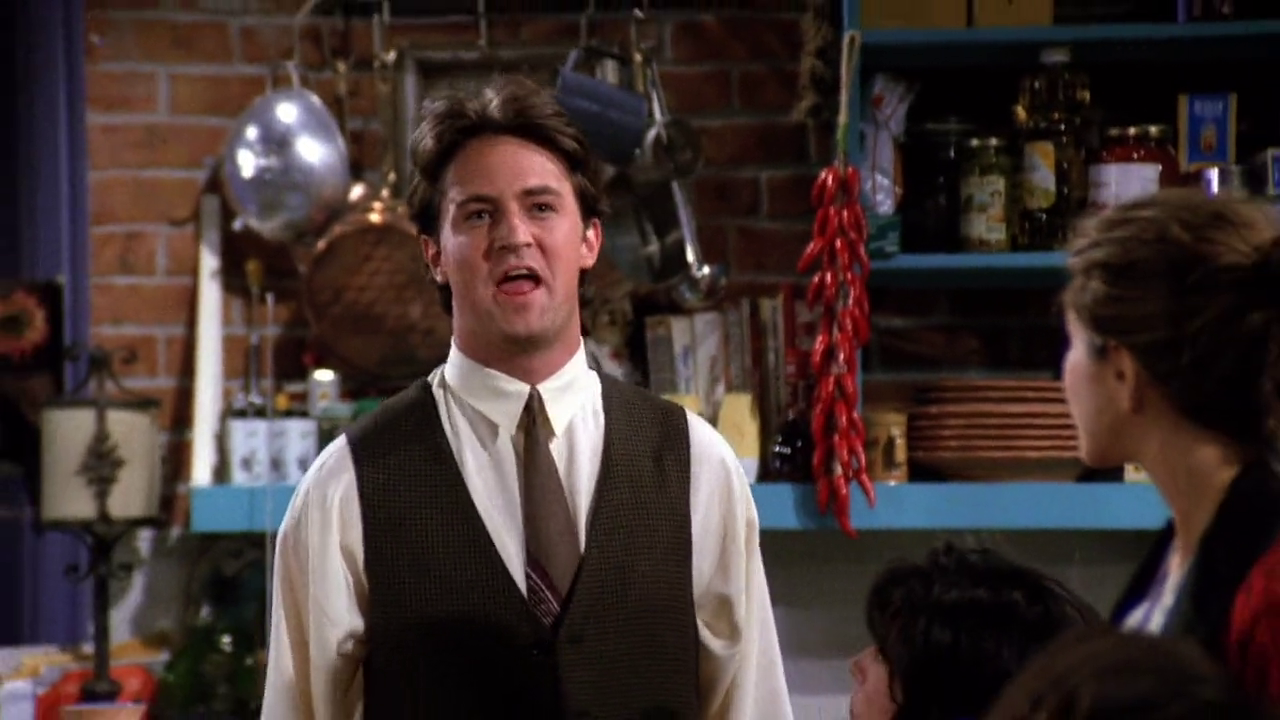
\includegraphics[trim={0 5cm 0 2cm,}, clip, width=\paperwidth]{./S01/img/1/pinocchio.png}
    \caption{Pinocchio\label{fig:pinocchio}}
  \end{adjustwidth}
\end{figure}

\begin{tcolorbox}[enhanced,center upper,
    drop fuzzy shadow southeast, boxrule=0.3pt,
    lower separated=false,
    colframe=black!30!dialogoBorder,colback=white]
\begin{minipage}[c]{0.14\linewidth}
  \raisebox{\dimexpr-\height+\ht\strutbox\relax}{
    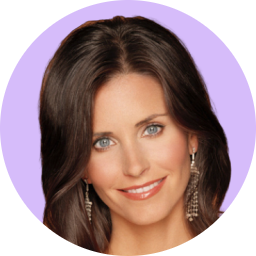
\includegraphics[width=1.5cm]{./assets/img/monica.png}
  }
   & \centering \scriptsize{Monica}
\end{minipage}
\hspace{.1mm}
\begin{minipage}[c]{0.8\linewidth}
  \textbf{- Wait, unless you happened to catch the Reruns' production of Pinocchio.}\\
  - Espera, a não ser que tenha visto a refilmagem do Pinóquio.
\end{minipage}

\medskip
\begin{minipage}[c]{0.14\linewidth}
  \raisebox{\dimexpr-\height+\ht\strutbox\relax}{
    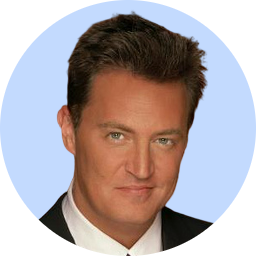
\includegraphics[width=1.5cm]{./assets/img/chandler.png}
  }
   & \centering \scriptsize{Chandler}
\end{minipage}
\hspace{.1mm}
\begin{minipage}[c]{0.8\linewidth}
  \textbf{- Look, Gepetto, I'm a real live boy.}\\
  - Olha, Gepetto, sou um menino de verdade.
\end{minipage}
\end{tcolorbox}

\saveparinfos
\noindent
\begin{minipage}[c]{0.5\textwidth}\useparinfo

Referência ao filme \emph{Pinocchio} (1940) ou \emph{Pinóquio} como
ficou conhecido no Brasil. Produzido pela \emph{Walt Disney}, o filme
conta a história de um velho carpinteiro chamado \emph{Gepetto}, que faz
um boneco de madeira chamado \emph{Pinóquio}, o qual é trazido a vida
pela \emph{Fada Azul}, com a condição de que ele demonstre obediência,
bravura e lealdade a seu criador.

\end{minipage}\hfill
\begin{minipage}[c]{0.5\textwidth}

\begin{figure}
  \centering
  \begin{tikzpicture}
    \node [inner sep=0pt] at (0,0) {
      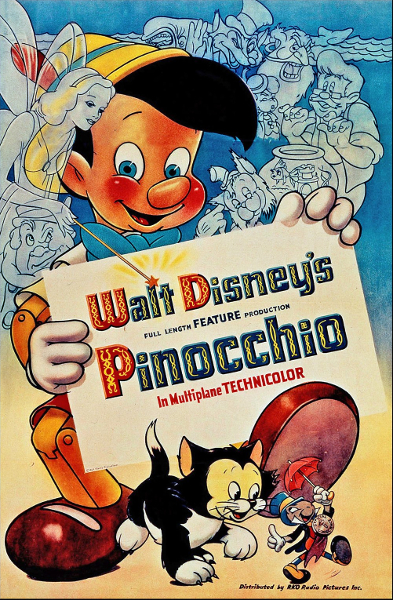
\includegraphics[width=0.5\textwidth,keepaspectratio]{./S01/img/1/pinocchio-poster.jpg}
    };
    \draw [white, rounded corners=\ClipSep, line width=\ClipSep]
    (current bounding box.north west) --
    (current bounding box.north east) --
    (current bounding box.south east) --
    (current bounding box.south west) -- cycle
    ;
    \end{tikzpicture}
    \caption{Pinocchio - Poster\label{fig:pinocchio-poster}}
\end{figure}

\end{minipage}

O filme tem muitos trechos musicais, e é daí que o Chandler retira
inspiração para a música que ele canta ao sair do apartamento:

\bigskip
\begin{tcolorbox}[enhanced,
    drop fuzzy shadow southeast, boxrule=0.3pt,
    lower separated=false, sidebyside, sidebyside align=top,
    halign=flush right, halign lower=left,
    colframe=black!30!dialogoBorder,colback=musicaBg]
\includegraphics[width=0.4cm]{./assets/img/icon-music.png}\\
Once I was a wooden boy,\\a little wooden boy…\\
\tcblower
\includegraphics[width=0.4cm]{./assets/img/icon-language.png}\\
Uma vez eu era um garoto de madeira,\\Um pequeno garoto de madeira…\\
\end{tcolorbox}

\hypertarget{referuxeancias-7}{%
\subsection{Referências}\label{referuxeancias-7}}

\begin{itemize}
\tightlist
\item
  \sloppy IMDB. \url{https://www.imdb.com/title/tt0032910/}
\item
  \sloppy Wikipédia. \url{https://pt.wikipedia.org/wiki/Pin%C3%B3quio_(filme)}
\end{itemize}

\hypertarget{liza-minnelli}{%
\section{Liza Minnelli}\label{liza-minnelli}}

\begin{figure}[!ht]
  \begin{adjustwidth}{-\oddsidemargin-1in}{-\rightmargin}
    \centering
    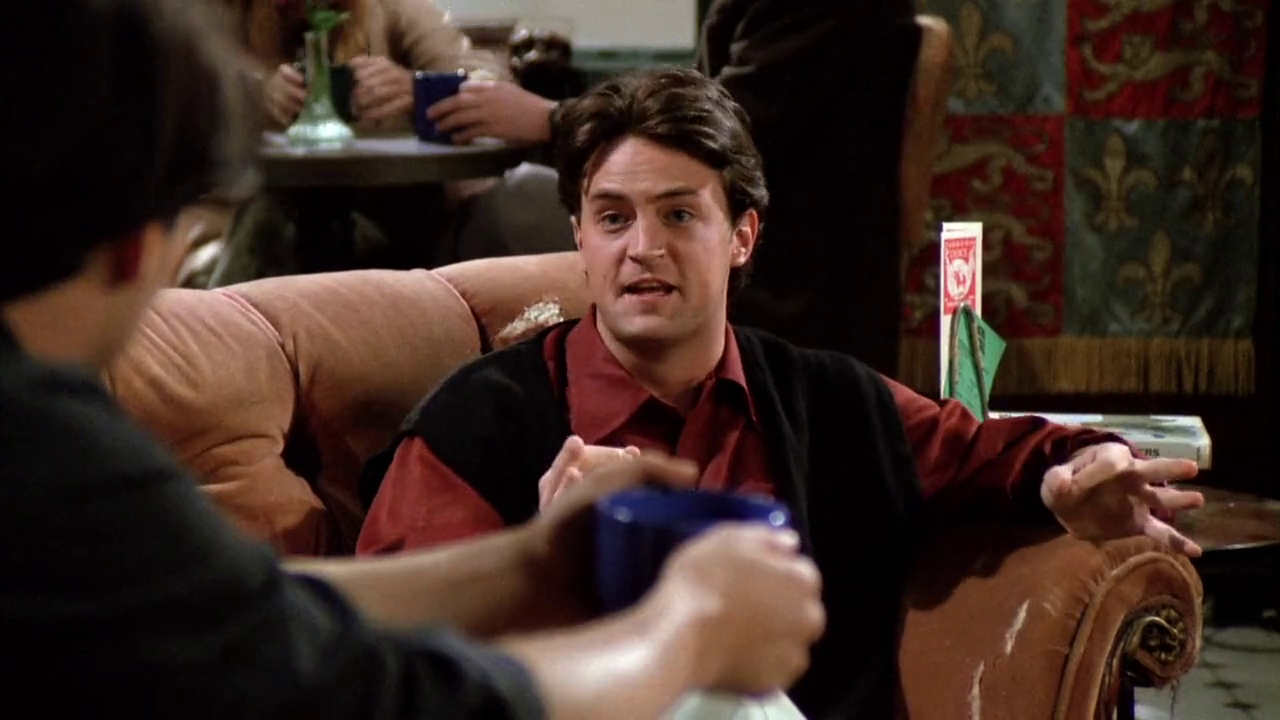
\includegraphics[trim={0 5cm 0 2cm,}, clip, width=\paperwidth]{./S01/img/1/liza-minnelli.png}
    \caption{Liza Minnelli\label{fig:liza-minnelli}}
  \end{adjustwidth}
\end{figure}

\begin{tcolorbox}[enhanced,center upper,
    drop fuzzy shadow southeast, boxrule=0.3pt,
    lower separated=false,
    colframe=black!30!dialogoBorder,colback=white]
\begin{minipage}[c]{0.14\linewidth}
  \raisebox{\dimexpr-\height+\ht\strutbox\relax}{
    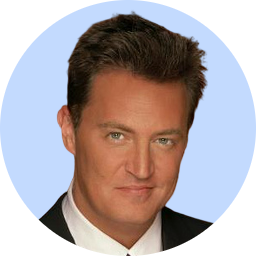
\includegraphics[width=1.5cm]{./assets/img/chandler.png}
  }
   & \centering \scriptsize{Chandler}
\end{minipage}
\hspace{.1mm}
\begin{minipage}[c]{0.8\linewidth}
  \textbf{- Kids, new dream. I'm in Las Vegas. I'm Liza Minnelli.}\\
  - Crianças, novo sonho. Tô em Las Vegas. Eu sou Liza Minelli.
\end{minipage}
\end{tcolorbox}

\saveparinfos
\noindent
\begin{minipage}[c]{0.5\textwidth}\useparinfo

Chandler menciona a atriz e cantora americana \emph{Liza Minnelli}
(1946-), é conhecida por ganhar o Oscar de melhor atriz por sua atuação
no filme \emph{Cabaret} (1972).

\end{minipage}\hfill
\begin{minipage}[c]{0.5\textwidth}

\begin{figure}
  \centering
  \begin{tikzpicture}
    \node [inner sep=0pt] at (0,0) {
      
\includegraphics[width=0.8\textwidth,keepaspectratio]{./S01/img/1/liza-minnelli-cabaret.jpg}
    };
    \draw [white, rounded corners=\ClipSep, line width=\ClipSep]
    (current bounding box.north west) --
    (current bounding box.north east) --
    (current bounding box.south east) --
    (current bounding box.south west) -- cycle
    ;
    \end{tikzpicture}
    \caption{Liza Minnelli - Cabaret\label{fig:liza-minnelli-cabaret}}
\end{figure}

\end{minipage}

\hypertarget{referuxeancias-8}{%
\subsection{Referências}\label{referuxeancias-8}}

\begin{itemize}
\tightlist
\item
  \sloppy IDMB. \url{https://www.imdb.com/name/nm0591485/}
\item
  \sloppy Wikipédia. \url{https://pt.wikipedia.org/wiki/Liza_Minnelli}
\end{itemize}


\chapter{Aquele com o Ultrassom no Final}

\textbf{RESUMO $\looparrowright$} A ex-mulher de Ross está grávida dele, mas ele não gosta do sobrenome que ela escolheu para o bebê.

\begin{flushright}
\textcolor{gray600}{Exibido em 28 de Setembro de 1994}
\end{flushright}
\hypertarget{pink-floyd}{%
\section{Pink Floyd}\label{pink-floyd}}

\begin{figure}[!ht]
  \begin{adjustwidth}{-\oddsidemargin-1in}{-\rightmargin}
    \centering
    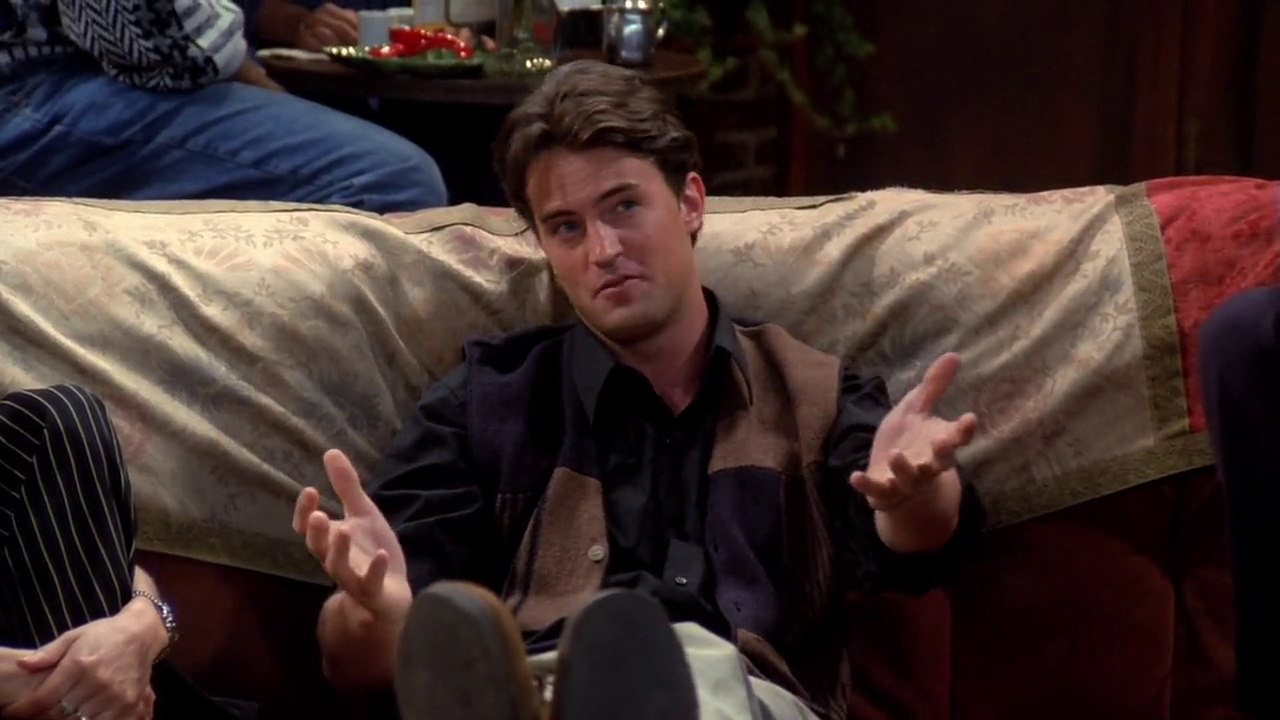
\includegraphics[trim={0 5cm 0 2cm,}, clip, width=\paperwidth]{./S01/img/2/pink-floyd.png}
    \caption{Pink Floyd\label{fig:pink-floyd}}
  \end{adjustwidth}
\end{figure}

\begin{tcolorbox}[enhanced,center upper,
    drop fuzzy shadow southeast, boxrule=0.3pt,
    lower separated=false,
    colframe=black!30!dialogoBorder,colback=white]
\begin{minipage}[c]{0.14\linewidth}
  \raisebox{\dimexpr-\height+\ht\strutbox\relax}{
    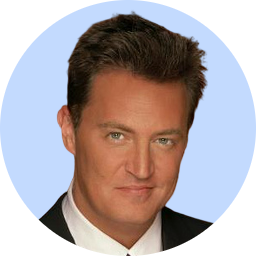
\includegraphics[width=1.5cm]{./assets/img/chandler.png}
  }
   & \centering \scriptsize{Chandler}
\end{minipage}
\hspace{.1mm}
\begin{minipage}[c]{0.8\linewidth}
  \textbf{- ...before Pink Floyd comes out.}\\
  - ...antes do show do Pink Floyd.
\end{minipage}
\end{tcolorbox}

Chandler menciona a banda britânica de rock progressivo \emph{Pink
Floyd}, formada em 1965. A banda lança o albúm \emph{The Division Bell}
em Março 1994, um pouco antes do começo da série.

\begin{figure}
  \centering
  \begin{tikzpicture}
    \node [inner sep=0pt] at (0,0) {
      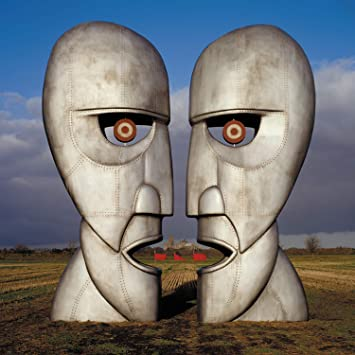
\includegraphics[width=0.5\textwidth,keepaspectratio]{./S01/img/2/the-division-bell.jpg}
    };
    \draw [white, rounded corners=\ClipSep, line width=\ClipSep]
    (current bounding box.north west) --
    (current bounding box.north east) --
    (current bounding box.south east) --
    (current bounding box.south west) -- cycle
    ;
    \end{tikzpicture}
    \caption{The Division Bell\label{fig:the-division-bell}}
\end{figure}

\hypertarget{referuxeancias}{%
\subsection{Referências}\label{referuxeancias}}

\begin{itemize}
\tightlist
\item
  \sloppy Site oficial. \url{https://www.pinkfloyd.com/}
\end{itemize}

\hypertarget{threes-company}{%
\section{Three's Company}\label{threes-company}}

\begin{figure}[!ht]
  \begin{adjustwidth}{-\oddsidemargin-1in}{-\rightmargin}
    \centering
    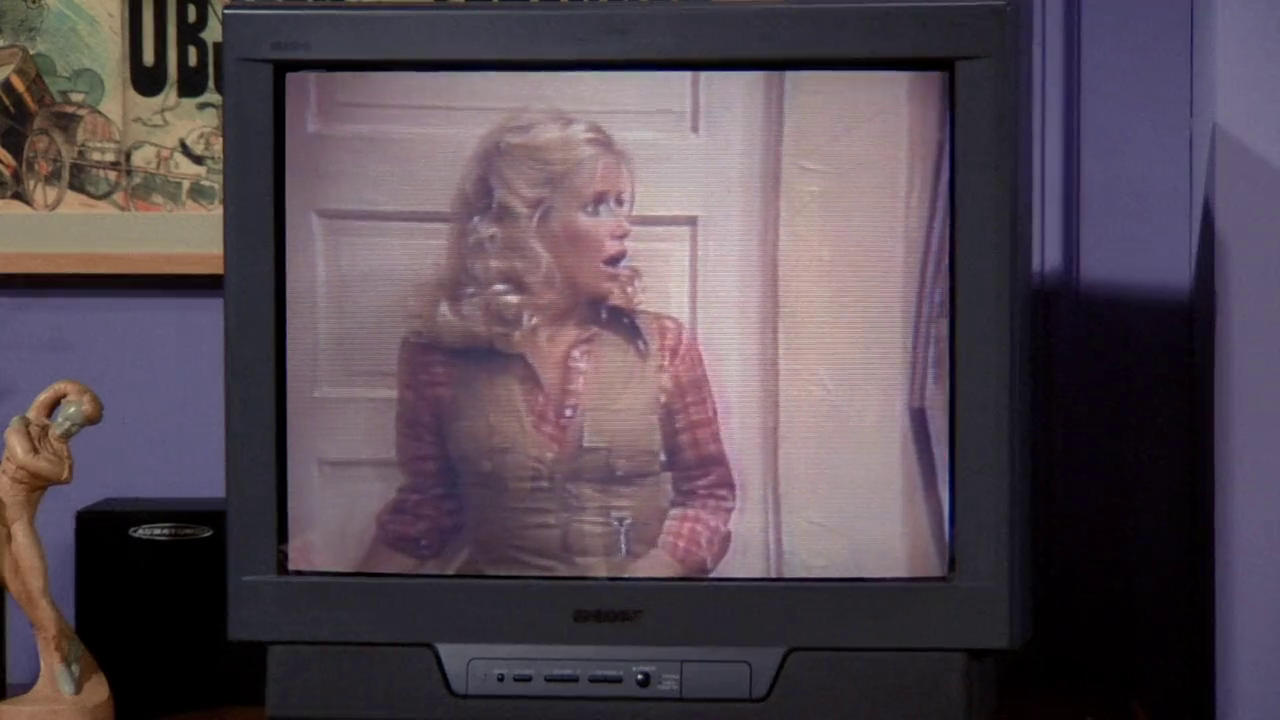
\includegraphics[trim={0 5cm 0 2cm,}, clip, width=\paperwidth]{./S01/img/2/threes-company.png}
    \caption{Three’s Company\label{fig:three-s-company}}
  \end{adjustwidth}
\end{figure}

\begin{tcolorbox}[enhanced,center upper,
    drop fuzzy shadow southeast, boxrule=0.3pt,
    lower separated=false,
    colframe=black!30!dialogoBorder,colback=white]
\begin{minipage}[c]{0.14\linewidth}
  \raisebox{\dimexpr-\height+\ht\strutbox\relax}{
    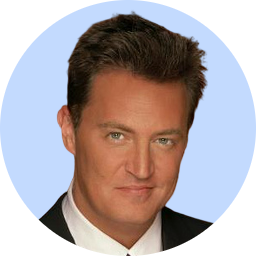
\includegraphics[width=1.5cm]{./assets/img/chandler.png}
  }
   & \centering \scriptsize{Chandler}
\end{minipage}
\hspace{.1mm}
\begin{minipage}[c]{0.8\linewidth}
  \textbf{- I think this is the episode of Three's Company where's there's some kind of misunderstanding.}\\
  - Acho que este é o episódio de Three's Company onde há um mal-entendido.
\end{minipage}

\medskip
\begin{minipage}[c]{0.14\linewidth}
  \raisebox{\dimexpr-\height+\ht\strutbox\relax}{
    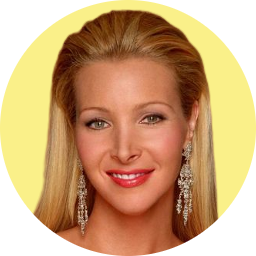
\includegraphics[width=1.5cm]{./assets/img/phoebe.png}
  }
   & \centering \scriptsize{Phoebe}
\end{minipage}
\hspace{.1mm}
\begin{minipage}[c]{0.8\linewidth}
  \textbf{- Then I've already seen this one.}\\
  - Então, eu já vi.
\end{minipage}
\end{tcolorbox}

Chandler, Joey, Phoebe e Monica assistem a \emph{sitcom} \emph{Three's
Company} (1977-1984), conhecida no Brasil como \emph{Um é Pouco, Dois é
Bom e Três é Demais}. Conta a história de Janet e Chrissy que dividem um
apartamento em Santa Monica e conhecem um novo colega Jack. Ele estuda
gastronomia e, quando pedem para ele provar suas capacidades, finge ser
gay. Eles passam a morar juntos e passar por desentendimentos, aventuras
e brincadeiras. Daí a piada, o \emph{plot} da história quase sempre
envolve um desentendimento.

\begin{figure}
  \centering
  \begin{tikzpicture}
    \node [inner sep=0pt] at (0,0) {
      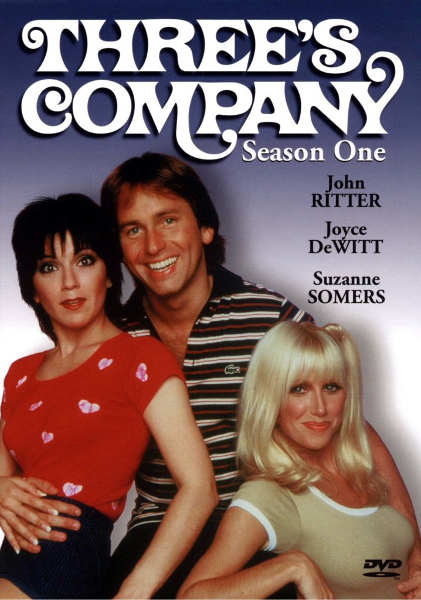
\includegraphics[width=0.4\textwidth,keepaspectratio]{./S01/img/2/threes-company-cover.jpg}
    };
    \draw [white, rounded corners=\ClipSep, line width=\ClipSep]
    (current bounding box.north west) --
    (current bounding box.north east) --
    (current bounding box.south east) --
    (current bounding box.south west) -- cycle
    ;
    \end{tikzpicture}
    \caption{Three’s Company - Cover\label{fig:three-s-company-cover}}
\end{figure}

\hypertarget{referuxeancias-1}{%
\subsection{Referências}\label{referuxeancias-1}}

\begin{itemize}
\tightlist
\item
  \sloppy Site oficial. \url{http://www.threescompany.com/}
\item
  \sloppy Fandom Wiki. \url{https://threescompany.fandom.com/wiki/Three%27s_Company}
\item
  \sloppy Página do Adoro Cinema. \url{http://www.adorocinema.com/series/serie-387/foto-detalhada/?cmediafile=21161912}
\end{itemize}

\hypertarget{thighmaster}{%
\section{Thighmaster}\label{thighmaster}}

\begin{figure}[!ht]
  \begin{adjustwidth}{-\oddsidemargin-1in}{-\rightmargin}
    \centering
    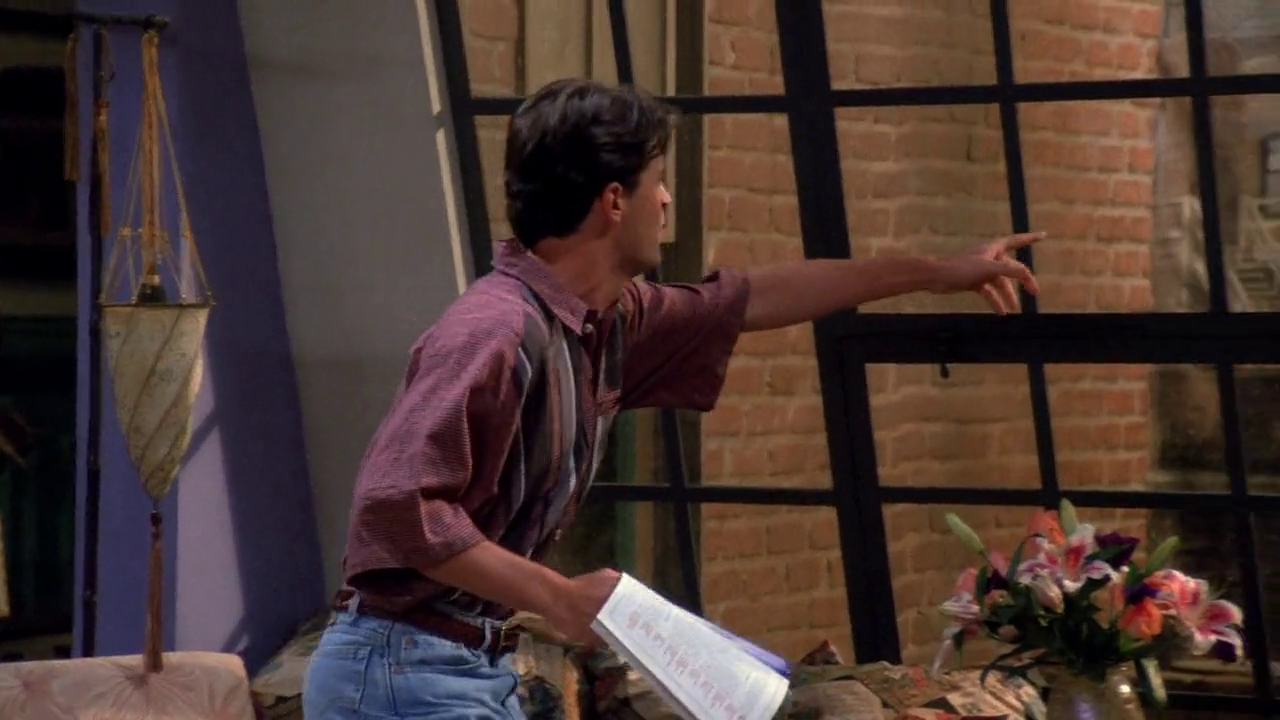
\includegraphics[trim={0 7cm 0 2cm,}, clip, width=\paperwidth]{./S01/img/2/thighmaster.png}
    \caption{Thighmaster\label{fig:thighmaster}}
  \end{adjustwidth}
\end{figure}

\begin{tcolorbox}[enhanced,center upper,
    drop fuzzy shadow southeast, boxrule=0.3pt,
    lower separated=false,
    colframe=black!30!dialogoBorder,colback=white]
\begin{minipage}[c]{0.14\linewidth}
  \raisebox{\dimexpr-\height+\ht\strutbox\relax}{
    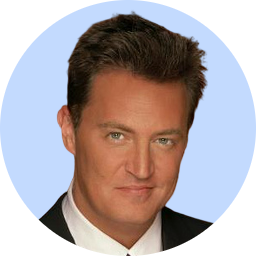
\includegraphics[width=1.5cm]{./assets/img/chandler.png}
  }
   & \centering \scriptsize{Chandler}
\end{minipage}
\hspace{.1mm}
\begin{minipage}[c]{0.8\linewidth}
  \textbf{- Ugly Naked Guy got a Thighmaster.}\\
  - Peladão feio fazendo exercício!
\end{minipage}
\end{tcolorbox}

Chandler menciona que o \emph{Ugly Naked Guy} está usando um
\emph{Thighmaster}, conhecido aparelho aeróbico usado para tonificar a
parte interna da coxa. O interessante aqui é que o \emph{Thighmaster}
está diretamente relacionado à seção \emph{Three's Company}, já que
Suzanne Somers - que faz o papel de Chrissy na série - é a porta voz
oficial do produto.

\begin{figure}
  \centering
  \begin{tikzpicture}
    \node [inner sep=0pt] at (0,0) {
      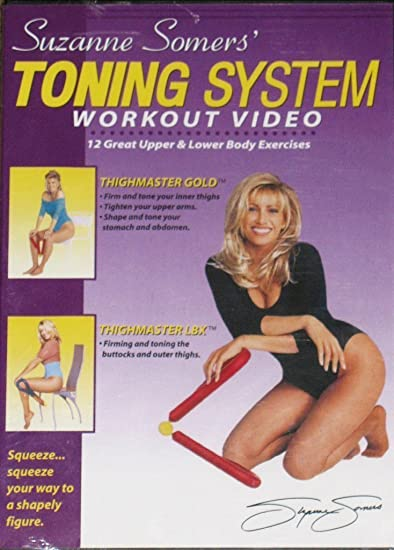
\includegraphics[width=0.3\textwidth,keepaspectratio]{./S01/img/2/suzanne-somers-thighmaster.jpg}
    };
    \draw [white, rounded corners=\ClipSep, line width=\ClipSep]
    (current bounding box.north west) --
    (current bounding box.north east) --
    (current bounding box.south east) --
    (current bounding box.south west) -- cycle
    ;
    \end{tikzpicture}
    \caption{Suzanne Somers - Thighmaster\label{fig:suzanne-somers-thighmaster}}
\end{figure}

\hypertarget{referuxeancias-2}{%
\subsection{Referências}\label{referuxeancias-2}}

\begin{itemize}
\tightlist
\item
  \sloppy Fandom Wiki - Thighmaster. \url{https://threescompany.fandom.com/wiki/Suzanne_Somers#Spokeswoman_for_Thighmaster}
\item
  \sloppy Trechos do comercial - YouTube. \url{https://www.youtube.com/watch?v=2yVeef8AnYI}
\end{itemize}

\hypertarget{in-the-kitchen-with-dinah}{%
\section{In the kitchen with\ldots{}
Dinah?}\label{in-the-kitchen-with-dinah}}

\begin{figure}[!ht]
  \begin{adjustwidth}{-\oddsidemargin-1in}{-\rightmargin}
    \centering
    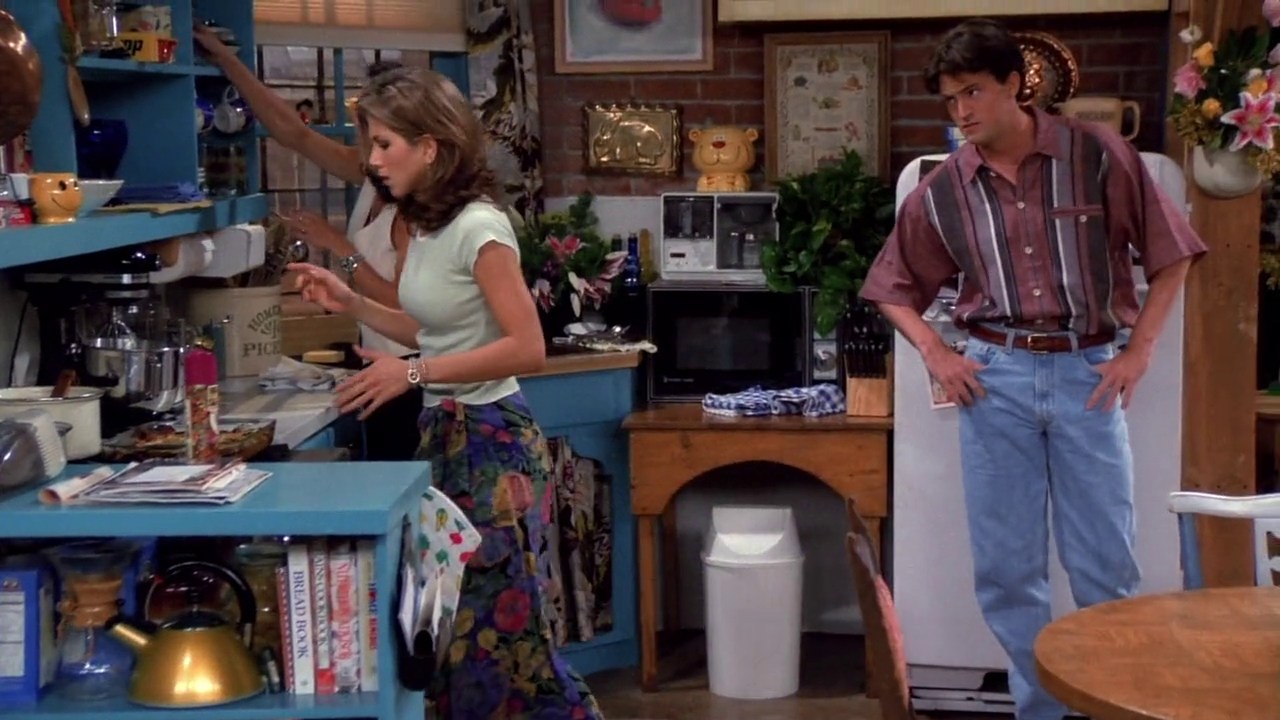
\includegraphics[trim={0 6cm 0 1cm,}, clip, width=\paperwidth]{./S01/img/2/kitchen-with-dinah.png}
    \caption{In the kitchen with… Dinah?\label{fig:in-the-kitchen-with-dinah}}
  \end{adjustwidth}
\end{figure}

\begin{tcolorbox}[enhanced,center upper,
    drop fuzzy shadow southeast, boxrule=0.3pt,
    lower separated=false,
    colframe=black!30!dialogoBorder,colback=white]
\begin{minipage}[c]{0.14\linewidth}
  \raisebox{\dimexpr-\height+\ht\strutbox\relax}{
    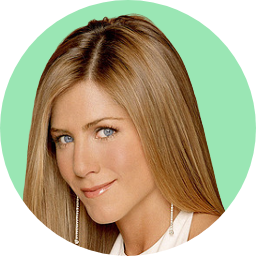
\includegraphics[width=1.5cm]{./assets/img/rachel.png}
  }
   & \centering \scriptsize{Rachel}
\end{minipage}
\hspace{.1mm}
\begin{minipage}[c]{0.8\linewidth}
  \textbf{- I know I had it when I was in the kitchen with...}\\
  - Sei que estava com ela na cozinha com...
\end{minipage}

\medskip
\begin{minipage}[c]{0.14\linewidth}
  \raisebox{\dimexpr-\height+\ht\strutbox\relax}{
    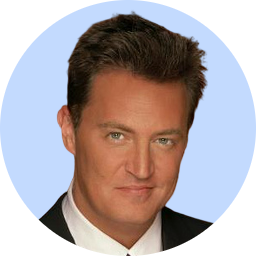
\includegraphics[width=1.5cm]{./assets/img/chandler.png}
  }
   & \centering \scriptsize{Chandler}
\end{minipage}
\hspace{.1mm}
\begin{minipage}[c]{0.8\linewidth}
  \textbf{- Dinah?}\\
  - Dinah?
\end{minipage}
\end{tcolorbox}

Enquanto procura sua aliança, Rachel menciona que estava na cozinha, e
Chandler pergunta se ela estava com Dinah. Isso é uma alusão a canção
folclórica \emph{I've Been Working on the Railroad} (C. 1894). Segue um
trecho da canção que é citado no diálogo:

\bigskip
\begin{tcolorbox}[enhanced,
    drop fuzzy shadow southeast, boxrule=0.3pt,
    lower separated=false, sidebyside, sidebyside align=top,
    halign=flush right, halign lower=left,
    colframe=black!30!dialogoBorder,colback=musicaBg]
\includegraphics[width=0.4cm]{./assets/img/icon-music.png}\\
Someone’s in the kitchen with Dinah\\Someone’s in the kitchen I know\\Someone’s in the kitchen with Dinah\\Strummin’ on the old banjo!\\
\tcblower
\includegraphics[width=0.4cm]{./assets/img/icon-language.png}\\
Alguém está na cozinha com Dinah\\Alguém está na cozinha eu sei\\Alguém está na cozinha com Dinah\\Dedilhando no velho banjo\\
\end{tcolorbox}

\hypertarget{referuxeancias-3}{%
\subsection{Referências}\label{referuxeancias-3}}

\begin{itemize}
\tightlist
\item
  \sloppy Live About - História da música (Inglês). \url{https://www.liveabout.com/ive-been-working-on-the-railroad-traditional-1322525}
\item
  \sloppy Versão por John Denver - YouTube. \url{https://www.youtube.com/watch?v=AAI6wjXEV6g}
\item
  \sloppy Every FRIENDS Joke - Blog. \url{https://every-friends-joke.blogspot.com/2017/06/when-i-was-in-kitchen-with-dinah.html}
\end{itemize}

\hypertarget{minnie-mouse}{%
\section{Minnie Mouse}\label{minnie-mouse}}

\begin{figure}[!ht]
  \begin{adjustwidth}{-\oddsidemargin-1in}{-\rightmargin}
    \centering
    \includegraphics[trim={0 6cm 0 1cm,}, clip, width=\paperwidth]{./S01/img/2/minnie-mouse.png}
    \caption{Minnie Mouse\label{fig:minnie-mouse}}
  \end{adjustwidth}
\end{figure}

\begin{tcolorbox}[enhanced,center upper,
    drop fuzzy shadow southeast, boxrule=0.3pt,
    lower separated=false,
    colframe=black!30!dialogoBorder,colback=white]
\begin{minipage}[c]{0.14\linewidth}
  \raisebox{\dimexpr-\height+\ht\strutbox\relax}{
    \includegraphics[width=1.5cm]{./assets/img/carol-1.png}
  }
   & \centering \scriptsize{Carol}
\end{minipage}
\hspace{.1mm}
\begin{minipage}[c]{0.8\linewidth}
  \textbf{- Minnie, if it's a girl.}\\
  - Minnie, se for menina.
\end{minipage}

\medskip
\begin{minipage}[c]{0.14\linewidth}
  \raisebox{\dimexpr-\height+\ht\strutbox\relax}{
    \includegraphics[width=1.5cm]{./assets/img/ross.png}
  }
   & \centering \scriptsize{Ross}
\end{minipage}
\hspace{.1mm}
\begin{minipage}[c]{0.8\linewidth}
  \textbf{- As in Mouse?}\\
  - Minnie Mouse?
\end{minipage}
\end{tcolorbox}

Ao discutir sobre o nome de seu filho com Carol e Susan, Ross menciona
\emph{Minnie Mouse,} famosa personagem de \emph{Walt Disney} criada em
1928. Aparece pela primeira vez no episódio \emph{Steamboat Willie}
(1928), já como a namorada de \emph{Mickey Mouse}.

\hypertarget{referuxeancias-4}{%
\subsection{Referências}\label{referuxeancias-4}}

\begin{itemize}
\tightlist
\item
  \sloppy Wikipédia. \url{https://pt.wikipedia.org/wiki/Minnie_Mouse}
\item
  \sloppy Steamboat Willie - YouTube. \url{https://www.youtube.com/watch?v=BBgghnQF6E4}
\end{itemize}

\hypertarget{enterprise}{%
\section{Enterprise}\label{enterprise}}

\begin{figure}[!ht]
  \begin{adjustwidth}{-\oddsidemargin-1in}{-\rightmargin}
    \centering
    \includegraphics[trim={0 5cm 0 2cm,}, clip, width=\paperwidth]{./S01/img/2/enterprise.png}
    \caption{Enterprise\label{fig:enterprise}}
  \end{adjustwidth}
\end{figure}

\begin{tcolorbox}[enhanced,center upper,
    drop fuzzy shadow southeast, boxrule=0.3pt,
    lower separated=false,
    colframe=black!30!dialogoBorder,colback=white]
\begin{minipage}[c]{0.14\linewidth}
  \raisebox{\dimexpr-\height+\ht\strutbox\relax}{
    \includegraphics[width=1.5cm]{./assets/img/joey.png}
  }
   & \centering \scriptsize{Joey}
\end{minipage}
\hspace{.1mm}
\begin{minipage}[c]{0.8\linewidth}
  \textbf{- What are we supposed to be seeing here?}\\
  - O que deveríamos ver?
\end{minipage}

\medskip
\begin{minipage}[c]{0.14\linewidth}
  \raisebox{\dimexpr-\height+\ht\strutbox\relax}{
    \includegraphics[width=1.5cm]{./assets/img/chandler.png}
  }
   & \centering \scriptsize{Chandler}
\end{minipage}
\hspace{.1mm}
\begin{minipage}[c]{0.8\linewidth}
  \textbf{- I don't know, but I think it's about to attack the Enterprise.}\\
  - Não sei, mas acho que vai atacar a Enterprise.
\end{minipage}
\end{tcolorbox}

Assistindo ao vídeo do ultrassom, Chandler faz uma piada comparando as
imagens a uma cena da séria \emph{Star Trek} (1966), e \emph{Enterprise}
é o nome da principal nave estelar. No Brasil a séria é conhecido como
\emph{Jornada nas Estrelas}.

\begin{figure}
  \centering
  \begin{tikzpicture}
    \node [inner sep=0pt] at (0,0) {
      \includegraphics[width=0.8\textwidth,keepaspectratio]{./S01/img/2/enterprise-ship.jpg}
    };
    \draw [white, rounded corners=\ClipSep, line width=\ClipSep]
    (current bounding box.north west) --
    (current bounding box.north east) --
    (current bounding box.south east) --
    (current bounding box.south west) -- cycle
    ;
    \end{tikzpicture}
    \caption{Enterprise\label{fig:enterprise}}
\end{figure}

\hypertarget{referuxeancias-5}{%
\subsection{Referências}\label{referuxeancias-5}}

\begin{itemize}
\tightlist
\item
  \sloppy Página oficial. \url{https://intl.startrek.com/database_article/enterprise-nx-01}
\item
  \sloppy Wikipédia. \url{https://pt.wikipedia.org/wiki/USS_Enterprise_(Star_Trek)}
\end{itemize}


\chapter{Aquele com o Dedão}

\textbf{RESUMO $\looparrowright$} Uma empresa de bebidas paga a Phoebe \$ 7.000 depois que ela encontra um dedo numa lata de refrigerante.

\begin{flushright}
\textcolor{gray600}{Exibido em 05 de Outubro de 1994}
\end{flushright}
\hypertarget{laurel-hardy}{%
\section{Laurel \& Hardy}\label{laurel-hardy}}

\begin{figure}[!ht]
  \begin{adjustwidth}{-\oddsidemargin-1in}{-\rightmargin}
    \centering
    \includegraphics[trim={0 7cm 0 2cm,}, clip, width=\paperwidth]{./S01/img/3/laurel-and-hardy.png}
    % \caption{Laurel & Hardy\label{fig:laurel-hardy}}
  \end{adjustwidth}
\end{figure}

No apartamento de Joey e Chandler, enquanto ensaiam para a audição, um
poster de \emph{Laurel \& Hardy} aparece na sala de estar. Esses
personagens são conhecidos no Brasil como \emph{O Gordo e o Magro} e
fizeram cerca de 106 filmes juntos, entre curtas-metragem sonoros e
mudos e filmes.

\hypertarget{referuxeancias}{%
\subsection{Referências}\label{referuxeancias}}

\begin{itemize}
\tightlist
\item
  \sloppy Site oficial. \url{http://www.laurel-and-hardy.com/}
\item
  \sloppy Wikipédia. \url{https://pt.wikipedia.org/wiki/Laurel_%26_Hardy}
\end{itemize}

\hypertarget{grand-jury-secrets}{%
\section{Grand Jury Secrets}\label{grand-jury-secrets}}

\begin{figure}[!ht]
  \begin{adjustwidth}{-\oddsidemargin-1in}{-\rightmargin}
    \centering
    \includegraphics[trim={0 6cm 0 3cm,}, clip, width=\paperwidth]{./S01/img/3/grand-jury-secrets.png}
    % \caption{Grand Jury Secrets\label{fig:grand-jury-secrets}}
  \end{adjustwidth}
\end{figure}

\emph{Grand Jury Secrets} (1939) é um filme de drama e mistério
americano. Conta a história de um repórter inescrupuloso que obtém
notícias através de um rádio escondido na sala de um júri, onde seu
irmão trabalha como advogado. O repórter é sequestrado e escapa devido
sua capacidade de transmitir sua situação.

\begin{figure}
  \centering
  \begin{tikzpicture}
    \node [inner sep=0pt] at (0,0) {
      \includegraphics[width=0.4\textwidth,keepaspectratio]{./S01/img/3/grand-jury-secrets-poster.jpg}
    };
    \draw [white, rounded corners=\ClipSep, line width=\ClipSep]
    (current bounding box.north west) --
    (current bounding box.north east) --
    (current bounding box.south east) --
    (current bounding box.south west) -- cycle
    ;
    \end{tikzpicture}
    \caption{Grand Jury Secrets poster\label{fig:grand-jury-secrets-poster}}
\end{figure}

\hypertarget{referuxeancias-1}{%
\subsection{Referências}\label{referuxeancias-1}}

\begin{itemize}
\tightlist
\item
  \sloppy BFI. \url{https://www.bfi.org.uk/films-tv-people/4ce2b6ab720c8}
\item
  \sloppy Loving The Classics. \url{https://www.lovingtheclassics.com/by-title/g/grand-jury-secrets-1939.html}
\item
  \sloppy IMDB. \url{https://www.imdb.com/title/tt0031390/}
\end{itemize}

\hypertarget{there-was-a-crooked-man}{%
\section{There was a crooked
man\ldots{}}\label{there-was-a-crooked-man}}

\begin{figure}[!ht]
  \begin{adjustwidth}{-\oddsidemargin-1in}{-\rightmargin}
    \centering
    \includegraphics[trim={0 7cm 0 2cm,}, clip, width=\paperwidth]{./S01/img/3/crooked-man.png}
    % \caption{There was a crooked man\label{fig:there-was-a-crooked-man}}
  \end{adjustwidth}
\end{figure}

\begin{tcolorbox}[enhanced,center upper,
    drop fuzzy shadow southeast, boxrule=0.3pt,
    lower separated=false,
    colframe=black!30!dialogoBorder,colback=white]
\begin{minipage}[c]{0.16\linewidth}
  \raisebox{\dimexpr-\height+\ht\strutbox\relax}{
    \centering \includegraphics[width=1.4cm]{./assets/img/phoebe.png}
  }
   & \centering \scriptsize{Phoebe}
\end{minipage}
\hfill
\begin{minipage}[c]{0.8\linewidth}
  \textbf{- From the nursery rhyme. 'There was a crooked man, Who had a crooked smile, Who lived in a shoe, For a... while...'}\\
  - Da musiquinha. 'Havia um cara de sorriso torto. E morava no sapato, por um... tempo...
\end{minipage}
\end{tcolorbox}

Enquanto os amigos discutem o quanto Alan é legal, Phoebe o compara com
o homem no sapato, que, como Joey notou, tem um sorisso torto. A
``musiquinha'' ou canção de ninar é \emph{There Was a Crooked Man} (C.
1840) de origem desconhecida.

Letra original e tradução da canção:

\bigskip
\begin{tcolorbox}[enhanced,
    drop fuzzy shadow southeast, boxrule=0.3pt,
    lower separated=false, sidebyside, sidebyside align=top,
    halign=flush right, halign lower=left,
    colframe=black!30!dialogoBorder,colback=musicaBg]
\includegraphics[width=0.4cm]{./assets/img/icon-music.png}\\
There was a crooked man, and he walked a crooked mile.\\He found a crooked sixpence upon a crooked stile.\\He bought a crooked cat, which caught a crooked mouse,\\And they all lived together in a little crooked house.\\
\tcblower
\includegraphics[width=0.4cm]{./assets/img/icon-language.png}\\
Havia um homem torto, e ele andou em uma estrada torta\\Ele encontrou uma moeda torta sobre um rebordo torto\\Ele comprou um gato torto, que pegou um rato torto\\E eles todos viveram juntos em uma pequena casa torta\\
\end{tcolorbox}

\hypertarget{referuxeancias-2}{%
\subsection{Referências}\label{referuxeancias-2}}

\begin{itemize}
\tightlist
\item
  \sloppy Wikipédia. \url{https://en.wikipedia.org/wiki/There_Was_a_Crooked_Man}
\item
  \sloppy There Was A Crooked Man Nursery Rhyme - YouTube. \url{https://www.youtube.com/watch?v=WqyUOlz_6i4}
\item
  Alchin, Linda Kathryn. \emph{Secret History of Nursery Rhymes.} Linda
  Alchin, 2010.
\end{itemize}

\hypertarget{david-hasselhoff}{%
\section{David Hasselhoff}\label{david-hasselhoff}}

\begin{figure}[!ht]
  \begin{adjustwidth}{-\oddsidemargin-1in}{-\rightmargin}
    \centering
    \includegraphics[trim={0 6cm 0 2cm,}, clip, width=\paperwidth]{./S01/img/3/david-hasselhoff.png}
    % \caption{David Hasselhoff\label{fig:david-hasselhoff}}
  \end{adjustwidth}
\end{figure}

\begin{tcolorbox}[enhanced,center upper,
    drop fuzzy shadow southeast, boxrule=0.3pt,
    lower separated=false,
    colframe=black!30!dialogoBorder,colback=white]
\begin{minipage}[c]{0.16\linewidth}
  \raisebox{\dimexpr-\height+\ht\strutbox\relax}{
    \centering \includegraphics[width=1.4cm]{./assets/img/chandler.png}
  }
   & \centering \scriptsize{Chandler}
\end{minipage}
\hfill
\begin{minipage}[c]{0.8\linewidth}
  \textbf{- I'd marry him just for his David Hasselhoff impression alone.}\\
  - Eu casaria por causa da imitação de David Hasselholff.
\end{minipage}
\end{tcolorbox}

\emph{David Hasselhoff} é ator, cantor, produtor e empresário
norte-americano. Um de seus grandes papeis de sucesso foi o salva-vidas
\emph{Mitch Buchannon} em \emph{Baywatch} (1989 - 2001), conhecida no
Brasil como \emph{S.O.S. Malibu}, série que acaba sendo conhecida como a
preferida de Joey no episódio
\textbf{\textcolor{primarycolor}{S03E06 - Aquele do flashback}}, em que
ele apresenta a série a Chandler.

\begin{figure}
  \centering
  \begin{tikzpicture}
    \node [inner sep=0pt] at (0,0) {
      \includegraphics[width=0.8\textwidth,keepaspectratio]{./S01/img/3/david-hasselhoff-baywatch.jpg}
    };
    \draw [white, rounded corners=\ClipSep, line width=\ClipSep]
    (current bounding box.north west) --
    (current bounding box.north east) --
    (current bounding box.south east) --
    (current bounding box.south west) -- cycle
    ;
    \end{tikzpicture}
    \caption{David Hasselhoff em Baywatch\label{fig:david-hasselhoff-em-baywatch}}
\end{figure}

\hypertarget{referuxeancias-3}{%
\subsection{Referências}\label{referuxeancias-3}}

\begin{itemize}
\tightlist
\item
  \sloppy IMDB. \url{https://www.imdb.com/name/nm0001327/}
\item
  \sloppy Site oficial Baywatch. \url{https://www.baywatch.com/}
\end{itemize}

\hypertarget{bugs-bunny}{%
\section{Bugs Bunny}\label{bugs-bunny}}

\begin{figure}[!ht]
  \begin{adjustwidth}{-\oddsidemargin-1in}{-\rightmargin}
    \centering
    \includegraphics[trim={0 7cm 0 2cm,}, clip, width=\paperwidth]{./S01/img/3/bugs-bunny.png}
    % \caption{Bugs Bunny\label{fig:bugs-bunny}}
  \end{adjustwidth}
\end{figure}

\begin{tcolorbox}[enhanced,center upper,
    drop fuzzy shadow southeast, boxrule=0.3pt,
    lower separated=false,
    colframe=black!30!dialogoBorder,colback=white]
\begin{minipage}[c]{0.16\linewidth}
  \raisebox{\dimexpr-\height+\ht\strutbox\relax}{
    \centering \includegraphics[width=1.4cm]{./assets/img/ross.png}
  }
   & \centering \scriptsize{Ross}
\end{minipage}
\hfill
\begin{minipage}[c]{0.8\linewidth}
  \textbf{- He was like that Bugs Bunny cartoon where Bugs is playing all the positions.}\\
  - Ele parecia o Pernalonga no desenho em que jogava em todas as posições.
\end{minipage}
\end{tcolorbox}

Enquanto explica como Alan joga bem \emph{softball}, Ross menciona
\emph{Bugs Bunny}, conhecido no Brasil como \emph{Pernalonga},
personagem da \emph{Looney Tunes}. O episódio citado por Ross é o
\emph{Baseball Bugs} (1946).

\begin{figure}
  \centering
  \begin{tikzpicture}
    \node [inner sep=0pt] at (0,0) {
      \includegraphics[width=0.4\textwidth,keepaspectratio]{./S01/img/3/baseball-bugs.jpg}
    };
    \draw [white, rounded corners=\ClipSep, line width=\ClipSep]
    (current bounding box.north west) --
    (current bounding box.north east) --
    (current bounding box.south east) --
    (current bounding box.south west) -- cycle
    ;
    \end{tikzpicture}
    \caption{Baseball Bugs\label{fig:baseball-bugs}}
\end{figure}

\hypertarget{referuxeancias-4}{%
\subsection{Referências}\label{referuxeancias-4}}

\begin{itemize}
\tightlist
\item
  \sloppy Fandom Wiki - Looney Tunes. \url{https://looneytunes.fandom.com/wiki/Baseball_Bugs}
\item
  \sloppy IMDB. \url{https://www.imdb.com/title/tt0038333/}
\item
  \sloppy Episódio na SuperCartoons (Inglês). \url{https://www.supercartoons.net/cartoon/629/bugs-bunny-baseball-bugs.html}
\item
  \sloppy Diferenças entre softball e baseball (Inglês). \url{https://www.dummies.com/sports/fantasy-sports/fantasy-baseball/the-differences-between-softball-and-baseball/}
\end{itemize}

\hypertarget{lamb-chop}{%
\section{Lamb Chop}\label{lamb-chop}}

\begin{figure}[!ht]
  \begin{adjustwidth}{-\oddsidemargin-1in}{-\rightmargin}
    \centering
    \includegraphics[trim={0 6cm 0 3cm,}, clip, width=\paperwidth]{./S01/img/3/lamb-chop.png}
    % \caption{Lamb Chop\label{fig:lamb-chop}}
  \end{adjustwidth}
\end{figure}

\begin{tcolorbox}[enhanced,center upper,
    drop fuzzy shadow southeast, boxrule=0.3pt,
    lower separated=false,
    colframe=black!30!dialogoBorder,colback=white]
\begin{minipage}[c]{0.16\linewidth}
  \raisebox{\dimexpr-\height+\ht\strutbox\relax}{
    \centering \includegraphics[width=1.4cm]{./assets/img/chandler.png}
  }
   & \centering \scriptsize{Chandler}
\end{minipage}
\hfill
\begin{minipage}[c]{0.8\linewidth}
  \textbf{- If I had a sock on my hand for 30 years, it'd be talking too.}\\
  - Se eu usasse uma meia na mão por 30 anos, ela também ia falar.
\end{minipage}
\end{tcolorbox}

No apartamento de Monica os amigos assistem a \emph{Lamb Chop}, fantoche
criado por \emph{Shari Lewis} (1934-1998). Sua filha, \emph{Mallory
Lewis}, continuou seu legado e faz performances de \emph{Lamb Chop} até
hoje.

\begin{figure}
  \centering
  \begin{tikzpicture}
    \node [inner sep=0pt] at (0,0) {
      \includegraphics[width=0.7\textwidth,keepaspectratio]{./S01/img/3/shari-lewis.jpg}
    };
    \draw [white, rounded corners=\ClipSep, line width=\ClipSep]
    (current bounding box.north west) --
    (current bounding box.north east) --
    (current bounding box.south east) --
    (current bounding box.south west) -- cycle
    ;
    \end{tikzpicture}
    \caption{Shari Lewis\label{fig:shari-lewis}}
\end{figure}

\hypertarget{referuxeancias-5}{%
\subsection{Referências}\label{referuxeancias-5}}

\begin{itemize}
\tightlist
\item
  \sloppy Site oficial. \url{https://mallorylewisandlambchop.com/faqs/}
\end{itemize}


\chapter{Aquele com George Stephanopoulus}

\textbf{RESUMO $\looparrowright$} Um entregador acidentalmente leva uma pizza que deveria ser entregue a George Stephanopoulos, que mora em frente às meninas.

\begin{flushright}
\textcolor{gray600}{Exibido em 12 de Outubro de 1994}
\end{flushright}
\hypertarget{dairy-queen}{%
\section{Dairy Queen}\label{dairy-queen}}

\begin{figure}[!ht]
  \begin{adjustwidth}{-\oddsidemargin-1in}{-\rightmargin}
    \centering
    \includegraphics[trim={0 7cm 0 2cm,}, clip, width=\paperwidth]{./S01/img/4/dairy-queen.png}
    % \caption{Dairy Queen\label{fig:dairy-queen}}
  \end{adjustwidth}
\end{figure}

\begin{tcolorbox}[enhanced,center upper,
    drop fuzzy shadow southeast, boxrule=0.3pt,
    lower separated=false, breakable,
    colframe=black!30!dialogoBorder,colback=white]
\begin{minipage}[c]{0.16\linewidth}
  \raisebox{\dimexpr-\height+\ht\strutbox\relax}{
    \centering \includegraphics[width=1.4cm]{./assets/img/phoebe.png}
  }
   & \centering \scriptsize{Phoebe}
\end{minipage}
\hfill
\begin{minipage}[c]{0.8\linewidth}
  \textbf{- There was a cave-in in one of the mines, and eight people were killed.}\\
  - Uma mina desabou e oito pessoas morreram.
\end{minipage}

\medskip
\begin{minipage}[c]{0.16\linewidth}
  \raisebox{\dimexpr-\height+\ht\strutbox\relax}{
    \centering \includegraphics[width=1.4cm]{./assets/img/monica.png}
  }
   & \centering \scriptsize{Monica}
\end{minipage}
\hfill
\begin{minipage}[c]{0.8\linewidth}
  \textbf{- Wow, you worked in a mine?}\\
  - Trabalhou em uma mina?
\end{minipage}

\medskip
\begin{minipage}[c]{0.16\linewidth}
  \raisebox{\dimexpr-\height+\ht\strutbox\relax}{
    \centering \includegraphics[width=1.4cm]{./assets/img/phoebe.png}
  }
   & \centering \scriptsize{Phoebe}
\end{minipage}
\hfill
\begin{minipage}[c]{0.8\linewidth}
  \textbf{- No, I worked at a Dairy Queen. Why?}\\
  - Não, em um Dairy Queen. Por quê?
\end{minipage}
\end{tcolorbox}

Enquanto discutem sobre empregos e salários, Phoebe menciona um de seus
empregos em uma mina. Monica fica abismada com o fato e quer saber se
aquilo era verdade. Phoebe, sarcasticamente, responde que não, na
verdade era um \emph{Dairy Queen}. \footnote{\sloppy Site oficial. \url{https://dairyqueen.com/}}

\emph{Dairy Queen} (1940) é uma famosa rede de sorveterias e
restaurantes de \emph{fast-food}.

\hypertarget{rachel-has-left-the-building}{%
\section{Rachel has left the
building}\label{rachel-has-left-the-building}}

\begin{figure}[!ht]
  \begin{adjustwidth}{-\oddsidemargin-1in}{-\rightmargin}
    \centering
    \includegraphics[trim={0 6cm 0 2cm,}, clip, width=\paperwidth]{./S01/img/4/rachel-has-left-the-building.png}
    % \caption{Rachel has left the building\label{fig:rachel-has-left-the-building}}
  \end{adjustwidth}
\end{figure}

\begin{tcolorbox}[enhanced,center upper,
    drop fuzzy shadow southeast, boxrule=0.3pt,
    lower separated=false, breakable,
    colframe=black!30!dialogoBorder,colback=white]
\begin{minipage}[c]{0.16\linewidth}
  \raisebox{\dimexpr-\height+\ht\strutbox\relax}{
    \centering \includegraphics[width=1.4cm]{./assets/img/monica.png}
  }
   & \centering \scriptsize{Monica}
\end{minipage}
\hfill
\begin{minipage}[c]{0.8\linewidth}
  \textbf{- Rachel has left the building.}\\
  - Rachel deixou o edifício.
\end{minipage}
\end{tcolorbox}

Após atender a um telefonema da operadora de cartão perguntando sobre a
Rachel, Monica diz a frase \emph{Rachel has left the building}. Isto é
uma paráfrase de \emph{Elvis has left the building}. Era uma frase usada
para dispersar o público que ficava a espera do bis ao final do show do
Rei do \emph{Rock and Roll Elvis Presley}. \footnote{\sloppy Fandom Wiki. \url{https://friends.fandom.com/wiki/The_One_With_George_Stephanopoulos}}
\footnote{\sloppy Wikipédia. \url{https://en.wikipedia.org/wiki/Elvis_has_left_the_building}}

\hypertarget{jack-and-the-beanstalk}{%
\section{Jack and the Beanstalk}\label{jack-and-the-beanstalk}}

\begin{figure}[!ht]
  \begin{adjustwidth}{-\oddsidemargin-1in}{-\rightmargin}
    \centering
    \includegraphics[trim={0 6cm 0 2cm,}, clip, width=\paperwidth]{./S01/img/4/jack-and-the-beanstalk.png}
    % \caption{Jack and the Beanstalk\label{fig:jack-and-the-beanstalk}}
  \end{adjustwidth}
\end{figure}

\begin{tcolorbox}[enhanced,center upper,
    drop fuzzy shadow southeast, boxrule=0.3pt,
    lower separated=false, breakable,
    colframe=black!30!dialogoBorder,colback=white]
\begin{minipage}[c]{0.16\linewidth}
  \raisebox{\dimexpr-\height+\ht\strutbox\relax}{
    \centering \includegraphics[width=1.4cm]{./assets/img/phoebe.png}
  }
   & \centering \scriptsize{Phoebe}
\end{minipage}
\hfill
\begin{minipage}[c]{0.8\linewidth}
  \textbf{- You are just like Jack.}\\
  - Você é igual ao João.
\end{minipage}

\medskip
\begin{minipage}[c]{0.16\linewidth}
  \raisebox{\dimexpr-\height+\ht\strutbox\relax}{
    \centering \includegraphics[width=1.4cm]{./assets/img/rachel.png}
  }
   & \centering \scriptsize{Rachel}
\end{minipage}
\hfill
\begin{minipage}[c]{0.8\linewidth}
  \textbf{- Jack from downstairs?}\\
  - João, do andar de baixo?
\end{minipage}

\medskip
\begin{minipage}[c]{0.16\linewidth}
  \raisebox{\dimexpr-\height+\ht\strutbox\relax}{
    \centering \includegraphics[width=1.4cm]{./assets/img/phoebe.png}
  }
   & \centering \scriptsize{Phoebe}
\end{minipage}
\hfill
\begin{minipage}[c]{0.8\linewidth}
  \textbf{- No, Jack and the Beanstalk.}\\
  - Não, João e o Pé de Feijão.
\end{minipage}
\end{tcolorbox}

\emph{Jack and the Beanstalk} (1807), conhecido no Brasil como
\emph{João e o Pé de Feijão}, é um conto de fadas de origem inglesa. A
Phoebe conta bem o enredo da história na cena. É uma história bastante
conhecida e referenciada diversas vezes, como em \emph{O Pica-pau},
\emph{Mickey Mouse}, entre outros.\footnote{\sloppy Página da Universidade de Pittsburgh (Inglês). \url{https://www.pitt.edu/~dash/type0328jack.html}}

\hypertarget{george-stephanopoulos}{%
\section{George Stephanopoulos}\label{george-stephanopoulos}}

\begin{figure}[!ht]
  \begin{adjustwidth}{-\oddsidemargin-1in}{-\rightmargin}
    \centering
    \includegraphics[trim={0 10cm 0 3cm,}, clip, width=\paperwidth]{./S01/img/4/george-stephanopoulos.png}
    % \caption{George Stephanopoulos\label{fig:george-stephanopoulos}}
  \end{adjustwidth}
\end{figure}

\begin{tcolorbox}[enhanced,center upper,
    drop fuzzy shadow southeast, boxrule=0.3pt,
    lower separated=false, breakable,
    colframe=black!30!dialogoBorder,colback=white]
\begin{minipage}[c]{0.16\linewidth}
  \raisebox{\dimexpr-\height+\ht\strutbox\relax}{
    \centering \includegraphics[width=1.4cm]{./assets/img/monica.png}
  }
   & \centering \scriptsize{Monica}
\end{minipage}
\hfill
\begin{minipage}[c]{0.8\linewidth}
  \textbf{- Did you say G. Stephanopoulos?}\\
  - Calma, você falou G. Stephanopoulos?
\end{minipage}
\end{tcolorbox}

\emph{George Stephanopoulos} (1961-) \footnote{\sloppy Twitter. \url{https://twitter.com/gstephanopoulos}}
realmente existe e na época dessa temporada era diretor de comunicações
da campanha presidencial de Bill Clinton. Atualmente é, entre outras
coisas, âncora do telejornal \emph{Good Morning America}.\footnote{\sloppy IMDB. \url{https://www.imdb.com/name/nm0826888/?ref_=tt_ov_st_sm}}

Essa passagem de sua vida virou o documentário \emph{The War Room}
(1993).\footnote{\sloppy IMDB Documentário. \url{https://www.imdb.com/title/tt0108515/}}

\begin{figure}
  \centering
  \begin{tikzpicture}
    \node [inner sep=0pt] at (0,0) {
      \includegraphics[width=0.6\textwidth,keepaspectratio]{./S01/img/4/george-stephanopoulos-war-room.jpg}
    };
    \draw [white, rounded corners=\ClipSep, line width=\ClipSep]
    (current bounding box.north west) --
    (current bounding box.north east) --
    (current bounding box.south east) --
    (current bounding box.south west) -- cycle
    ;
    \end{tikzpicture}
    \caption{George Stephanopoulos - The War Room\label{fig:george-stephanopoulos-the-war-room}}
\end{figure}

\hypertarget{george-snuffleupagus}{%
\section{George ``Snuffleupagus''}\label{george-snuffleupagus}}

\begin{figure}[!ht]
  \begin{adjustwidth}{-\oddsidemargin-1in}{-\rightmargin}
    \centering
    \includegraphics[trim={0 8cm 0 1cm,}, clip, width=\paperwidth]{./S01/img/4/george-snuffleupagus.png}
    % \caption{George ``Snuffleupagus''\label{fig:george-snuffleupagus}}
  \end{adjustwidth}
\end{figure}

\begin{tcolorbox}[enhanced,center upper,
    drop fuzzy shadow southeast, boxrule=0.3pt,
    lower separated=false, breakable,
    colframe=black!30!dialogoBorder,colback=white]
\begin{minipage}[c]{0.16\linewidth}
  \raisebox{\dimexpr-\height+\ht\strutbox\relax}{
    \centering \includegraphics[width=1.4cm]{./assets/img/rachel.png}
  }
   & \centering \scriptsize{Rachel}
\end{minipage}
\hfill
\begin{minipage}[c]{0.8\linewidth}
  \textbf{- Who's George Snuffleupagus?}\\
  - Quem é George Snuffleupagus?
\end{minipage}

\medskip
\begin{minipage}[c]{0.16\linewidth}
  \raisebox{\dimexpr-\height+\ht\strutbox\relax}{
    \centering \includegraphics[width=1.4cm]{./assets/img/phoebe.png}
  }
   & \centering \scriptsize{Phoebe}
\end{minipage}
\hfill
\begin{minipage}[c]{0.8\linewidth}
  \textbf{- That's Big Bird's friend.}\\
  - Amigo do Garibaldo.
\end{minipage}
\end{tcolorbox}

Rachel confunde o sobrenome de George e o chama de \emph{Snuffleupagus}
\footnote{\sloppy Fandom Wiki - Mr. Snuffleupagus. \url{https://muppet.fandom.com/wiki/Mr._Snuffleupagus}}.
Ele é realmente amigo de \emph{Big Bird} \footnote{\sloppy Fandom Wiki - Big Bird. \url{https://muppet.fandom.com/wiki/Big_Bird}}
e, ambos, fazem parte do programa de televisão educacional \emph{Sesame
Street} (1969), conhecido no Brasil como \emph{Vila Sésamo} \footnote{\sloppy Sesame Street - Site oficial. \url{https://www.sesamestreet.org/}}.
Em nossa versão, \emph{Snuffleupagus} era \emph{Funga-Funga} (à direita)
e \emph{Big Bird} era \emph{Garibaldo} (à esquerda).

\begin{figure}
  \centering
  \begin{tikzpicture}
    \node [inner sep=0pt] at (0,0) {
      \includegraphics[width=0.5\textwidth,keepaspectratio]{./S01/img/4/snuffleupagus-big-bird.jpg}
    };
    \draw [white, rounded corners=\ClipSep, line width=\ClipSep]
    (current bounding box.north west) --
    (current bounding box.north east) --
    (current bounding box.south east) --
    (current bounding box.south west) -- cycle
    ;
    \end{tikzpicture}
    \caption{Snuffleupagus e Big Bird\label{fig:snuffleupagus-e-big-bird}}
\end{figure}

\hypertarget{silence-of-the-lambs}{%
\section{Silence of the Lambs}\label{silence-of-the-lambs}}

\begin{figure}[!ht]
  \begin{adjustwidth}{-\oddsidemargin-1in}{-\rightmargin}
    \centering
    \includegraphics[trim={0 8cm 0 3cm,}, clip, width=\paperwidth]{./S01/img/4/silence-of-the-lambs.png}
    % \caption{Silence of the Lambs\label{fig:silence-of-the-lambs}}
  \end{adjustwidth}
\end{figure}

\begin{tcolorbox}[enhanced,center upper,
    drop fuzzy shadow southeast, boxrule=0.3pt,
    lower separated=false, breakable,
    colframe=black!30!dialogoBorder,colback=white]
\begin{minipage}[c]{0.16\linewidth}
  \raisebox{\dimexpr-\height+\ht\strutbox\relax}{
    \centering \includegraphics[width=1.4cm]{./assets/img/chandler.png}
  }
   & \centering \scriptsize{Chandler}
\end{minipage}
\hfill
\begin{minipage}[c]{0.8\linewidth}
  \textbf{- Oh, I thought you were great in Silence of the Lambs.}\\
  - Você estava ótimo em Silêncio dos Inocentes.
\end{minipage}
\end{tcolorbox}

\emph{Silence of the Lambs} (1991) é um filme norte-americano de
suspense, drama e terror, estrelado por \emph{Jodie Foster} e
\emph{Anthony Hopkins}. A comparação feita por Chandler se refere ao
modo como o \emph{Dr.~Hannibal Lecter}, interpretado por \emph{Hopkins},
era transportado quando precisava sair da cadeia. No Brasil o filme
ficou conhecido como \emph{Silêncio dos Inocentes}.\footnote{\sloppy The Silence of the Lambs - IMDB. \url{https://www.imdb.com/title/tt0102926/}}

\begin{figure}
  \centering
  \begin{tikzpicture}
    \node [inner sep=0pt] at (0,0) {
      \includegraphics[width=0.5\textwidth,keepaspectratio]{./S01/img/4/hannibal-lecter.jpg}
    };
    \draw [white, rounded corners=\ClipSep, line width=\ClipSep]
    (current bounding box.north west) --
    (current bounding box.north east) --
    (current bounding box.south east) --
    (current bounding box.south west) -- cycle
    ;
    \end{tikzpicture}
    \caption{Hannibal Lecter\label{fig:hannibal-lecter}}
\end{figure}


\chapter{Aquele com o Sabão em Pó da Alemanha Oriental}

\textbf{RESUMO $\looparrowright$} Ross ajuda Rachel a lavar a roupa e considera o evento um primeiro encontro. Joey faz com que Monica se passe como sua nova namorada.

\begin{flushright}
\textcolor{gray600}{Exibido em 19 de Outubro de 1994}
\end{flushright}
\hypertarget{bullwinkle-socks}{%
\section{Bullwinkle socks}\label{bullwinkle-socks}}

\begin{figure}[!ht]
  \begin{adjustwidth}{-\oddsidemargin-1in}{-\rightmargin}
    \centering
    \includegraphics[trim={0 4cm 0 3cm,}, clip, width=\paperwidth]{./S01/img/5/bullwinkle-socks.png}
    % \caption{Bullwinkle socks\label{fig:bullwinkle-socks}}
  \end{adjustwidth}
\end{figure}

\begin{tcolorbox}[enhanced,center upper,
    drop fuzzy shadow southeast, boxrule=0.3pt,
    lower separated=false, breakable,
    colframe=black!30!dialogoBorder,colback=white]
\begin{minipage}[c]{0.16\linewidth}
  \raisebox{\dimexpr-\height+\ht\strutbox\relax}{
    \centering \includegraphics[width=1.4cm]{./assets/img/janice.png}
  }
   & \centering \scriptsize{Janice}
\end{minipage}
\hfill
\begin{minipage}[c]{0.8\linewidth}
  \textbf{- I got you... these.}\\
  - Comprei... isto.
\end{minipage}

\medskip
\begin{minipage}[c]{0.16\linewidth}
  \raisebox{\dimexpr-\height+\ht\strutbox\relax}{
    \centering \includegraphics[width=1.4cm]{./assets/img/chandler.png}
  }
   & \centering \scriptsize{Chandler}
\end{minipage}
\hfill
\begin{minipage}[c]{0.8\linewidth}
  \textbf{- Bullwinkle socks.}\\
  - Uma meia do Alceu.
\end{minipage}
\end{tcolorbox}

\saveparinfos
\noindent
\begin{minipage}[c]{0.5\textwidth}\useparinfo

Para o dia dos namorados, Janice compra para Chandler meias do
\emph{Bullwinkle}, personagem de desenho animado, que junto com
\emph{Rocky}, estrelavam o programa \emph{The Rocky and Bullwinkle Show}
(1959). No Brasil a dupla ficou conhecida como Alceu (\emph{Bullwinkle})
e Dentinho (\emph{Rocky}).\footnote{\sloppy Bullwinkle - Fandom Wiki (Inglês). \url{https://rockyandbullwinkle.fandom.com/wiki/Bullwinkle_J._Moose}}

\end{minipage}\hfill
\begin{minipage}[c]{0.5\textwidth}

\begin{figure}
  \centering
  \begin{tikzpicture}
    \node [inner sep=0pt] at (0,0) {
      \includegraphics[width=0.8\textwidth,keepaspectratio]{./S01/img/5/rocky-bullwinkle.jpg}
    };
    \draw [white, rounded corners=\ClipSep, line width=\ClipSep]
    (current bounding box.north west) --
    (current bounding box.north east) --
    (current bounding box.south east) --
    (current bounding box.south west) -- cycle
    ;
    \end{tikzpicture}
    \caption{Rocky and Bullwinkle\label{fig:rocky-and-bullwinkle}}
\end{figure}

\end{minipage}

\hypertarget{underdog}{%
\section{Underdog}\label{underdog}}

\begin{figure}[!ht]
  \begin{adjustwidth}{-\oddsidemargin-1in}{-\rightmargin}
    \centering
    \includegraphics[trim={0 6.5cm 0 2.5cm,}, clip, width=\paperwidth]{./S01/img/5/underdog.png}
    % \caption{Underdog\label{fig:underdog}}
  \end{adjustwidth}
\end{figure}

\begin{tcolorbox}[enhanced,center upper,
    drop fuzzy shadow southeast, boxrule=0.3pt,
    lower separated=false,
    colframe=black!30!dialogoBorder,colback=white]
\begin{minipage}[c]{0.16\linewidth}
  \raisebox{\dimexpr-\height+\ht\strutbox\relax}{
    \centering \includegraphics[width=1.4cm]{./assets/img/monica.png}
  }
   & \centering \scriptsize{Monica}
\end{minipage}
\hfill
\begin{minipage}[c]{0.8\linewidth}
  \textbf{- Something went wrong with Underdog, and they couldn't get his head to inflate.}\\
  - Aconteceu algo com o Vira-lata. E a cabeça dele não inflava.
\end{minipage}
\end{tcolorbox}

No ``encontro duplo'', Monica menciona o \emph{Underdog} (1964)
\footnote{\sloppy Underdog - IMDB. \url{https://www.imdb.com/title/tt0060037/}},
desenho animado americano protagonizado por um cão super-herói. O
interessante dessa cena é que Monica menciona algo que só vai ocorrer no
episódio
\textbf{\textcolor{primarycolor}{S01E09 - Aquele em que o Underdog Escapa}},
quatro episódios mais tarde.

\begin{figure}
  \centering
  \begin{tikzpicture}
    \node [inner sep=0pt] at (0,0) {
      \includegraphics[width=0.7\textwidth,keepaspectratio]{./S01/img/5/underdog-s01e09.png}
    };
    \draw [white, rounded corners=\ClipSep, line width=\ClipSep]
    (current bounding box.north west) --
    (current bounding box.north east) --
    (current bounding box.south east) --
    (current bounding box.south west) -- cycle
    ;
    \end{tikzpicture}
    \caption{S01E09 - Aquele em que o Underdog Escapa\label{fig:s01-e09-aquele-em-que-o-underdog-escapa}}
\end{figure}

\hypertarget{cocktails-in-appalachia}{%
\section{Cocktails in Appalachia}\label{cocktails-in-appalachia}}

\begin{figure}[!ht]
  \begin{adjustwidth}{-\oddsidemargin-1in}{-\rightmargin}
    \centering
    \includegraphics[trim={0 7cm 0 1cm,}, clip, width=\paperwidth]{./S01/img/5/cocktails-in-appalachia.png}
    % \caption{Cocktails in Appalachia\label{fig:cocktails-in-appalachia}}
  \end{adjustwidth}
\end{figure}

\begin{tcolorbox}[enhanced,center upper,
    drop fuzzy shadow southeast, boxrule=0.3pt,
    lower separated=false, breakable,
    colframe=black!30!dialogoBorder,colback=white]
\begin{minipage}[c]{0.16\linewidth}
  \raisebox{\dimexpr-\height+\ht\strutbox\relax}{
    \centering \includegraphics[width=1.4cm]{./assets/img/monica.png}
  }
   & \centering \scriptsize{Monica}
\end{minipage}
\hfill
\begin{minipage}[c]{0.8\linewidth}
  \textbf{- Hello! Were we at the same table? It's like... Cocktails in Appalachia.}\\
  - Estamos na mesma mesa? Os dois estão pegando fogo!
\end{minipage}
\end{tcolorbox}

Abismada com o fato de Bob e Angela estarem se pegando, Monica menciona
que aquilo parecia \emph{Cocktails in Appalachia}. \emph{Appalachia} é
uma cidade do estado da Virgínia. O termo refere-se a esteriótipos do
local, que incluem incesto. Daí o termo usado por Monica, já que ela
pensa que os dois são irmãos.\footnote{\sloppy MD Recruits Face Culture Shock in Appalachia - ABS News (Inglês). \url{https://abcnews.go.com/Health/story?id=5922943\&page=1}}


\chapter{Aquele com o Traseiro}

\textbf{RESUMO $\looparrowright$} Aparece a grande oportunidade de Joey: ele é contratado para ser dublê de Al Pacino.

\begin{flushright}
\textcolor{gray600}{Exibido em 26 de Outubro de 1994}
\end{flushright}
\hypertarget{freud}{%
\section{Freud!}\label{freud}}

\begin{figure}[!ht]
  \begin{adjustwidth}{-\oddsidemargin-1in}{-\rightmargin}
    \centering
    \includegraphics[trim={0 7cm 0 3cm,}, clip, width=\paperwidth]{./S01/img/6/freud.png}
    % \caption{Freud\label{fig:freud}}
  \end{adjustwidth}
\end{figure}

Joey é o protagonista do musical \emph{Freud!}, atuando como
\emph{Sigmund Freud} (1856), considerado o Pai da Psicanálise. No
musical, Joey canta uma música sobre um assunto abordado no livro de
Freud chamado \emph{The Psychical Consequences of the Anatomic
Distinction Between the Sexes} (1925), onde ele explica algo que ficou
conhecido como `Penis Envy' (Inveja do pênis).

\begin{quote}
All you want is a dinkle
\end{quote}

\begin{quote}
What you envy's a schwang
\end{quote}

\begin{quote}
A thing through which you can tinkle
\end{quote}

\begin{quote}
To play with or simply let hang
\end{quote}

Na letra, \emph{dinkle} e \emph{schwang} são metáforas para pênis.

\hypertarget{referuxeancias}{%
\subsection{Referências}\label{referuxeancias}}

\begin{itemize}
\tightlist
\item
  \sloppy Freud and penis envy - a failure of courage? - The British Psychological Society (Inglês). \url{https://thepsychologist.bps.org.uk/volume-31/june-2018/freud-and-penis-envy-failure-courage}
\end{itemize}

\hypertarget{richard-leakey}{%
\section{Richard Leakey}\label{richard-leakey}}

\begin{figure}[!ht]
  \begin{adjustwidth}{-\oddsidemargin-1in}{-\rightmargin}
    \centering
    \includegraphics[trim={0 6cm 0 2cm,}, clip, width=\paperwidth]{./S01/img/6/richard-leakey.png}
    % \caption{Richard Leakey\label{fig:richard-leakey}}
  \end{adjustwidth}
\end{figure}

\begin{tcolorbox}[enhanced,center upper,
    drop fuzzy shadow southeast, boxrule=0.3pt,
    lower separated=false, breakable,
    colframe=black!30!dialogoBorder,colback=white]
\begin{minipage}[c]{0.16\linewidth}
  \raisebox{\dimexpr-\height+\ht\strutbox\relax}{
    \centering \includegraphics[width=1.4cm]{./assets/img/ross.png}
  }
   & \centering \scriptsize{Ross}
\end{minipage}
\hfill
\begin{minipage}[c]{0.8\linewidth}
  \textbf{- All right. There's a theory put forth by Richard Leakey...}\\
  - Certo. Há uma teoria de Richard Leakey...
\end{minipage}
\end{tcolorbox}

Enquanto discutem a relação de Chandler com Aurora, Ross tenta explicar
uma teoria de \emph{Richard Leakey} (1944), um antropólogo queniano. Uma
das suas mais importantes descobertas foi um esqueleto quase completo de
1,6 milhão de anos.

\begin{figure}
  \centering
  \begin{tikzpicture}
    \node [inner sep=0pt] at (0,0) {
      \includegraphics[width=0.6\textwidth,keepaspectratio]{./S01/img/6/richard-leakey-with-fossil.jpg}
    };
    \draw [white, rounded corners=\ClipSep, line width=\ClipSep]
    (current bounding box.north west) --
    (current bounding box.north east) --
    (current bounding box.south east) --
    (current bounding box.south west) -- cycle
    ;
    \end{tikzpicture}
    \caption{Richard Leakey with fossil\label{fig:richard-leakey-with-fossil}}
\end{figure}

\hypertarget{referuxeancias-1}{%
\subsection{Referências}\label{referuxeancias-1}}

\begin{itemize}
\tightlist
\item
  \sloppy Site oficial. \url{http://www.leakey.com/bios/richard-leakey}
\item
  \sloppy Wikipédia. \url{https://en.wikipedia.org/wiki/Richard_Leakey}
\end{itemize}

\hypertarget{raggedy-ann}{%
\section{Raggedy Ann}\label{raggedy-ann}}

\begin{figure}[!ht]
  \begin{adjustwidth}{-\oddsidemargin-1in}{-\rightmargin}
    \centering
    \includegraphics[trim={0 6cm 0 2cm,}, clip, width=\paperwidth]{./S01/img/6/raggedy-ann.png}
    % \caption{Raggedy Ann\label{fig:raggedy-ann}}
  \end{adjustwidth}
\end{figure}

\begin{tcolorbox}[enhanced,center upper,
    drop fuzzy shadow southeast, boxrule=0.3pt,
    lower separated=false, breakable,
    colframe=black!30!dialogoBorder,colback=white]
\begin{minipage}[c]{0.16\linewidth}
  \raisebox{\dimexpr-\height+\ht\strutbox\relax}{
    \centering \includegraphics[width=1.4cm]{./assets/img/ross.png}
  }
   & \centering \scriptsize{Ross}
\end{minipage}
\hfill
\begin{minipage}[c]{0.8\linewidth}
  \textbf{- When we were kids, yours was the only Raggedy Ann doll that wasn't raggedy.}\\
  - Quando criança, sua Raggedy Ann era a única boneca intacta.
\end{minipage}
\end{tcolorbox}

Enquanto discutem como Monica é organizada, Ross menciona a boneca
\emph{Raggedy Ann}, personagem de um livro criada por \emph{Johnny
Gruelle} (1880-1938), que mais tarde se tornaria brinquedo. A ideia é
que a boneca parecesse velha e desgastada, daí o nome \emph{Raggedy},
que significa esfarrapada.

\begin{figure}
  \centering
  \begin{tikzpicture}
    \node [inner sep=0pt] at (0,0) {
      \includegraphics[width=0.6\textwidth,keepaspectratio]{./S01/img/6/raggedy-ann-doll.png}
    };
    \draw [white, rounded corners=\ClipSep, line width=\ClipSep]
    (current bounding box.north west) --
    (current bounding box.north east) --
    (current bounding box.south east) --
    (current bounding box.south west) -- cycle
    ;
    \end{tikzpicture}
    \caption{Raggedy Ann doll\label{fig:raggedy-ann-doll}}
\end{figure}

\hypertarget{referuxeancias-2}{%
\subsection{Referências}\label{referuxeancias-2}}

\begin{itemize}
\tightlist
\item
  \sloppy Wikipédia. \url{https://pt.wikipedia.org/wiki/Raggedy_Ann}
\item
  \sloppy Livro Raggedy Ann Stories - Projeto Gutemberg (Inglês). \url{https://www.gutenberg.org/ebooks/18190}
\end{itemize}

\hypertarget{al-pacino}{%
\section{Al Pacino}\label{al-pacino}}

\begin{figure}[!ht]
  \begin{adjustwidth}{-\oddsidemargin-1in}{-\rightmargin}
    \centering
    \includegraphics[trim={0 4cm 0 4cm,}, clip, width=\paperwidth]{./S01/img/6/al-pacino.png}
    % \caption{Al Pacino\label{fig:al-pacino}}
  \end{adjustwidth}
\end{figure}

\begin{tcolorbox}[enhanced,center upper,
    drop fuzzy shadow southeast, boxrule=0.3pt,
    lower separated=false, breakable,
    colframe=black!30!dialogoBorder,colback=white]
\begin{minipage}[c]{0.16\linewidth}
  \raisebox{\dimexpr-\height+\ht\strutbox\relax}{
    \centering \includegraphics[width=1.4cm]{./assets/img/joey.png}
  }
   & \centering \scriptsize{Joey}
\end{minipage}
\hfill
\begin{minipage}[c]{0.8\linewidth}
  \textbf{- My agent has just gotten me a job in the new Al Pacino movie!}\\
  - Minha agente arranjou um papel no novo filme de Al Pacino!
\end{minipage}
\end{tcolorbox}

Após conversar com sua agente, Joey dá a notícia que estará no novo
filme de \emph{Al Pacino} (1940), ator, diretor e produtor americano de
origem italiana. Joey ainda faz referências a dois filmes protagonizados
por Al Pacino:

\begin{quote}
I'm out of order? You're out of order! This whole courtroom's out of
order!
\end{quote}

Trecho do filme \emph{\ldots And Justice for All} (1979), conhecido no
Brasil como \emph{Justiça para Todos}.

\begin{figure}
  \centering
  \begin{tikzpicture}
    \node [inner sep=0pt] at (0,0) {
      \includegraphics[width=0.4\textwidth,keepaspectratio]{./S01/img/6/and-justice-for-all-poster.jpg}
    };
    \draw [white, rounded corners=\ClipSep, line width=\ClipSep]
    (current bounding box.north west) --
    (current bounding box.north east) --
    (current bounding box.south east) --
    (current bounding box.south west) -- cycle
    ;
    \end{tikzpicture}
    \caption{…And Justice for All\label{fig:and-justice-for-all}}
\end{figure}

E:

\begin{quote}
Just when I thought I was out, they pull me back in!
\end{quote}

Trecho do filme \emph{The Godfather: Part III} (1990), conhecido no
Brasil como \emph{O Poderoso Chefão III}.

\begin{figure}
  \centering
  \begin{tikzpicture}
    \node [inner sep=0pt] at (0,0) {
      \includegraphics[width=0.3\textwidth,keepaspectratio]{./S01/img/6/the-godfather-iii-poster.jpg}
    };
    \draw [white, rounded corners=\ClipSep, line width=\ClipSep]
    (current bounding box.north west) --
    (current bounding box.north east) --
    (current bounding box.south east) --
    (current bounding box.south west) -- cycle
    ;
    \end{tikzpicture}
    \caption{The Godfather: Part III\label{fig:the-godfather-part-iii}}
\end{figure}

\hypertarget{referuxeancias-3}{%
\subsection{Referências}\label{referuxeancias-3}}

\begin{itemize}
\tightlist
\item
  \sloppy IMDB …And Justice for All. \url{https://www.imdb.com/title/tt0078718/?ref_=nv_sr_srsg_0}
\item
  \sloppy Citação de …And Justice for All - Shmoop. \url{https://www.shmoop.com/quotes/whole-courts-out-of-order.html}
\item
  \sloppy IMDB The Godfather: Part III. \url{https://www.imdb.com/title/tt0099674/?ref_=nv_sr_srsg_3}
\item
  \sloppy Citação de The Godfather: Part III - Shmoop. \url{https://www.shmoop.com/quotes/just-when-i-thought-i-was-out.html}
\end{itemize}

\hypertarget{its-a-wonderful-life}{%
\section{It's a Wonderful Life}\label{its-a-wonderful-life}}

\begin{figure}[!ht]
  \begin{adjustwidth}{-\oddsidemargin-1in}{-\rightmargin}
    \centering
    \includegraphics[trim={0 9cm 0 1cm,}, clip, width=\paperwidth]{./S01/img/6/its-a-wonderful-life.png}
    % \caption{It’s a Wonderful Life\label{fig:it-s-a-wonderful-life}}
  \end{adjustwidth}
\end{figure}

Após termino do namoro com Aurora, é possível ver no quarto de Chandler
um poster do filme \emph{It's a Wonderful Life} (1946), filme
norte-americano de drama e fantasia. No Brasil, ficou conhecido como
\emph{A Felicidade Não se Compra}. É um dos filmes que Monica sugere a
Phoebe no episódio
\textbf{\textcolor{primarycolor}{S02E20 - The One Where Old Yeller Dies}}.

\begin{figure}
  \centering
  \begin{tikzpicture}
    \node [inner sep=0pt] at (0,0) {
      \includegraphics[width=0.4\textwidth,keepaspectratio]{./S01/img/6/its-a-wonderful-life-poster.jpg}
    };
    \draw [white, rounded corners=\ClipSep, line width=\ClipSep]
    (current bounding box.north west) --
    (current bounding box.north east) --
    (current bounding box.south east) --
    (current bounding box.south west) -- cycle
    ;
    \end{tikzpicture}
    \caption{It’s a Wonderful Life poster\label{fig:it-s-a-wonderful-life-poster}}
\end{figure}

\hypertarget{referuxeancias-4}{%
\subsection{Referências}\label{referuxeancias-4}}

\begin{itemize}
\tightlist
\item
  \sloppy IMDB. \url{https://www.imdb.com/title/tt0038650/}
\end{itemize}


\chapter{Aquele com o Blecaute}

\textbf{RESUMO $\looparrowright$} Com a cidade às escuras, Ross tenta dizer a Rachel que gosta dela.

\begin{flushright}
\textcolor{gray600}{Exibido em 02 de Novembro de 1994}
\end{flushright}
\hypertarget{jill-goodacre}{%
\section{Jill Goodacre}\label{jill-goodacre}}

\begin{figure}[!ht]
  \begin{adjustwidth}{-\oddsidemargin-1in}{-\rightmargin}
    \centering
    \includegraphics[trim={0 6cm 0 2cm,}, clip, width=\paperwidth]{./S01/img/7/jill-goodacre.png}
    \caption{Jill Goodacre\label{fig:jill-goodacre}}
  \end{adjustwidth}
\end{figure}

\begin{tcolorbox}[enhanced,center upper,
    drop fuzzy shadow southeast, boxrule=0.3pt,
    lower separated=false,
    colframe=black!30!dialogoBorder,colback=white]
\begin{minipage}[c]{0.16\linewidth}
  \raisebox{\dimexpr-\height+\ht\strutbox\relax}{
    \centering \includegraphics[width=1.4cm]{./assets/img/chandler.png}
  }
   & \centering \scriptsize{Chandler}
\end{minipage}
\hfill
\begin{minipage}[c]{0.8\linewidth}
  \textbf{- I am trapped in an ATM vestibule with Jill Goodacre.}\\
  - Estou preso num caixa 24 horas com Jill Goodacre.
\end{minipage}
\end{tcolorbox}

Ao ficar preso no banco devido ao blecaute, Chandler se vê acompanhado
da modelo e atriz \emph{Jill Goodacre} (1964), que foi uma das modelos
principais da \emph{Victoria's Secret} nos anos 80 e começo dos 90.

\hypertarget{referuxeancias}{%
\subsection{Referências}\label{referuxeancias}}

\begin{itemize}
\tightlist
\item
  \sloppy Fandom Wiki. \url{https://friends.fandom.com/wiki/Jill_Goodacre}
\item
  \sloppy IMDB. \url{https://www.imdb.com/name/nm0004969/}
\end{itemize}

\hypertarget{top-of-the-world}{%
\section{Top of the World}\label{top-of-the-world}}

\begin{figure}[!ht]
  \begin{adjustwidth}{-\oddsidemargin-1in}{-\rightmargin}
    \centering
    \includegraphics[trim={0 6cm 0 2cm,}, clip, width=\paperwidth]{./S01/img/7/top-of-the-world.png}
    \caption{Top of the World\label{fig:top-of-the-world}}
  \end{adjustwidth}
\end{figure}

Enquanto Ross tenta se declarar para Rachel mas é atacado pelo gato do
Paolo, os amigos Monica, Joey e Phoebe cantam a música \emph{Top of the
World} (1972) do \emph{The Carpenters}. Segue o trecho cantado pelos
três:

\bigskip
\begin{tcolorbox}[enhanced,
    drop fuzzy shadow southeast, boxrule=0.3pt,
    lower separated=false, sidebyside, sidebyside align=top,
    halign=flush right, halign lower=left,
    colframe=black!30!dialogoBorder,colback=musicaBg]
\includegraphics[width=0.4cm]{./assets/img/icon-music.png}\\
I’m on the top of the world looking\\Down on creation and the only explanation I can find\\Is the love that I’ve found, ever since you’ve been around\\Your love’s put me at the top of the world\\
\tcblower
\includegraphics[width=0.4cm]{./assets/img/icon-language.png}\\
Eu estou no topo do mundo vendo\\Toda a criação lá embaixo e a única explicação que eu acho\\É que o amor que eu encontrei desde que você chegou\\Seu amor me colocou no topo do mundo\\
\end{tcolorbox}

Essa deve ser a única música que a Phoebe canta que não seja autoral ou
que não seja uma versão, por assim dizer.

\hypertarget{referuxeancias-1}{%
\subsection{Referências}\label{referuxeancias-1}}

\begin{itemize}
\tightlist
\item
  \sloppy YouTube. \url{https://www.youtube.com/watch?v=vupwAFMXLkA}
\item
  \sloppy Letra. \url{https://www.letras.mus.br/carpenters/7023/traducao.html}
\end{itemize}

\hypertarget{monopoly}{%
\section{Monopoly}\label{monopoly}}

\begin{figure}[!ht]
  \begin{adjustwidth}{-\oddsidemargin-1in}{-\rightmargin}
    \centering
    \includegraphics[trim={0 0cm 0 4cm,}, clip, width=\paperwidth]{./S01/img/7/monopoly.png}
    \caption{Monopoly\label{fig:monopoly}}
  \end{adjustwidth}
\end{figure}

Enquanto esperam o blecaute passar, os amigos jogam \emph{Monopoly}
(1935), jogo de tabuleiro onde os jogadores devem se mover por meio do
lançamento de 2 dados de 6 faces, comprando e trocando propriedades, e
construindo casas e hotéis. No Brasil o jogo ganhou uma versão adaptada
conhecida como \emph{Banco Imobiliário}.

\hypertarget{referuxeancias-2}{%
\subsection{Referências}\label{referuxeancias-2}}

\begin{itemize}
\tightlist
\item
  \sloppy Site oficial. \url{https://monopoly.hasbro.com/pt-br}
\item
  \sloppy Wikipédia. \url{https://pt.wikipedia.org/wiki/Monopoly}
\end{itemize}


\chapter{Aquele em que Nana Morre Duas Vezes}

\textbf{RESUMO $\looparrowright$} Monica e Ross estão de luto pela morte da avó. Chandler questiona sua sexualidade.

\begin{flushright}
\textcolor{gray600}{Exibido em 09 de Novembro de 1994}
\end{flushright}
\hypertarget{sweetn-low}{%
\section{Sweet'n Low}\label{sweetn-low}}

\begin{figure}[!ht]
  \begin{adjustwidth}{-\oddsidemargin-1in}{-\rightmargin}
    \centering
    \includegraphics[trim={0 5cm 0 3cm,}, clip, width=\paperwidth]{./S01/img/8/sweet-n-low.png}
    % \caption{Sweet’n Low\label{fig:sweet-n-low}}
  \end{adjustwidth}
\end{figure}

Ross menciona que sua vó Althea adorava \emph{Sweet'n Low} (1957),
conhecida marca de adoçantes americana, que possui a característica
marcante do sachê cor de rosa.\footnote{\sloppy Sweet’n Low - Site oficial. \url{http://www.sweetnlow.com/brand}}

\hypertarget{brent-musburger}{%
\section{Brent Musburger}\label{brent-musburger}}

\begin{figure}[!ht]
  \begin{adjustwidth}{-\oddsidemargin-1in}{-\rightmargin}
    \centering
    \includegraphics[trim={0 11cm 0 2cm,}, clip, width=\paperwidth]{./S01/img/8/brent-musburger.png}
    % \caption{Brent Musburger\label{fig:brent-musburger}}
  \end{adjustwidth}
\end{figure}

\begin{tcolorbox}[enhanced,center upper,
    drop fuzzy shadow southeast, boxrule=0.3pt,
    lower separated=false, breakable,
    colframe=black!30!dialogoBorder,colback=white]
\begin{minipage}[c]{0.16\linewidth}
  \raisebox{\dimexpr-\height+\ht\strutbox\relax}{
    \centering \includegraphics[width=1.4cm]{./assets/img/joey.png}
  }
   & \centering \scriptsize{Joey}
\end{minipage}
\hfill
\begin{minipage}[c]{0.8\linewidth}
  \textbf{- What?}\\
  - Que foi?
\end{minipage}

\medskip
\begin{minipage}[c]{0.16\linewidth}
  \raisebox{\dimexpr-\height+\ht\strutbox\relax}{
    \centering \includegraphics[width=1.4cm]{./assets/img/chandler.png}
  }
   & \centering \scriptsize{Chandler}
\end{minipage}
\hfill
\begin{minipage}[c]{0.8\linewidth}
  \textbf{- Nothing. Just your overcoat sounds remarkably like Brent Musburger.}\\
  - Nada. Seu casaco tem a voz de Brent Musburger.
\end{minipage}
\end{tcolorbox}

\saveparinfos
\noindent
\begin{minipage}[c]{0.5\textwidth}\useparinfo

Enquanto caminham para a recepção do enterro da vó de Ross e Monica,
Chandler menciona que o casaco de Joey soa como \emph{Brent Musburger}
(1939), narrador esportivo que iniciou sua carreira na \emph{CBS Sport}
em 1975. Na época do episódio estava na \emph{ABC/ESPN}, cobrindo
inclusive, como é visto, partidas de Futebol Americano.\footnote{\sloppy Brent Musburger Biography - VSIN. \url{https://www.vsin.com/about/brent-musburger-biography/}}

\end{minipage}\hfill
\begin{minipage}[c]{0.5\textwidth}

\begin{figure}
  \centering
  \begin{tikzpicture}
    \node [inner sep=0pt] at (0,0) {
      \includegraphics[width=0.8\textwidth,keepaspectratio]{./S01/img/8/brent-musburger-photo.jpg}
    };
    \draw [white, rounded corners=\ClipSep, line width=\ClipSep]
    (current bounding box.north west) --
    (current bounding box.north east) --
    (current bounding box.south east) --
    (current bounding box.south west) -- cycle
    ;
    \end{tikzpicture}
    \caption{Brent Musburger - Foto\label{fig:brent-musburger-foto}}
\end{figure}

\end{minipage}


\chapter{Aquele em que o Underdog Escapa}

\textbf{RESUMO $\looparrowright$} O primeiro jantar de Ação de Graças de Monica para a turma queima, porque vão todos à cobertura para ver um balão que se solta do desfile.

\begin{flushright}
\textcolor{gray600}{Exibido em 16 de Novembro de 1994}
\end{flushright}
\hypertarget{yertle-the-turtle}{%
\section{Yertle the Turtle}\label{yertle-the-turtle}}

\begin{figure}[!ht]
  \begin{adjustwidth}{-\oddsidemargin-1in}{-\rightmargin}
    \centering
    \includegraphics[trim={0 4cm 0 3cm,}, clip, width=\paperwidth]{./S01/img/9/yertle-the-turtle.png}
    % \caption{Yertle the Turtle\label{fig:yertle-the-turtle}}
  \end{adjustwidth}
\end{figure}

\begin{tcolorbox}[enhanced,center upper,
    drop fuzzy shadow southeast, boxrule=0.3pt,
    lower separated=false, breakable,
    colframe=black!30!dialogoBorder,colback=white]
\begin{minipage}[c]{0.16\linewidth}
  \raisebox{\dimexpr-\height+\ht\strutbox\relax}{
    \centering \includegraphics[width=1.4cm]{./assets/img/ross.png}
  }
   & \centering \scriptsize{Ross}
\end{minipage}
\hfill
\begin{minipage}[c]{0.8\linewidth}
  \textbf{- Hey, hey, Yertle the Turtle. A classic.}\\
  - A Tartaruga Yertle. Um clássico.
\end{minipage}
\end{tcolorbox}

\saveparinfos
\noindent
\begin{minipage}[c]{0.5\textwidth}\useparinfo

Quando foi buscar seu ``crânio'' que havia emprestado a Carol, Ross
notou na mesa da cozinha o livro \emph{Yertle the Turtle} (1958),
conhecido livro de fábula do \emph{Dr.~Seuss} (1904-1991), um renomado
autor infantil que criou, entre outros personagens, o
\emph{Grinch}.\footnote{\sloppy Yertle the Turtle - Site oficial. \url{https://www.seussville.com/characters/yertle-the-turtle/}}

\end{minipage}\hfill
\begin{minipage}[c]{0.5\textwidth}

\begin{figure}
  \centering
  \begin{tikzpicture}
    \node [inner sep=0pt] at (0,0) {
      \includegraphics[width=0.7\textwidth,keepaspectratio]{./S01/img/9/yertle-the-turtle-book.jpg}
    };
    \draw [white, rounded corners=\ClipSep, line width=\ClipSep]
    (current bounding box.north west) --
    (current bounding box.north east) --
    (current bounding box.south east) --
    (current bounding box.south west) -- cycle
    ;
    \end{tikzpicture}
    \caption{Yertle the Turtle - Livro\label{fig:yertle-the-turtle-livro}}
\end{figure}

\end{minipage}

\hypertarget{macys}{%
\section{Macy's}\label{macys}}

\begin{figure}[!ht]
  \begin{adjustwidth}{-\oddsidemargin-1in}{-\rightmargin}
    \centering
    \includegraphics[trim={0 6cm 0 2cm,}, clip, width=\paperwidth]{./S01/img/9/macys.png}
    % \caption{Macy’s\label{fig:macy-s}}
  \end{adjustwidth}
\end{figure}

\begin{tcolorbox}[enhanced,center upper,
    drop fuzzy shadow southeast, boxrule=0.3pt,
    lower separated=false, breakable,
    colframe=black!30!dialogoBorder,colback=white]
\begin{minipage}[c]{0.16\linewidth}
  \raisebox{\dimexpr-\height+\ht\strutbox\relax}{
    \centering \includegraphics[width=1.4cm]{./assets/img/joey.png}
  }
   & \centering \scriptsize{Joey}
\end{minipage}
\hfill
\begin{minipage}[c]{0.8\linewidth}
  \textbf{- We used to work together.}\\
  - Nós trabalhávamos juntos.
\end{minipage}

\medskip
\begin{minipage}[c]{0.16\linewidth}
  \raisebox{\dimexpr-\height+\ht\strutbox\relax}{
    \centering \includegraphics[width=1.4cm]{./assets/img/obsession-girl.png}
  }
   & \centering \scriptsize{Girl}
\end{minipage}
\hfill
\begin{minipage}[c]{0.8\linewidth}
  \textbf{- We did?}\\
  - Trabalhamos?
\end{minipage}

\medskip
\begin{minipage}[c]{0.16\linewidth}
  \raisebox{\dimexpr-\height+\ht\strutbox\relax}{
    \centering \includegraphics[width=1.4cm]{./assets/img/joey.png}
  }
   & \centering \scriptsize{Joey}
\end{minipage}
\hfill
\begin{minipage}[c]{0.8\linewidth}
  \textbf{- Yeah, at Macy's. You're the Obsession girl, right? I was the Aramis guy.}\\
  - Na Macy's. Era a garota Obsession, certo? Eu era o cara Aramis.
\end{minipage}
\end{tcolorbox}

Num reencontro com uma conhecida de trabalho, Joey menciona que
trabalhou com ela na \emph{Macy's} (1830), conhecida loja de
departamento americana. Ele menciona \emph{Obsession} e \emph{Aramis},
ambos perfumes que podem ser comprados na loja. O movimento que ele faz
com a mão faz referência a maneira como ele oferecia uma amostra do
perfume.\footnote{\sloppy Macy’s - Site oficial (Inglês). \url{https://www.macysinc.com/about/history}}

Joey volta a trabalhar oferecendo amostras de perfume no episódio
\textbf{\textcolor{primarycolor}{S02E02 - Aquele do leite materno}}.

\hypertarget{dont-stand-so-close-to-me}{%
\section{Don't Stand So Close To Me}\label{dont-stand-so-close-to-me}}

\begin{figure}[!ht]
  \begin{adjustwidth}{-\oddsidemargin-1in}{-\rightmargin}
    \centering
    \includegraphics[trim={0 6cm 0 2cm,}, clip, width=\paperwidth]{./S01/img/9/dont-stand-so-close-to-me.png}
    % \caption{Don’t Stand So Close To Me\label{fig:don-t-stand-so-close-to-me}}
  \end{adjustwidth}
\end{figure}

\saveparinfos
\noindent
\begin{minipage}[c]{0.5\textwidth}\useparinfo

Após Joey descobrir que foi escolhido para o poster sobre VD (abreviação
de \emph{Venereal disease} ou Doença Venérea), é possível ouvir a música
\emph{Don't Stand So Close To Me} do álbum \emph{Zenyattà Mondatta}
(1980) da banda de rock britânica \emph{The Police}.\footnote{\sloppy The Police - Site oficial. \url{https://www.thepolice.com/zenyatta-mondatta}}
\footnote{\sloppy Don’t Stand So Close To Me - YouTube. \url{https://www.youtube.com/watch?v=KNIZofPB8ZM}}

\end{minipage}\hfill
\begin{minipage}[c]{0.5\textwidth}

\begin{figure}
  \centering
  \begin{tikzpicture}
    \node [inner sep=0pt] at (0,0) {
      \includegraphics[width=0.8\textwidth,keepaspectratio]{./S01/img/9/zenyatta-mondatta.jpg}
    };
    \draw [white, rounded corners=\ClipSep, line width=\ClipSep]
    (current bounding box.north west) --
    (current bounding box.north east) --
    (current bounding box.south east) --
    (current bounding box.south west) -- cycle
    ;
    \end{tikzpicture}
    \caption{Zenyattà Mondatta\label{fig:zenyatt-mondatta}}
\end{figure}

\end{minipage}

\emph{Sting}, o vocalista, é citado em
\textbf{\textcolor{primarycolor}{S01E13 - Aquele dos Seios}}, por Gloria
Tribbiani, mãe do Joey.

A banda é novamente citada no episódio
\textbf{\textcolor{primarycolor}{S08E10 - Aquele das botas da Monica}},
onde a Phoebe tenta conhecer o \emph{Sting} através do Ben, filho do
Ross.

\hypertarget{a-very-special-blossom}{%
\section{A very special Blossom}\label{a-very-special-blossom}}

\begin{figure}[!ht]
  \begin{adjustwidth}{-\oddsidemargin-1in}{-\rightmargin}
    \centering
    \includegraphics[trim={0 7cm 0 2cm,}, clip, width=\paperwidth]{./S01/img/9/blossom.png}
    % \caption{Blossom\label{fig:blossom}}
  \end{adjustwidth}
\end{figure}

\begin{tcolorbox}[enhanced,center upper,
    drop fuzzy shadow southeast, boxrule=0.3pt,
    lower separated=false, breakable,
    colframe=black!30!dialogoBorder,colback=white]
\begin{minipage}[c]{0.16\linewidth}
  \raisebox{\dimexpr-\height+\ht\strutbox\relax}{
    \centering \includegraphics[width=1.4cm]{./assets/img/joey.png}
  }
   & \centering \scriptsize{Joey}
\end{minipage}
\hfill
\begin{minipage}[c]{0.8\linewidth}
  \textbf{- Set another place for Thanksgiving. My entire family thinks I have VD.}\\
  - Vou jantar aqui. Minha família acha que tenho doença venérea.
\end{minipage}

\medskip
\begin{minipage}[c]{0.16\linewidth}
  \raisebox{\dimexpr-\height+\ht\strutbox\relax}{
    \centering \includegraphics[width=1.4cm]{./assets/img/chandler.png}
  }
   & \centering \scriptsize{Chandler}
\end{minipage}
\hfill
\begin{minipage}[c]{0.8\linewidth}
  \textbf{- Tonight, on a very special Blossom.}\\
  - Esta noite, em um capítulo muito especial de Blossom.
\end{minipage}
\end{tcolorbox}

A fala de Chandler possui duas referências. Em uma temos a \emph{sitcom}
americana \emph{Blossom} (1991-1995), que conta a história de uma
garota, \emph{Blossom Russo}, interpretada por \emph{Mayim Bialik}, que
mora com dois irmãos e o pai solteiro. Na outra temos o termo \emph{on a
very special\ldots{}}, bastante usado por \emph{sitcoms} ou séries
dramáticas para indicar que o episódio tratará de assuntos controversos,
como por exemplo doenças venéreas.\footnote{\sloppy Blossom - Fandom. \url{https://blossompedia.fandom.com/}}

Esse diálogo é relevante também quando leva-se em conta a carreira de
Matthew Perry. Ele participou de um episódio especial de \emph{Growing
Pains}, chamado \emph{Second Chance} (1989). No papel de Sandy ele
namorava Carol, uma das protagonistas da série. Com a relação se
tornando cada vez mais séria, eles decidem comemorar e acabam
exagerando. Mais tarde Carol descobre que Sandy se envolveu em um
acidente de carro e está gravemente ferido no hospital. Ao final, Sandy
acaba falecendo, mostrando que nem sempre temos segundas
chances.\footnote{\sloppy Ep. Second Chance de Growing Pains - Fandom. \url{https://growing-pains.fandom.com/wiki/Second_Chance}}
\footnote{\sloppy Cenas de Matthew em Growing Pains - YouTube. \url{https://www.youtube.com/watch?v=o1nO-k1cw-w}}

\begin{figure}
  \centering
  \begin{tikzpicture}
    \node [inner sep=0pt] at (0,0) {
      \includegraphics[width=0.8\textwidth,keepaspectratio]{./S01/img/9/growing-pains-second-chance.jpg}
    };
    \draw [white, rounded corners=\ClipSep, line width=\ClipSep]
    (current bounding box.north west) --
    (current bounding box.north east) --
    (current bounding box.south east) --
    (current bounding box.south west) -- cycle
    ;
    \end{tikzpicture}
    \caption{Cena de Second Chance - Growing Pains\label{fig:cena-de-second-chance-growing-pains}}
\end{figure}

\hypertarget{smokey}{%
\section{Smokey}\label{smokey}}

\begin{figure}[!ht]
  \begin{adjustwidth}{-\oddsidemargin-1in}{-\rightmargin}
    \centering
    \includegraphics[trim={0 8cm 0 0cm,}, clip, width=\paperwidth]{./S01/img/9/smokey.png}
    % \caption{Smokey\label{fig:smokey}}
  \end{adjustwidth}
\end{figure}

Enquanto os amigos assistem ao desfile de Ação de Graças, é possível ver
um balão inflado do urso \emph{Smokey} (1944), personagem criado para a
campanha de prevenção de incêndios florestais. Esse personagem é baseado
em um urso de verdade, que foi resgatado de uma floresta em chamas no
Novo México.\footnote{\sloppy Smokey - Site oficial. \url{https://www.smokeybear.com/en/smokeys-history/story-of-smokey}}

\hypertarget{the-monkees}{%
\section{The Monkees}\label{the-monkees}}

\begin{figure}[!ht]
  \begin{adjustwidth}{-\oddsidemargin-1in}{-\rightmargin}
    \centering
    \includegraphics[trim={0 4cm 0 2cm,}, clip, width=\paperwidth]{./S01/img/9/the-monkees.png}
    % \caption{The Monkees\label{fig:the-monkees}}
  \end{adjustwidth}
\end{figure}

Quando finalmente decide cantar para o bebê ainda na barriga de Carol,
Ross escolhe a canção \emph{(Theme From) The Monkees} (1966) da série de
comédia americana \emph{The Monkees}. Ross canta o primeiro trecho
corretamente, mas depois, notavelmente, inventa o restante. Confira o
trecho cantado corretamente:\footnote{\sloppy The Monkees - Fandom - Wiki. \url{https://monkees.fandom.com/wiki/Monkeepedia}}
\footnote{\sloppy The Monkees - Tema de abertura - YouTube. \url{https://www.youtube.com/watch?v=96A0uyFWQHs}}

\bigskip
\begin{tcolorbox}[enhanced,
    drop fuzzy shadow southeast, boxrule=0.3pt,
    lower separated=false, sidebyside, sidebyside align=top,
    halign=flush right, halign lower=left, breakable,
    colframe=black!30!dialogoBorder,colback=musicaBg]
\includegraphics[width=0.4cm]{./assets/img/icon-music.png}\\
Here we come\\Walkin’ down the street\\We get the funniest looks from\\Everyone we meet\\
\tcblower
\includegraphics[width=0.4cm]{./assets/img/icon-language.png}\\
Aqui vamos nós\\Andando rua abaixo\\Nós conseguimos os olhares engraçados de\\Cada um que nós conhecemos\\
\end{tcolorbox}

\begin{figure}
  \centering
  \begin{tikzpicture}
    \node [inner sep=0pt] at (0,0) {
      \includegraphics[width=0.6\textwidth,keepaspectratio]{./S01/img/9/the-monkees-poster.png}
    };
    \draw [white, rounded corners=\ClipSep, line width=\ClipSep]
    (current bounding box.north west) --
    (current bounding box.north east) --
    (current bounding box.south east) --
    (current bounding box.south west) -- cycle
    ;
    \end{tikzpicture}
    \caption{The Monkees poster\label{fig:the-monkees-poster}}
\end{figure}


\chapter{Aquele com o Macaco}

\textbf{RESUMO $\looparrowright$} A turma faz um pacto e depois o quebra para comemorar o Ano-Novo sem os namorados. O solitário Ross ganha um colega de quarto: um macaco chamado Marcel.

\begin{flushright}
\textcolor{gray600}{Exibido em 14 de Dezembro de 1994}
\end{flushright}
\hypertarget{daryl-hannah}{%
\section{Daryl Hannah}\label{daryl-hannah}}

\begin{figure}[!ht]
  \begin{adjustwidth}{-\oddsidemargin-1in}{-\rightmargin}
    \centering
    \includegraphics[trim={0 10cm 0 1cm,}, clip, width=\paperwidth]{./S01/img/10/daryl-hannah.png}
    % \caption{Daryl Hannah\label{fig:daryl-hannah}}
  \end{adjustwidth}
\end{figure}

\begin{tcolorbox}[enhanced,center upper,
    drop fuzzy shadow southeast, boxrule=0.3pt,
    lower separated=false, breakable,
    colframe=black!30!dialogoBorder,colback=white]
\begin{minipage}[c]{0.16\linewidth}
  \raisebox{\dimexpr-\height+\ht\strutbox\relax}{
    \centering \includegraphics[width=1.4cm]{./assets/img/david.png}
  }
   & \centering \scriptsize{David}
\end{minipage}
\hfill
\begin{minipage}[c]{0.8\linewidth}
  \textbf{- I was just saying to my friend, you were the most beautiful woman I'd ever seen. And you said Daryl Hannah...}\\
  - Estava dizendo que acho você a mulher mais linda que já vi. Ele disse que achava Daryl Hannah...
\end{minipage}

\medskip
\begin{minipage}[c]{0.16\linewidth}
  \raisebox{\dimexpr-\height+\ht\strutbox\relax}{
    \centering \includegraphics[width=1.4cm]{./assets/img/max.png}
  }
   & \centering \scriptsize{Max}
\end{minipage}
\hfill
\begin{minipage}[c]{0.8\linewidth}
  \textbf{- Daryl Hannah.}\\
  - Daryl Hannah.
\end{minipage}
\end{tcolorbox}

Phoebe cantava no Central Perk e logo foi interrompida pela discussão de
Max e David, sobre como David achava que Phoebe era a mulher mais bonita
que ele havia visto. Max menciona então \emph{Daryl Hannah} (1960-),
conhecida atriz, diretora e roteirista americana.\footnote{\sloppy Daryl Hannah - IMDB. \url{https://www.imdb.com/name/nm0000435/}}

David ainda menciona dois filmes em que a atriz participou. O primeiro é
\emph{Splash} (1984), uma comédia romântica onde ela protagoniza uma
sereia.\footnote{\sloppy Splash - IMDB. \url{https://www.imdb.com/title/tt0088161/}}
O outro é \emph{Wall Street} (1987), interpretando o papel de
\emph{Darien Taylor} numa história sobre o mercado de ações de Nova
York.\footnote{\sloppy Wall Street - IMDB. \url{https://www.imdb.com/title/tt0094291/}}
No Brasil, os filmes ficaram conhecidos como \emph{Splash - Uma Sereia
em Minha Vida} e \emph{Wall Street - Poder e Cobiça}, respectivamente.

\begin{figure}
  \centering
  \begin{tikzpicture}
    \node [inner sep=0pt] at (0,0) {
      \includegraphics[width=0.6\textwidth,keepaspectratio]{./S01/img/10/splash-wall-street-posters.jpg}
    };
    \draw [white, rounded corners=\ClipSep, line width=\ClipSep]
    (current bounding box.north west) --
    (current bounding box.north east) --
    (current bounding box.south east) --
    (current bounding box.south west) -- cycle
    ;
    \end{tikzpicture}
    \caption{Splash e Wall Street - Posters\label{fig:splash-e-wall-street-posters}}
\end{figure}

\hypertarget{an-officer-and-a-gentleman}{%
\section{An officer and a Gentleman}\label{an-officer-and-a-gentleman}}

\begin{figure}[!ht]
  \begin{adjustwidth}{-\oddsidemargin-1in}{-\rightmargin}
    \centering
    \includegraphics[trim={0 6cm 0 2cm,}, clip, width=\paperwidth]{./S01/img/10/an-officer-and-a-gentleman.png}
    % \caption{An officer and a Gentleman\label{fig:an-officer-and-a-gentleman}}
  \end{adjustwidth}
\end{figure}

\begin{tcolorbox}[enhanced,center upper,
    drop fuzzy shadow southeast, boxrule=0.3pt,
    lower separated=false, breakable,
    colframe=black!30!dialogoBorder,colback=white]
\begin{minipage}[c]{0.16\linewidth}
  \raisebox{\dimexpr-\height+\ht\strutbox\relax}{
    \centering \includegraphics[width=1.4cm]{./assets/img/phoebe.png}
  }
   & \centering \scriptsize{Phoebe}
\end{minipage}
\hfill
\begin{minipage}[c]{0.8\linewidth}
  \textbf{- Did you ever see An Officer and a Gentleman?}\\
  - Viu A Força do Destino?
\end{minipage}

\medskip
\begin{minipage}[c]{0.16\linewidth}
  \raisebox{\dimexpr-\height+\ht\strutbox\relax}{
    \centering \includegraphics[width=1.4cm]{./assets/img/monica.png}
  }
   & \centering \scriptsize{Monica}
\end{minipage}
\hfill
\begin{minipage}[c]{0.8\linewidth}
  \textbf{- Yeah.}\\
  - Sim.
\end{minipage}

\medskip
\begin{minipage}[c]{0.16\linewidth}
  \raisebox{\dimexpr-\height+\ht\strutbox\relax}{
    \centering \includegraphics[width=1.4cm]{./assets/img/phoebe.png}
  }
   & \centering \scriptsize{Phoebe}
\end{minipage}
\hfill
\begin{minipage}[c]{0.8\linewidth}
  \textbf{- Well, he's kind of like the guy I went to see that with.}\\
  - Ele parece o cara que viu o filme comigo.
\end{minipage}
\end{tcolorbox}

\saveparinfos
\noindent
\begin{minipage}[c]{0.5\textwidth}\useparinfo

Enquanto fala sobre David, Phoebe menciona o filme \emph{An Officer and
a Gentleman} (1982), que conta a história de \emph{Zack Mayo}
(\emph{Richard Gere}), garoto que cansado de sua vida nas Filipinas
decide entrar para Marinha, mas para isso precisa passar por um intenso
treinamento com \emph{Sgt.~Emil Foley} (\emph{Louis Gossett Jr.}). No
Brasil, o longa ficou conhecido como \emph{A Força do
Destino}.\footnote{\sloppy An Officer and a Gentleman - IMDB. \url{https://www.imdb.com/title/tt0084434/}}

\end{minipage}\hfill
\begin{minipage}[c]{0.45\textwidth}

\begin{figure}
  \centering
  \begin{tikzpicture}
    \node [inner sep=0pt] at (0,0) {
      \includegraphics[width=0.7\textwidth,keepaspectratio]{./S01/img/10/an-officer-and-a-gentleman-poster.jpg}
    };
    \draw [white, rounded corners=\ClipSep, line width=\ClipSep]
    (current bounding box.north west) --
    (current bounding box.north east) --
    (current bounding box.south east) --
    (current bounding box.south west) -- cycle
    ;
    \end{tikzpicture}
    \caption{An Officer and a Gentleman - Poster\label{fig:an-officer-and-a-gentleman-poster}}
\end{figure}

\end{minipage}

\hypertarget{marvin-the-martian}{%
\section{Marvin the Martian}\label{marvin-the-martian}}

\begin{figure}[!ht]
  \begin{adjustwidth}{-\oddsidemargin-1in}{-\rightmargin}
    \centering
    \includegraphics[trim={0 8cm 0 0cm,}, clip, width=\paperwidth]{./S01/img/10/marvin-the-martian.png}
    % \caption{Marvin the Martian\label{fig:marvin-the-martian}}
  \end{adjustwidth}
\end{figure}

\saveparinfos
\noindent
\begin{minipage}[c]{0.5\textwidth}\useparinfo

Enquanto tenta explicar a Phoebe sobre seu trabalho, David veste uma
camisa com o personagem \emph{Marvin the Martian} (1948), criatura
extraterrestre da \emph{Looney Tunes}. Aparece pela primeira vez no
episódio \emph{Haredevil Hare}.\footnote{\sloppy Marvin the Martian - Fandom Wiki. \url{https://looneytunes.fandom.com/wiki/Marvin_the_Martian}}
\footnote{\sloppy Haredevil Hare - Dailymotion. \url{https://www.dailymotion.com/video/x7sk3yr}}

\end{minipage}\hfill
\begin{minipage}[c]{0.5\textwidth}

\begin{figure}
  \centering
  \begin{tikzpicture}
    \node [inner sep=0pt] at (0,0) {
      \includegraphics[width=0.8\textwidth,keepaspectratio]{./S01/img/10/haredevil-hare.jpg}
    };
    \draw [white, rounded corners=\ClipSep, line width=\ClipSep]
    (current bounding box.north west) --
    (current bounding box.north east) --
    (current bounding box.south east) --
    (current bounding box.south west) -- cycle
    ;
    \end{tikzpicture}
    \caption{Haredevil Hare\label{fig:haredevil-hare}}
\end{figure}

\end{minipage}

\hypertarget{yoko}{%
\section{Yoko}\label{yoko}}

\begin{figure}[!ht]
  \begin{adjustwidth}{-\oddsidemargin-1in}{-\rightmargin}
    \centering
    \includegraphics[trim={0 7cm 0 1cm,}, clip, width=\paperwidth]{./S01/img/10/yoko.png}
    % \caption{Yoko\label{fig:yoko}}
  \end{adjustwidth}
\end{figure}

Após cumprimentar David, seu colega de laboratório, Max chama Phoebe de
\emph{Yoko}, alusão a \emph{Yoko Ono} (1933-), que teve um
relacionamento com \emph{John Lennon} (1940-1980) e que isso teria sido
um dos motivos da seperação da banda, por volta de 1968 durante as
gravações de \emph{The White Album} (1968).\footnote{\sloppy Yoko Ono - Independent (Inglês). \url{https://bit.ly/2KG9zoM}}
\footnote{\sloppy Yoko Ono - Biography (Inglês). \url{https://www.biography.com/news/did-yoko-ono-break-up-the-beatles}}


\chapter{Aquele com a Senhora Bing}

\textbf{RESUMO $\looparrowright$} Quando a mãe escritora de Chandler vem visitá-lo em Nova York, Joey a flagra beijando Ross.

\begin{flushright}
\textcolor{gray600}{Exibido em 04 de Janeiro de 1995}
\end{flushright}
\hypertarget{jay-leno}{%
\section{Jay Leno}\label{jay-leno}}

\begin{figure}[!ht]
  \begin{adjustwidth}{-\oddsidemargin-1in}{-\rightmargin}
    \centering
    \includegraphics[trim={0 7cm 0 1cm,}, clip, width=\paperwidth]{./S01/img/11/jay-leno.png}
    % \caption{Jay Leno\label{fig:jay-leno}}
  \end{adjustwidth}
\end{figure}

Os amigos assistem a escritora Nora Bing, mãe de Chandler, no programa
\emph{Tonight with Jay Leno} (1992-2014) do apresentador \emph{Jay
Leno}. O \emph{talk show} era filmado na California, no mesmo bloco do
estúdio da NBC onde era gravado \emph{Friends}.

O elenco de \emph{Friends} ainda faria uma reunião em 6 de Maio de 2004,
data em que os dois últimos episódios da série foram ao ar, num programa
especial apresentado no \emph{Central Perk}.\footnote{\sloppy Tonight with Jay Leno com elenco de Friends - Wikipédia. \url{https://bit.ly/3q3spX8}}

\begin{figure}
  \centering
  \begin{tikzpicture}
    \node [inner sep=0pt] at (0,0) {
      \includegraphics[width=0.8\textwidth,keepaspectratio]{./S01/img/11/jay-leno-friends-cast.jpg}
    };
    \draw [white, rounded corners=\ClipSep, line width=\ClipSep]
    (current bounding box.north west) --
    (current bounding box.north east) --
    (current bounding box.south east) --
    (current bounding box.south west) -- cycle
    ;
    \end{tikzpicture}
    \caption{Tonight with Jay Leno com elenco de Friends\label{fig:tonight-with-jay-leno-com-elenco-de-friends}}
\end{figure}

\hypertarget{weekend-at-bernies}{%
\section{Weekend at Bernie's}\label{weekend-at-bernies}}

\begin{figure}[!ht]
  \begin{adjustwidth}{-\oddsidemargin-1in}{-\rightmargin}
    \centering
    \includegraphics[trim={0 9cm 0 1cm,}, clip, width=\paperwidth]{./S01/img/11/weekend-at-bernies.png}
    % \caption{Weekend at Bernie’s\label{fig:weekend-at-bernie-s}}
  \end{adjustwidth}
\end{figure}

\begin{tcolorbox}[enhanced,center upper,
    drop fuzzy shadow southeast, boxrule=0.3pt,
    lower separated=false, breakable,
    colframe=black!30!dialogoBorder,colback=white]
\begin{minipage}[c]{0.16\linewidth}
  \raisebox{\dimexpr-\height+\ht\strutbox\relax}{
    \centering \includegraphics[width=1.4cm]{./assets/img/chandler.png}
  }
   & \centering \scriptsize{Chandler}
\end{minipage}
\hfill
\begin{minipage}[c]{0.8\linewidth}
  \textbf{- Don't watch this. Weekend at Bernie's is on Showtime and HBO and Cinemax.}\\
  - Não vamos ver isto. Tá passando Um Morto Muito Louco na Showtime, HBO e Cinemax.
\end{minipage}
\end{tcolorbox}

\saveparinfos
\noindent
\begin{minipage}[c]{0.5\textwidth}\useparinfo

Para evitar que os amigos vejam sua mãe falar sobre o novo livro dela,
Chandler sugere que eles assistam ao filme \emph{Weekend at Bernie's}
(1989). O filme também é citado no episódio
\textbf{\textcolor{primarycolor}{S04E12 - Aquele com os embriões}} como
sendo o favorito da Rachel.\footnote{\sloppy Weekend at Bernie’s - IMDB. \url{https://www.imdb.com/title/tt0098627/}}

Chandler ainda cita \emph{Showtime}, \emph{HBO} e \emph{Cinemax}, todas
redes de televisão por assinatura americanas.

\end{minipage}\hfill
\begin{minipage}[c]{0.5\textwidth}

\begin{figure}
  \centering
  \begin{tikzpicture}
    \node [inner sep=0pt] at (0,0) {
      \includegraphics[width=0.7\textwidth,keepaspectratio]{./S01/img/11/weekend-at-bernies-poster.jpg}
    };
    \draw [white, rounded corners=\ClipSep, line width=\ClipSep]
    (current bounding box.north west) --
    (current bounding box.north east) --
    (current bounding box.south east) --
    (current bounding box.south west) -- cycle
    ;
    \end{tikzpicture}
    \caption{Weekend at Bernie’s - Poster\label{fig:weekend-at-bernie-s-poster}}
\end{figure}

\end{minipage}

\hypertarget{les-mystuxe8res-de-new-york}{%
\section{Les Mystères de New York}\label{les-mystuxe8res-de-new-york}}

\begin{figure}[!ht]
  \begin{adjustwidth}{-\oddsidemargin-1in}{-\rightmargin}
    \centering
    \includegraphics[trim={0 5cm 0 1cm,}, clip, width=\paperwidth]{./S01/img/11/les-mysteres-de-new-york.png}
    % \caption{Les Mystères de New York\label{fig:les-myst-res-de-new-york}}
  \end{adjustwidth}
\end{figure}

No apartamento de Chandler e Joey é possível ver um poster de \emph{Les
Mystères de New York} (1915), versão francesa do seriado estadunidense
\emph{The Exploits of Elaine}.\footnote{\sloppy The Exploits of Elaine - Serial Squadron (Inglês). \url{http://serialsquadron.com/sites/ithacamademovies/serials/elaine/}}
\footnote{\sloppy The Exploits of Elaine - IMDB. \url{https://www.imdb.com/title/tt0003897/}}
Baseado na obra de \emph{Arthur B. Reeve} (1880-1936), conta a história
do detetive e cientista \emph{Craig Kennedy}, que usa seus aparelhos de
laboratório para descobrir a identidade do assassino de \emph{Elaine
Dodge}, que ficou conhecido como \emph{A mão do diabo}.\footnote{\sloppy Les Mystères de New York - Mucem (Francês). \url{https://www.mucem.org/programme/les-mysteres-de-new-york-exploits-elaine}}

\saveparinfos
\noindent
\begin{minipage}[c]{0.5\textwidth}\useparinfo

Essa versão do seriado foi concebida pelo escritor \emph{Pierre
Decourcelle} (1856-1926). O poster é uma campanha promocional entre o
filme e o jornal francês \emph{Le Matin}, já que \emph{Decourcelle}
estava publicando uma versão impressa da história.

\end{minipage}\hfill
\begin{minipage}[c]{0.5\textwidth}

\begin{figure}
  \centering
  \begin{tikzpicture}
    \node [inner sep=0pt] at (0,0) {
      \includegraphics[width=0.8\textwidth,keepaspectratio]{./S01/img/11/les-mysteres-de-new-york-poster.jpg}
    };
    \draw [white, rounded corners=\ClipSep, line width=\ClipSep]
    (current bounding box.north west) --
    (current bounding box.north east) --
    (current bounding box.south east) --
    (current bounding box.south west) -- cycle
    ;
    \end{tikzpicture}
    \caption{Les Mystères de New York - Poster\label{fig:les-myst-res-de-new-york-poster}}
\end{figure}

\end{minipage}

\hypertarget{ux43aux435ux43dux433ux443ux440ux443--ux431ux43eux43aux441ux435ux440-kangaroo-boxer}{%
\section{Кенгуру -Боксер (Kangaroo
Boxer)}\label{ux43aux435ux43dux433ux443ux440ux443--ux431ux43eux43aux441ux435ux440-kangaroo-boxer}}

\begin{figure}[!ht]
  \begin{adjustwidth}{-\oddsidemargin-1in}{-\rightmargin}
    \centering
    \includegraphics[trim={0 5cm 0 1cm,}, clip, width=\paperwidth]{./S01/img/11/kangaroo-boxer.png}
    % \caption{Kangaroo Boxer\label{fig:kangaroo-boxer}}
  \end{adjustwidth}
\end{figure}

\saveparinfos
\noindent
\begin{minipage}[c]{0.5\textwidth}\useparinfo

Ainda no apartamento dos rapazes, na parede oposta, podemos ver o poster
\emph{Кенгуру -Боксер (Kangaroo Boxer)}, que é uma referência à família
circense \emph{Durov} (1912), responsável por trazer renome e prestígio
ao circo Russo. São conhecidos por serem ótimos palhaços e treinadores
de animais.\footnote{\sloppy Durov - Website oficial (Russo). \url{https://www.ugolokdurova.ru/istoriya-teatra}}

\end{minipage}\hfill
\begin{minipage}[c]{0.5\textwidth}

\begin{figure}
  \centering
  \begin{tikzpicture}
    \node [inner sep=0pt] at (0,0) {
      \includegraphics[width=0.8\textwidth,keepaspectratio]{./S01/img/11/kangaroo-boxer-poster.jpg}
    };
    \draw [white, rounded corners=\ClipSep, line width=\ClipSep]
    (current bounding box.north west) --
    (current bounding box.north east) --
    (current bounding box.south east) --
    (current bounding box.south west) -- cycle
    ;
    \end{tikzpicture}
    \caption{Kangaroo Boxer - Poster\label{fig:kangaroo-boxer-poster}}
\end{figure}

\end{minipage}

Não foi possível encontrar referências diretas de uma luta entre
\emph{Durov} e um canguru, mas o poster destaca a habilidade da família
no treinamento de animais dos mais variados, inclusive um hipopótamo. Um
fato importante foi a criação de um novo método de treinamento, o qual
não envolvia maus-tratos aos animais.\footnote{\sloppy The Durov Dynasty - Circopedia (Inglês). \url{http://www.circopedia.org/The_Durov_Dynasty}}

\begin{figure}
  \centering
  \begin{tikzpicture}
    \node [inner sep=0pt] at (0,0) {
      \includegraphics[width=0.6\textwidth,keepaspectratio]{./S01/img/11/durov-hipopotamo.jpg}
    };
    \draw [white, rounded corners=\ClipSep, line width=\ClipSep]
    (current bounding box.north west) --
    (current bounding box.north east) --
    (current bounding box.south east) --
    (current bounding box.south west) -- cycle
    ;
    \end{tikzpicture}
    \caption{Durov - Treinamento de Hipopótamo\label{fig:durov-treinamento-de-hipop-tamo}}
\end{figure}


\chapter{Aquele com uma Dúzia de Lasanhas}

\textbf{RESUMO $\looparrowright$} Monica dá a Paolo uma das doze lasanhas que fez para a tia, que não as quer porque elas contêm carne.

\begin{flushright}
\textcolor{gray600}{Exibido em 11 de Janeiro de 1995}
\end{flushright}
\hypertarget{the-odd-couple}{%
\section{The Odd Couple}\label{the-odd-couple}}

\begin{figure}[!ht]
  \begin{adjustwidth}{-\oddsidemargin-1in}{-\rightmargin}
    \centering
    \includegraphics[trim={0 6cm 0 2cm,}, clip, width=\paperwidth]{./S01/img/12/the-odd-couple.png}
    % \caption{The Odd Couple\label{fig:the-odd-couple}}
  \end{adjustwidth}
\end{figure}

A música cantada logo no início do episódio é o tema de abertura da
série \emph{The Odd Couple} (1970-1975), que conta a história de dois
amigos tentando dividir um apartamento, mas cada um tem uma maneira de
viver muito diferente e isso gera muitos conflitos.

\textbf{Matthew Perry} ainda estrelou uma releitura da série em 2015
junto com \emph{Thomas Lennon}, com a mesma premissa.

\begin{figure}
  \centering
  \begin{tikzpicture}
    \node [inner sep=0pt] at (0,0) {
      \includegraphics[width=0.7\textwidth,keepaspectratio]{./S01/img/12/the-odd-couple-poster.jpg}
    };
    \draw [white, rounded corners=\ClipSep, line width=\ClipSep]
    (current bounding box.north west) --
    (current bounding box.north east) --
    (current bounding box.south east) --
    (current bounding box.south west) -- cycle
    ;
    \end{tikzpicture}
    \caption{The Odd Couple - Poster\label{fig:the-odd-couple-poster}}
\end{figure}

\hypertarget{referuxeancias}{%
\subsection{Referências}\label{referuxeancias}}

\begin{itemize}
\tightlist
\item
  \sloppy Fandom Wiki. \url{https://friends.fandom.com/wiki/The_One_With_The_Dozen_Lasagnas}
\item
  \sloppy TMDB. \url{https://www.themoviedb.org/tv/1809-the-odd-couple}
\item
  \sloppy IMDB. \url{https://www.imdb.com/title/tt0065329/?ref_=tt_sims_tt}
\item
  \sloppy Tema de abertura (1970) - YouTube. \url{https://www.youtube.com/watch?v=kDrfHj3j398}
\item
  \sloppy Tema de abertura (2015) - YouTube. \url{https://www.youtube.com/watch?v=mrsj4yd_c3I}
\end{itemize}

\hypertarget{i-dream-of-jeannie}{%
\section{I Dream of Jeannie}\label{i-dream-of-jeannie}}

\begin{figure}[!ht]
  \begin{adjustwidth}{-\oddsidemargin-1in}{-\rightmargin}
    \centering
    \includegraphics[trim={0 6cm 0 2cm,}, clip, width=\paperwidth]{./S01/img/12/i-dream-of-jeannie.png}
    % \caption{I Dream of Jeannie\label{fig:i-dream-of-jeannie}}
  \end{adjustwidth}
\end{figure}

Logo após a bem sucedida vocalização de \emph{The Odd Couple}, Ross
tenta emendar o tema de \emph{I Dream of Jeannie} (1965-1970),
\emph{sitcom} americana que conta a história de \emph{Tony Nelson}, um
astronauta que liberta um gênio da garrafa, \emph{Jeannie}.

\begin{figure}
  \centering
  \begin{tikzpicture}
    \node [inner sep=0pt] at (0,0) {
      \includegraphics[width=0.4\textwidth,keepaspectratio]{./S01/img/12/i-dream-of-jeannie-poster.jpg}
    };
    \draw [white, rounded corners=\ClipSep, line width=\ClipSep]
    (current bounding box.north west) --
    (current bounding box.north east) --
    (current bounding box.south east) --
    (current bounding box.south west) -- cycle
    ;
    \end{tikzpicture}
    \caption{I Dream of Jeannie - Poster\label{fig:i-dream-of-jeannie-poster}}
\end{figure}

\begin{tcolorbox}[enhanced,center upper,
    drop fuzzy shadow southeast, boxrule=0.3pt,
    lower separated=false,
    colframe=black!30!dialogoBorder,colback=white]
\begin{minipage}[c]{0.16\linewidth}
  \raisebox{\dimexpr-\height+\ht\strutbox\relax}{
    \centering \includegraphics[width=1.4cm]{./assets/img/chandler.png}
  }
   & \centering \scriptsize{Chandler}
\end{minipage}
\hfill
\begin{minipage}[c]{0.8\linewidth}
  \textbf{- No, no, we're done. We're done, man.}\\
  - Não, já chega, já chega cara.
\end{minipage}
\end{tcolorbox}

O tema é referenciado novamente em
\textbf{\textcolor{primarycolor}{S08E20 - Aquele com o chá de bebê}},
quando Joey está praticando para seu \emph{game show Bamboozled}, onde
ele pergunta a Ross:

\begin{quote}
\emph{Audio question: Name this television theme song\ldots{}}
\end{quote}

\hypertarget{referuxeancias-1}{%
\subsection{Referências}\label{referuxeancias-1}}

\begin{itemize}
\tightlist
\item
  \sloppy Fandom Wiki. \url{https://friends.fandom.com/wiki/The_One_With_The_Dozen_Lasagnas}
\item
  \sloppy TMDB. \url{https://www.themoviedb.org/tv/1660-i-dream-of-jeannie}
\item
  \sloppy Bamboozled - Fandom Wiki. \url{https://friends.fandom.com/wiki/Bamboozled}
\end{itemize}

\hypertarget{huey-lewis}{%
\section{Huey Lewis}\label{huey-lewis}}

\begin{figure}[!ht]
  \begin{adjustwidth}{-\oddsidemargin-1in}{-\rightmargin}
    \centering
    \includegraphics[trim={0 7cm 0 0cm,}, clip, width=\paperwidth]{./S01/img/12/huey-lewis.png}
    % \caption{Huey Lewis\label{fig:huey-lewis}}
  \end{adjustwidth}
\end{figure}

\begin{tcolorbox}[enhanced,center upper,
    drop fuzzy shadow southeast, boxrule=0.3pt,
    lower separated=false,
    colframe=black!30!dialogoBorder,colback=white]
\begin{minipage}[c]{0.16\linewidth}
  \raisebox{\dimexpr-\height+\ht\strutbox\relax}{
    \centering \includegraphics[width=1.4cm]{./assets/img/ross.png}
  }
   & \centering \scriptsize{Ross}
\end{minipage}
\hfill
\begin{minipage}[c]{0.8\linewidth}
  \textbf{- Hey. When did you and Susan meet Huey Lewis?}\\
  - Quando vocês conheceram Huey Lewis?
\end{minipage}

\medskip
\begin{minipage}[c]{0.16\linewidth}
  \raisebox{\dimexpr-\height+\ht\strutbox\relax}{
    \centering \includegraphics[width=1.4cm]{./assets/img/carol.png}
  }
   & \centering \scriptsize{Carol}
\end{minipage}
\hfill
\begin{minipage}[c]{0.8\linewidth}
  \textbf{- Uh, that's our friend Tanya.}\\
  - Essa é nossa amiga Tanya.
\end{minipage}

\medskip
\begin{minipage}[c]{0.16\linewidth}
  \raisebox{\dimexpr-\height+\ht\strutbox\relax}{
    \centering \includegraphics[width=1.4cm]{./assets/img/ross.png}
  }
   & \centering \scriptsize{Ross}
\end{minipage}
\hfill
\begin{minipage}[c]{0.8\linewidth}
  \textbf{- Of course it's your friend Tanya.}\\
  - Claro que é sua amiga Tanya.
\end{minipage}
\end{tcolorbox}

\emph{Hugh Anthony Cregg III} ou simplesmente \emph{Huey Lewis} (1950-)
é um cantor, compositor e ator americano. É o vacalista principal e toca
gaita na banda \emph{Huey Lewis and the News} (1980).

\begin{figure}
  \centering
  \begin{tikzpicture}
    \node [inner sep=0pt] at (0,0) {
      \includegraphics[width=0.8\textwidth,keepaspectratio]{./S01/img/12/huey-lewis-and-the-news.jpeg}
    };
    \draw [white, rounded corners=\ClipSep, line width=\ClipSep]
    (current bounding box.north west) --
    (current bounding box.north east) --
    (current bounding box.south east) --
    (current bounding box.south west) -- cycle
    ;
    \end{tikzpicture}
    \caption{Huey Lewis and the News\label{fig:huey-lewis-and-the-news}}
\end{figure}

\hypertarget{referuxeancias-2}{%
\subsection{Referências}\label{referuxeancias-2}}

\begin{itemize}
\tightlist
\item
  \sloppy Twitter. \url{https://twitter.com/HueyLewisNews}
\item
  \sloppy Wikipédia. \url{https://en.wikipedia.org/wiki/Huey_Lewis}
\item
  \sloppy Site oficial da banda. \url{http://www.hueylewisandthenews.com/}
\end{itemize}

\hypertarget{hibachi}{%
\section{Hibachi}\label{hibachi}}

\begin{figure}[!ht]
  \begin{adjustwidth}{-\oddsidemargin-1in}{-\rightmargin}
    \centering
    \includegraphics[trim={0 7cm 0 1cm,}, clip, width=\paperwidth]{./S01/img/12/hibachi.png}
    % \caption{Hibachi\label{fig:hibachi}}
  \end{adjustwidth}
\end{figure}

\begin{tcolorbox}[enhanced,center upper,
    drop fuzzy shadow southeast, boxrule=0.3pt,
    lower separated=false,
    colframe=black!30!dialogoBorder,colback=white]
\begin{minipage}[c]{0.16\linewidth}
  \raisebox{\dimexpr-\height+\ht\strutbox\relax}{
    \centering \includegraphics[width=1.4cm]{./assets/img/chandler.png}
  }
   & \centering \scriptsize{Chandler}
\end{minipage}
\hfill
\begin{minipage}[c]{0.8\linewidth}
  \textbf{- We bought a hibachi together, and then he ran off and got married... and things got pretty ugly.}\\
  - Compramos um hibachi juntos, ele se casou...  e as coisas ficaram feias.
\end{minipage}
\end{tcolorbox}

Chandler menciona que comprou um \emph{hibachi} com \emph{Kip}, mas
depois que ele casou acabou levando o aparelho, que nada mais é que uma
espécie de chapa para preparar comida. No episódio
\textbf{\textcolor{primarycolor}{S01E14 - Aquele com os Corações Doces}},
podemos ver um \emph{hibachi} no restaurante japonês onde Ross e Kristen
se encontram com Carol e Susan.

\begin{figure}
  \centering
  \begin{tikzpicture}
    \node [inner sep=0pt] at (0,0) {
      \includegraphics[width=0.8\textwidth,keepaspectratio]{./S01/img/12/hibachi-ross-carol.png}
    };
    \draw [white, rounded corners=\ClipSep, line width=\ClipSep]
    (current bounding box.north west) --
    (current bounding box.north east) --
    (current bounding box.south east) --
    (current bounding box.south west) -- cycle
    ;
    \end{tikzpicture}
    \caption{S01E14 - Hibachi\label{fig:s01-e14-hibachi}}
\end{figure}

\hypertarget{referuxeancias-3}{%
\subsection{Referências}\label{referuxeancias-3}}

\begin{itemize}
\tightlist
\item
  \sloppy Shinto Restaurants (Inglês). \url{https://shintorestaurants.com/what-is-hibachi/}
\end{itemize}


\chapter{Aquele dos Seios}

\textbf{RESUMO $\looparrowright$} Acidentalmente, Chandler vê Rachel andando sem roupa depois do banho. Rachel tenta vingar-se.

\begin{flushright}
\textcolor{gray600}{Exibido em 18 de Janeiro de 1995}
\end{flushright}
\hypertarget{weebles}{%
\section{Weebles}\label{weebles}}

\begin{figure}[!ht]
  \begin{adjustwidth}{-\oddsidemargin-1in}{-\rightmargin}
    \centering
    \includegraphics[trim={0 10cm 0 1cm,}, clip, width=\paperwidth]{./S01/img/13/weebles.png}
    % \caption{Weebles\label{fig:weebles}}
  \end{adjustwidth}
\end{figure}

\begin{tcolorbox}[enhanced,center upper,
    drop fuzzy shadow southeast, boxrule=0.3pt,
    lower separated=false, breakable,
    colframe=black!30!dialogoBorder,colback=white]
\begin{minipage}[c]{0.16\linewidth}
  \raisebox{\dimexpr-\height+\ht\strutbox\relax}{
    \centering \includegraphics[width=1.4cm]{./assets/img/rachel.png}
  }
   & \centering \scriptsize{Rachel}
\end{minipage}
\hfill
\begin{minipage}[c]{0.8\linewidth}
  \textbf{- It wasn't just the Weebles, but it was the Weeble Play Palace, and the Weeble's Cruise Ship, which had this little lifeboat for the Weebles to wobble in.}\\
  - Não foram só os Weebles, foi o palácio dos Weebles, e o navio dos Weebles, com barquinhos salva-vidas para não se afogarem.
\end{minipage}
\end{tcolorbox}

Abrindo seu coração para o Roger \emph{(I hate that guy!)} sobre sua
infância, Rachel menciona \emph{Weebles} (1971), um brinquedo em formato
de ovo com um peso na parte de baixo que o fazia ficar em pé. Daí o
bordão \textbf{Weebles wobble, but they don't fall down}, que em
português é algo como \textbf{Weebles balançam, mas não
caem}.\footnote{\sloppy Weebles - Wikipédia. \url{https://en.wikipedia.org/wiki/Weeble}}

\begin{figure}
  \centering
  \begin{tikzpicture}
    \node [inner sep=0pt] at (0,0) {
      \includegraphics[width=0.6\textwidth,keepaspectratio]{./S01/img/13/weebles-toy.jpg}
    };
    \draw [white, rounded corners=\ClipSep, line width=\ClipSep]
    (current bounding box.north west) --
    (current bounding box.north east) --
    (current bounding box.south east) --
    (current bounding box.south west) -- cycle
    ;
    \end{tikzpicture}
    \caption{Weebles - Brinquedo\label{fig:weebles-brinquedo}}
\end{figure}

\hypertarget{kerplunk}{%
\section{KerPlunk}\label{kerplunk}}

\begin{figure}[!ht]
  \begin{adjustwidth}{-\oddsidemargin-1in}{-\rightmargin}
    \centering
    \includegraphics[trim={0 9cm 0 1cm,}, clip, width=\paperwidth]{./S01/img/13/ker-plunk.png}
    % \caption{KerPlunk\label{fig:ker-plunk}}
  \end{adjustwidth}
\end{figure}

\begin{tcolorbox}[enhanced,center upper,
    drop fuzzy shadow southeast, boxrule=0.3pt,
    lower separated=false,
    colframe=black!30!dialogoBorder,colback=white]
\begin{minipage}[c]{0.16\linewidth}
  \raisebox{\dimexpr-\height+\ht\strutbox\relax}{
    \centering \includegraphics[width=1.4cm]{./assets/img/chandler.png}
  }
   & \centering \scriptsize{Chandler}
\end{minipage}
\hfill
\begin{minipage}[c]{0.8\linewidth}
  \textbf{- So who's up for a big game of Kerplunk?}\\
  - Quem quer jogar Kerplunk?
\end{minipage}
\end{tcolorbox}

Para quebrar o gelo após o encontro entre Ronnie e o Papai Joey,
Chandler sugere uma partida de \emph{KerPlunk} (1967), jogo de 2 a 4
competidores em que, em cada rodada, uma vareta deve ser retirada de um
tubo plástico, e em cima das varetas há bolinhas. O objetivo é derrubar
o menor número de bolinhas. No Brasil o jogo foi lançado pela
\emph{Estrela} com o nome \emph{Cai não cai}. \footnote{\sloppy KerPlunk - Ludopedia. \url{https://www.ludopedia.com.br/jogo/ker-plunk?v=}}
\footnote{\sloppy KerPlunk - YouTube (Inglês). \url{https://www.youtube.com/watch?v=Aslf72DPSR0}}

\begin{figure}
  \centering
  \begin{tikzpicture}
    \node [inner sep=0pt] at (0,0) {
      \includegraphics[width=0.6\textwidth,keepaspectratio]{./S01/img/13/ker-plunk-game.jpg}
    };
    \draw [white, rounded corners=\ClipSep, line width=\ClipSep]
    (current bounding box.north west) --
    (current bounding box.north east) --
    (current bounding box.south east) --
    (current bounding box.south west) -- cycle
    ;
    \end{tikzpicture}
    \caption{KerPlunk - Jogo\label{fig:ker-plunk-jogo}}
\end{figure}

\hypertarget{james-bond}{%
\section{James Bond}\label{james-bond}}

\begin{figure}[!ht]
  \begin{adjustwidth}{-\oddsidemargin-1in}{-\rightmargin}
    \centering
    \includegraphics[trim={0 8cm 0 1cm,}, clip, width=\paperwidth]{./S01/img/13/james-bond.png}
    % \caption{James Bond\label{fig:james-bond}}
  \end{adjustwidth}
\end{figure}

\begin{tcolorbox}[enhanced,center upper,
    drop fuzzy shadow southeast, boxrule=0.3pt,
    lower separated=false, breakable,
    colframe=black!30!dialogoBorder,colback=white]
\begin{minipage}[c]{0.16\linewidth}
  \raisebox{\dimexpr-\height+\ht\strutbox\relax}{
    \centering \includegraphics[width=1.4cm]{./assets/img/joey.png}
  }
   & \centering \scriptsize{Joey}
\end{minipage}
\hfill
\begin{minipage}[c]{0.8\linewidth}
  \textbf{- Hold on. You knew?}\\
  - Espera aí. Você sabia?
\end{minipage}

\medskip
\begin{minipage}[c]{0.16\linewidth}
  \raisebox{\dimexpr-\height+\ht\strutbox\relax}{
    \centering \includegraphics[width=1.4cm]{./assets/img/gloria.png}
  }
   & \centering \scriptsize{Gloria}
\end{minipage}
\hfill
\begin{minipage}[c]{0.8\linewidth}
  \textbf{- Of course I knew. What do you think? Your father is no James Bond.}\\
  - Claro! O que achou? Seu pai não é James Bond.
\end{minipage}
\end{tcolorbox}

Gloria, mãe de Joey, menciona que Big Joey não é nenhum \emph{James
Bond} (1953), um agente secreto britânico fictício, protagonista da
franquia \emph{007}. Apareceu inicialmente no livro \emph{Casino
Royale}, para logo em seguida ser o mocinho de vários filmes.\footnote{\sloppy James Bond - Wikipédia. \url{https://pt.wikipedia.org/wiki/James_Bond}}

\hypertarget{sting}{%
\section{Sting}\label{sting}}

\begin{figure}[!ht]
  \begin{adjustwidth}{-\oddsidemargin-1in}{-\rightmargin}
    \centering
    \includegraphics[trim={0 8cm 0 0cm,}, clip, width=\paperwidth]{./S01/img/13/sting.png}
    % \caption{Sting\label{fig:sting}}
  \end{adjustwidth}
\end{figure}

\begin{tcolorbox}[enhanced,center upper,
    drop fuzzy shadow southeast, boxrule=0.3pt,
    lower separated=false, breakable,
    colframe=black!30!dialogoBorder,colback=white]
\begin{minipage}[c]{0.16\linewidth}
  \raisebox{\dimexpr-\height+\ht\strutbox\relax}{
    \centering \includegraphics[width=1.4cm]{./assets/img/gloria.png}
  }
   & \centering \scriptsize{Gloria}
\end{minipage}
\hfill
\begin{minipage}[c]{0.8\linewidth}
  \textbf{- Look, honey, in an ideal world there'd be no her and your father would look like Sting.}\\
  - Ouça, em um mundo ideal ela não existiria e o seu pai se pareceria com o Sting.
\end{minipage}
\end{tcolorbox}

\saveparinfos
\noindent
\begin{minipage}[c]{0.5\textwidth}\useparinfo

Ponderando como seria se Big Joey fosse diferente, Gloria menciona
\emph{Sting} (1951), nome artístico de \emph{Gordon Matthew Thomas
Sumner}, conhecido por ser o vocalista da banda britânica \emph{The
Police} (Ver
\textbf{\textcolor{primarycolor}{S01E09 - Aquele em que o Oprimido Escapa}}).\footnote{\sloppy Sting - Site oficial. \url{https://www.sting.com/}}

\end{minipage}\hfill
\begin{minipage}[c]{0.5\textwidth}

\begin{figure}
  \centering
  \begin{tikzpicture}
    \node [inner sep=0pt] at (0,0) {
      \includegraphics[width=0.8\textwidth,keepaspectratio]{./S01/img/13/sting-show.jpg}
    };
    \draw [white, rounded corners=\ClipSep, line width=\ClipSep]
    (current bounding box.north west) --
    (current bounding box.north east) --
    (current bounding box.south east) --
    (current bounding box.south west) -- cycle
    ;
    \end{tikzpicture}
    \caption{Sting - Show\label{fig:sting-show}}
\end{figure}

\end{minipage}

\hypertarget{waltons-mountain}{%
\section{Walton's Mountain}\label{waltons-mountain}}

\begin{figure}[!ht]
  \begin{adjustwidth}{-\oddsidemargin-1in}{-\rightmargin}
    \centering
    \includegraphics[trim={0 9cm 0 3cm,}, clip, width=\paperwidth]{./S01/img/13/walton-s-mountain.png}
    % \caption{Walton’s Mountain\label{fig:walton-s-mountain}}
  \end{adjustwidth}
\end{figure}

\begin{tcolorbox}[enhanced,center upper,
    drop fuzzy shadow southeast, boxrule=0.3pt,
    lower separated=false, breakable,
    colframe=black!30!dialogoBorder,colback=white]
\begin{minipage}[c]{0.16\linewidth}
  \raisebox{\dimexpr-\height+\ht\strutbox\relax}{
    \centering \includegraphics[width=1.4cm]{./assets/img/chandler.png}
  }
   & \centering \scriptsize{Chandler}
\end{minipage}
\hfill
\begin{minipage}[c]{0.8\linewidth}
  \textbf{- Things sure have changed here on Walton's mountain.}\\
  - Tudo mudou na montanha dos Walton.
\end{minipage}
\end{tcolorbox}

\saveparinfos
\noindent
\begin{minipage}[c]{0.5\textwidth}\useparinfo

Joey faz um resumo de tudo que aconteceu após a revelação da traição por
parte de seu pai. Chandler, sarcástico como sempre, cita \emph{Walton's
mountain}, local fictício onde se passa a história de \emph{The Waltons}
(1972), premiada série americana que tem como trama principal a história
de uma família que mora na zona rural da Virginia, na época entre a
\emph{Grande Depressão} (também conhecida como a \emph{Crise de 29}) e a
\emph{Segunda Guerra Mundial} (1939-1945).\footnote{\sloppy All about The Waltons. \url{http://www.allaboutthewaltons.com/}}

\end{minipage}\hfill
\begin{minipage}[c]{0.5\textwidth}

\begin{figure}
  \centering
  \begin{tikzpicture}
    \node [inner sep=0pt] at (0,0) {
      \includegraphics[width=0.8\textwidth,keepaspectratio]{./S01/img/13/the-waltons.jpg}
    };
    \draw [white, rounded corners=\ClipSep, line width=\ClipSep]
    (current bounding box.north west) --
    (current bounding box.north east) --
    (current bounding box.south east) --
    (current bounding box.south west) -- cycle
    ;
    \end{tikzpicture}
    \caption{The Waltons - Poster\label{fig:the-waltons-poster}}
\end{figure}

\end{minipage}


\chapter{Aquele com os Corações Doces}

\textbf{RESUMO $\looparrowright$} Joey marca um encontro para Chandler e Janice, e Ross encontra Carol e Susan em um encontro de Dia dos Namorados.

\begin{flushright}
\textcolor{gray600}{Exibido em 08 de Fevereiro de 1995}
\end{flushright}
Não foram encontradas referências relevantes neste episódio.

\chapter{Aquele com o Cara Chapado}

\textbf{RESUMO $\looparrowright$} Monica cozinha uma refeição de luxo para um restaurateur que procura um novo chef, mas, infelizmente, ele está chapado.

\begin{flushright}
\textcolor{gray600}{Exibido em 15 de Fevereiro de 1995}
\end{flushright}
\hypertarget{i-dont-have-a-dream}{%
\section{I don't have a dream}\label{i-dont-have-a-dream}}

\begin{figure}[!ht]
  \begin{adjustwidth}{-\oddsidemargin-1in}{-\rightmargin}
    \centering
    \includegraphics[trim={0 9cm 0 1cm,}, clip, width=\paperwidth]{./S01/img/15/i-don-t-have-a-dream.png}
    % \caption{I don’t have a dream\label{fig:i-don-t-have-a-dream}}
  \end{adjustwidth}
\end{figure}

\begin{tcolorbox}[enhanced,center upper,
    drop fuzzy shadow southeast, boxrule=0.3pt,
    lower separated=false, breakable,
    colframe=black!30!dialogoBorder,colback=white]
\begin{minipage}[c]{0.16\linewidth}
  \raisebox{\dimexpr-\height+\ht\strutbox\relax}{
    \centering \includegraphics[width=1.4cm]{./assets/img/chandler.png}
  }
   & \centering \scriptsize{Chandler}
\end{minipage}
\hfill
\begin{minipage}[c]{0.8\linewidth}
  \textbf{- I don't have a dream.}\\
  - Eu não tenho um sonho.
\end{minipage}

\medskip
\begin{minipage}[c]{0.16\linewidth}
  \raisebox{\dimexpr-\height+\ht\strutbox\relax}{
    \centering \includegraphics[width=1.4cm]{./assets/img/ross.png}
  }
   & \centering \scriptsize{Ross}
\end{minipage}
\hfill
\begin{minipage}[c]{0.8\linewidth}
  \textbf{- Ah, the lesser known I Don't Have a Dream speech.}\\
  - Esse discurso é menos conhecido.
\end{minipage}
\end{tcolorbox}

\saveparinfos
\noindent
\begin{minipage}[c]{0.5\textwidth}\useparinfo

Ross faz um trocadilho com o discurso de \emph{Martin Luther King Jr.}
(1929-1968) \emph{I have a dream}, \emph{Eu tenho um sonho} em
português. O discurso vocalizado em 28 de Agosto de 1963 pedia igualdade
para o povo negro americano.\footnote{\sloppy ProJuris - Discurso de Martin Luther King Jr.. \url{https://bit.ly/3lioimk}}
\footnote{\sloppy Martin Luther King Jr. - Discurso com legendas - YouTube. \url{https://www.youtube.com/watch?v=fz_7luovxPc}}

\end{minipage}\hfill
\begin{minipage}[c]{0.5\textwidth}

\begin{figure}
  \centering
  \begin{tikzpicture}
    \node [inner sep=0pt] at (0,0) {
      \includegraphics[width=0.8\textwidth,keepaspectratio]{./S01/img/15/martin-luther-king-jr.jpg}
    };
    \draw [white, rounded corners=\ClipSep, line width=\ClipSep]
    (current bounding box.north west) --
    (current bounding box.north east) --
    (current bounding box.south east) --
    (current bounding box.south west) -- cycle
    ;
    \end{tikzpicture}
    \caption{Martin Luther King Jr.\label{fig:martin-luther-king-jr}}
\end{figure}

\end{minipage}

\hypertarget{brians-song}{%
\section{Brian's Song}\label{brians-song}}

\begin{figure}[!ht]
  \begin{adjustwidth}{-\oddsidemargin-1in}{-\rightmargin}
    \centering
    \includegraphics[trim={0 7cm 0 2cm,}, clip, width=\paperwidth]{./S01/img/15/brian-s-song.png}
    % \caption{Brian’s Song\label{fig:brian-s-song}}
  \end{adjustwidth}
\end{figure}

\begin{tcolorbox}[enhanced,center upper,
    drop fuzzy shadow southeast, boxrule=0.3pt,
    lower separated=false,
    colframe=black!30!dialogoBorder,colback=white]
\begin{minipage}[c]{0.16\linewidth}
  \raisebox{\dimexpr-\height+\ht\strutbox\relax}{
    \centering \includegraphics[width=1.4cm]{./assets/img/monica.png}
  }
   & \centering \scriptsize{Monica}
\end{minipage}
\hfill
\begin{minipage}[c]{0.8\linewidth}
  \textbf{- Oh, I love my life. I love my life.}\\
  - Eu adoro a minha vida!
\end{minipage}

\medskip
\begin{minipage}[c]{0.16\linewidth}
  \raisebox{\dimexpr-\height+\ht\strutbox\relax}{
    \centering \includegraphics[width=1.4cm]{./assets/img/phoebe.png}
  }
   & \centering \scriptsize{Phoebe}
\end{minipage}
\hfill
\begin{minipage}[c]{0.8\linewidth}
  \textbf{- Brian's Song.}\\
  - Brian's Song.
\end{minipage}
\end{tcolorbox}

Enquanto Monica entra no apartamento alegre por ter tido uma boa
entrevista, Phoebe acha que a fala dela é uma referência ao filme
\emph{Brian's Song} (1971), que conta a histório de \emph{Brian
Piccolo}, um atleta de futebol americano que descobre um câncer terminal
logo que entra para o time profissional.\footnote{\sloppy Brian’s Song - TMDB. \url{https://www.themoviedb.org/movie/18047-brian-s-song}}

Isso, certamente, remete ao fato de que sua mãe evitava que ela
assistisse ao final de filmes trágicos, como mais tarde seria revelado
em
\textbf{\textcolor{primarycolor}{S02E20 - Aquele em que o velho Yeller morre}}.

\begin{figure}
  \centering
  \begin{tikzpicture}
    \node [inner sep=0pt] at (0,0) {
      \includegraphics[width=0.8\textwidth,keepaspectratio]{./S01/img/15/brian-s-song-movie.jpg}
    };
    \draw [white, rounded corners=\ClipSep, line width=\ClipSep]
    (current bounding box.north west) --
    (current bounding box.north east) --
    (current bounding box.south east) --
    (current bounding box.south west) -- cycle
    ;
    \end{tikzpicture}
    \caption{Brian’s Song - Filme\label{fig:brian-s-song-filme}}
\end{figure}

\hypertarget{a-blond-woman-and-some-bears}{%
\section{A blond woman and some
bears}\label{a-blond-woman-and-some-bears}}

\begin{figure}[!ht]
  \begin{adjustwidth}{-\oddsidemargin-1in}{-\rightmargin}
    \centering
    \includegraphics[trim={0 9cm 0 1cm,}, clip, width=\paperwidth]{./S01/img/15/a-blond-woman-and-some-bears.png}
    % \caption{A blond woman and some bears\label{fig:a-blond-woman-and-some-bears}}
  \end{adjustwidth}
\end{figure}

\begin{tcolorbox}[enhanced,center upper,
    drop fuzzy shadow southeast, boxrule=0.3pt,
    lower separated=false, breakable,
    colframe=black!30!dialogoBorder,colback=white]
\begin{minipage}[c]{0.16\linewidth}
  \raisebox{\dimexpr-\height+\ht\strutbox\relax}{
    \centering \includegraphics[width=1.4cm]{./assets/img/monica.png}
  }
   & \centering \scriptsize{Monica}
\end{minipage}
\hfill
\begin{minipage}[c]{0.8\linewidth}
  \textbf{- It's not too big, not too small. It's just right.}\\
  - Não é nem grande nem pequeno, é perfeito.
\end{minipage}

\medskip
\begin{minipage}[c]{0.16\linewidth}
  \raisebox{\dimexpr-\height+\ht\strutbox\relax}{
    \centering \includegraphics[width=1.4cm]{./assets/img/chandler.png}
  }
   & \centering \scriptsize{Chandler}
\end{minipage}
\hfill
\begin{minipage}[c]{0.8\linewidth}
  \textbf{- Was it formerly owned by a blond woman and some bears?}\\
  - A antiga dona era loira e tinha ursos?
\end{minipage}
\end{tcolorbox}

Depois de Monica explicar como era o restaurante que ela poderia
trabalhar caso passasse na entrevista, Chandler menciona uma antiga dona
loira e uns ursos. Ele faz referência ao conto \emph{The Story of the
Three Bears} (1837) de \emph{Robert Southey} (1744-1843)\footnote{\sloppy Robert Southey - Encyclopædia Britannica. \url{https://www.britannica.com/biography/Robert-Southey}},
no qual há uma paráfrase do diálogo de Monica com o livro.\footnote{\sloppy The Story of the Three Bears na American Literature (Inglês). \url{https://americanliterature.com/childrens-stories/goldilocks-and-the-three-bears}}
No Brasil a história ficou conhecida como \emph{Cachinhos Dourados e os
Três Ursos}.

Para dar um exemplo, o texto conta como \emph{Cachinhos Dourados}
experimentou o mingau do Papai Urso e achou quente, depois experimentou
o da Mamãe Urso e achou frio, e, por fim, experimentou o mingau do
Pequeno Urso, e ele nem estava quente nem frio, estava
perfeito.\footnote{Batten, Cundall, Lang. \emph{Goldilocks and the Three
  Bears: Special Edition}. John Batten 2014.}

\hypertarget{innsbruck}{%
\section{Innsbruck}\label{innsbruck}}

\begin{figure}[!ht]
  \begin{adjustwidth}{-\oddsidemargin-1in}{-\rightmargin}
    \centering
    \includegraphics[trim={0 8cm 0 0cm,}, clip, width=\paperwidth]{./S01/img/15/innsbruck.png}
    % \caption{Innsbruck\label{fig:innsbruck}}
  \end{adjustwidth}
\end{figure}

\begin{tcolorbox}[enhanced,center upper,
    drop fuzzy shadow southeast, boxrule=0.3pt,
    lower separated=false, breakable,
    colframe=black!30!dialogoBorder,colback=white]
\begin{minipage}[c]{0.16\linewidth}
  \raisebox{\dimexpr-\height+\ht\strutbox\relax}{
    \centering \includegraphics[width=1.4cm]{./assets/img/rachel.png}
  }
   & \centering \scriptsize{Rachel}
\end{minipage}
\hfill
\begin{minipage}[c]{0.8\linewidth}
  \textbf{- [...] And I've sort of been maintaining my amateur status so that I can waitress in the Olympics.}\\
  - [...] E eu continuo sendo amadora para poder competir nas Olimpíadas.
\end{minipage}

\medskip
\begin{minipage}[c]{0.16\linewidth}
  \raisebox{\dimexpr-\height+\ht\strutbox\relax}{
    \centering \includegraphics[width=1.4cm]{./assets/img/chandler.png}
  }
   & \centering \scriptsize{Chandler}
\end{minipage}
\hfill
\begin{minipage}[c]{0.8\linewidth}
  \textbf{- You know, I don't mean to brag, but I waited tables at Innsbruck in '76. Amuse-bouche?}\\
  - Não quero me gabar, mas fui garçom em Innsbruck, em '76. Amuse-bouche?
\end{minipage}
\end{tcolorbox}

Chandler faz pouco da Rachel e insinua que foi garçom em
\emph{Innsbruck} em '76. Ele se refere aos \emph{Jogos Olímpicos de
Inverno} (1976), ocorridos na cidade de \emph{Innsbruck}, na Áustria. Os
jogos ocorreram entre os dias 4 e 15 de Fevereiro com representantes de
37 países. O Brasil não participou.\footnote{\sloppy Innsbruck 176 - Página oficial (Inglês). \url{https://www.olympic.org/innsbruck-1976}}

\hypertarget{cheech}{%
\section{Cheech}\label{cheech}}

\begin{figure}[!ht]
  \begin{adjustwidth}{-\oddsidemargin-1in}{-\rightmargin}
    \centering
    \includegraphics[trim={0 9cm 0 1cm,}, clip, width=\paperwidth]{./S01/img/15/cheech.png}
    % \caption{Cheech\label{fig:cheech}}
  \end{adjustwidth}
\end{figure}

\begin{tcolorbox}[enhanced,center upper,
    drop fuzzy shadow southeast, boxrule=0.3pt,
    lower separated=false, breakable,
    colframe=black!30!dialogoBorder,colback=white]
\begin{minipage}[c]{0.16\linewidth}
  \raisebox{\dimexpr-\height+\ht\strutbox\relax}{
    \centering \includegraphics[width=1.4cm]{./assets/img/phoebe.png}
  }
   & \centering \scriptsize{Phoebe}
\end{minipage}
\hfill
\begin{minipage}[c]{0.8\linewidth}
  \textbf{- Smoked a joint, you know? Lit a bone. Weed, hemp, ganja.}\\
  - Fumou um baseado, maconha, erva, hemp.
\end{minipage}

\medskip
\begin{minipage}[c]{0.16\linewidth}
  \raisebox{\dimexpr-\height+\ht\strutbox\relax}{
    \centering \includegraphics[width=1.4cm]{./assets/img/rachel.png}
  }
   & \centering \scriptsize{Rachel}
\end{minipage}
\hfill
\begin{minipage}[c]{0.8\linewidth}
  \textbf{- Okay, I'm with you, Cheech.}\\
  - Já entendi, Cheech.
\end{minipage}
\end{tcolorbox}

Phoebe conta a Rachel que Steve, o dono do restaurante, havia dado um
``tapa'' no caminho até o apartamento. Percebendo que Rachel não havia
entendido bem, Phoebe menciona vários sinônimos para maconha, até que
Rachel a interrompe e menciona \emph{Cheech}. \emph{Richard ``Cheech''
Marin} junto com \emph{Tommy Chong} formam a dupla de comédia
\emph{Cheech \& Chong} (1971). Eles se apresentavam em
\emph{stand-up's}, gravaram discos e filmes baseados na era
\emph{hippie}.\footnote{\sloppy Cheech \& Chong - Wikipédia. \url{https://bit.ly/3qbBZY0}}

Abaixo uma cena do filme \emph{Up in Smoke} (1978), \emph{Cheech} à
direita e \emph{Chong} à esquerda.

\begin{figure}
  \centering
  \begin{tikzpicture}
    \node [inner sep=0pt] at (0,0) {
      \includegraphics[width=0.6\textwidth,keepaspectratio]{./S01/img/15/up-in-smoke.jpg}
    };
    \draw [white, rounded corners=\ClipSep, line width=\ClipSep]
    (current bounding box.north west) --
    (current bounding box.north east) --
    (current bounding box.south east) --
    (current bounding box.south west) -- cycle
    ;
    \end{tikzpicture}
    \caption{Up in Smoke\label{fig:up-in-smoke}}
\end{figure}

\hypertarget{james-michener}{%
\section{James Michener}\label{james-michener}}

\begin{figure}[!ht]
  \begin{adjustwidth}{-\oddsidemargin-1in}{-\rightmargin}
    \centering
    \includegraphics[trim={0 9cm 0 2cm,}, clip, width=\paperwidth]{./S01/img/15/james-michener.png}
    % \caption{James Michener\label{fig:james-michener}}
  \end{adjustwidth}
\end{figure}

\begin{tcolorbox}[enhanced,center upper,
    drop fuzzy shadow southeast, boxrule=0.3pt,
    lower separated=false, breakable,
    colframe=black!30!dialogoBorder,colback=white]
\begin{minipage}[c]{0.16\linewidth}
  \raisebox{\dimexpr-\height+\ht\strutbox\relax}{
    \centering \includegraphics[width=1.4cm]{./assets/img/joey.png}
  }
   & \centering \scriptsize{Joey}
\end{minipage}
\hfill
\begin{minipage}[c]{0.8\linewidth}
  \textbf{- So, uh, how did it go with Celia?}\\
  - Então, como foi com Celia?
\end{minipage}

\medskip
\begin{minipage}[c]{0.16\linewidth}
  \raisebox{\dimexpr-\height+\ht\strutbox\relax}{
    \centering \includegraphics[width=1.4cm]{./assets/img/ross.png}
  }
   & \centering \scriptsize{Ross}
\end{minipage}
\hfill
\begin{minipage}[c]{0.8\linewidth}
  \textbf{- I was unbelievable.}\\
  - Eu fui inacreditável.
\end{minipage}

\medskip
\begin{minipage}[c]{0.16\linewidth}
  \raisebox{\dimexpr-\height+\ht\strutbox\relax}{
    \centering \includegraphics[width=1.4cm]{./assets/img/joey.png}
  }
   & \centering \scriptsize{Joey}
\end{minipage}
\hfill
\begin{minipage}[c]{0.8\linewidth}
  \textbf{- All right, Ross.}\\
  - É isso aí, Ross.
\end{minipage}

\medskip
\begin{minipage}[c]{0.16\linewidth}
  \raisebox{\dimexpr-\height+\ht\strutbox\relax}{
    \centering \includegraphics[width=1.4cm]{./assets/img/ross.png}
  }
   & \centering \scriptsize{Ross}
\end{minipage}
\hfill
\begin{minipage}[c]{0.8\linewidth}
  \textbf{- I was the James Michener of dirty talk.}\\
  - Fui o James Michener da sacanagem.
\end{minipage}
\end{tcolorbox}

\saveparinfos
\noindent
\begin{minipage}[c]{0.5\textwidth}\useparinfo

Descrevendo seu encontro com Celia, Ross menciona \emph{James Michener}
(1907-1997), autor norte-americano conhecido por seus romances extensos
devido a detalhadas descrições, tanto geográficas, familiares e
históricas. Ele às vezes levava anos na preparação de seus livros, como
por exemplo em \emph{Spain for Iberia: Spanish Travels and Reflections}
(1968).\footnote{\sloppy James Michener - Encyclopædia Britannica (Inglês). \url{https://www.britannica.com/biography/James-Albert-Michener}}

\end{minipage}\hfill
\begin{minipage}[c]{0.5\textwidth}

\begin{figure}
  \centering
  \begin{tikzpicture}
    \node [inner sep=0pt] at (0,0) {
      \includegraphics[width=0.8\textwidth,keepaspectratio]{./S01/img/15/james-michener-foto.jpg}
    };
    \draw [white, rounded corners=\ClipSep, line width=\ClipSep]
    (current bounding box.north west) --
    (current bounding box.north east) --
    (current bounding box.south east) --
    (current bounding box.south west) -- cycle
    ;
    \end{tikzpicture}
    \caption{James Michener - Foto\label{fig:james-michener-foto}}
\end{figure}

\end{minipage}


\chapter{Aquele com Duas Partes (Parte 1)}

\textbf{RESUMO $\looparrowright$} Joey se apaixona pela irmã gêmea de Phoebe, e Phoebe se sente desprezada. Ross vai às aulas de parto Lamaze com Carol e Susan.

\begin{flushright}
\textcolor{gray600}{Exibido em 22 de Fevereiro de 1995}
\end{flushright}
\hypertarget{ursula-buffay}{%
\section{Ursula Buffay}\label{ursula-buffay}}

\begin{figure}[!ht]
  \begin{adjustwidth}{-\oddsidemargin-1in}{-\rightmargin}
    \centering
    \includegraphics[trim={0 8cm 0 2cm,}, clip, width=\paperwidth]{./S01/img/16/ursula-buffay.png}
    % \caption{Ursula Buffay\label{fig:ursula-buffay}}
  \end{adjustwidth}
\end{figure}

Nesse episódio conhecemos Ursula, irmã gêmea da Phoebe. Ursula é,
originalmente, uma personagem da série \emph{Mad About You} (1992-1999).
Quando Lisa Kudrow foi chamada para o elenco de Friends os produtores
decidiram fazer um \emph{crossover} com a série, já que \emph{Mad About
You} também se passa em Nova Iorque.\footnote{\sloppy Ursula Buffay - Fandom Wiki. \url{https://friends.fandom.com/wiki/Ursula_Buffay}}

\hypertarget{liam-neeson-e-morley-safer}{%
\section{Liam Neeson e Morley Safer}\label{liam-neeson-e-morley-safer}}

\begin{figure}[!ht]
  \begin{adjustwidth}{-\oddsidemargin-1in}{-\rightmargin}
    \centering
    \includegraphics[trim={0 7cm 0 1cm,}, clip, width=\paperwidth]{./S01/img/16/liam-neeson-e-morley-safer.png}
    % \caption{Liam Neeson e Morley Safer\label{fig:liam-neeson-e-morley-safer}}
  \end{adjustwidth}
\end{figure}

\begin{tcolorbox}[enhanced,center upper,
    drop fuzzy shadow southeast, boxrule=0.3pt,
    lower separated=false, breakable,
    colframe=black!30!dialogoBorder,colback=white]
\begin{minipage}[c]{0.16\linewidth}
  \raisebox{\dimexpr-\height+\ht\strutbox\relax}{
    \centering \includegraphics[width=1.4cm]{./assets/img/joey.png}
  }
   & \centering \scriptsize{Joey}
\end{minipage}
\hfill
\begin{minipage}[c]{0.8\linewidth}
  \textbf{- Hey, Pheebs. Guess who we saw today.}\\
  - Ei, Pheebs. Adivinha quem vimos hoje.
\end{minipage}

\medskip
\begin{minipage}[c]{0.16\linewidth}
  \raisebox{\dimexpr-\height+\ht\strutbox\relax}{
    \centering \includegraphics[width=1.4cm]{./assets/img/phoebe.png}
  }
   & \centering \scriptsize{Phoebe}
\end{minipage}
\hfill
\begin{minipage}[c]{0.8\linewidth}
  \textbf{- Liam Neeson. Morley Safer.}\\
  - Liam Neeson. Morley Safer.
\end{minipage}
\end{tcolorbox}

Joey tenta surpreender Phoebe com a notícia de que conheceu Ursula e faz
um jogo de adivinhação. Phoebe chuta \emph{Liam Neeson} (1952-) e
\emph{Morley Safer} (1931-2016).

\emph{Liam Neeson} é um ator norte-americano de ascendência irlandese
que, um ano antes de Friends estrear, faria um de seus papéis mais
emblemáticos no cinema interpretando \emph{Oskar Schindler} no filme
\emph{Schindler's List} (1993) ou \emph{A lista de Schindler} em
português, no qual \emph{Neeson} foi nomeado para o prêmio de melhor
ator no Oscar de 1994.\footnote{\sloppy Liam Neeson - Encyclopædia Britannica. \url{https://www.britannica.com/biography/Liam-Neeson}}

\emph{Morley Safer}, jornalista americano-canadense, se destacou na
cobertura da guerra do Vietnã e foi um dos correspondentes por 46 anos
do programa \emph{60 Minutes} da CBS.\footnote{\sloppy Morley Safer - Encyclopædia Britannica. \url{https://www.britannica.com/biography/Morley-Safer}}

No foto, \emph{Liam Neeson} à esquerda em seu papel de \emph{Oskar
Schindler}, e \emph{Morley Safer} à direita.

\begin{figure}
  \centering
  \begin{tikzpicture}
    \node [inner sep=0pt] at (0,0) {
      \includegraphics[width=0.8\textwidth,keepaspectratio]{./S01/img/16/liam-neeson-e-morley-safer-foto.png}
    };
    \draw [white, rounded corners=\ClipSep, line width=\ClipSep]
    (current bounding box.north west) --
    (current bounding box.north east) --
    (current bounding box.south east) --
    (current bounding box.south west) -- cycle
    ;
    \end{tikzpicture}
    \caption{Liam Neeson e Morley Safer\label{fig:liam-neeson-e-morley-safer}}
\end{figure}

\hypertarget{family-matters}{%
\section{Family Matters}\label{family-matters}}

\begin{figure}[!ht]
  \begin{adjustwidth}{-\oddsidemargin-1in}{-\rightmargin}
    \centering
    \includegraphics[trim={0 7cm 0 1cm,}, clip, width=\paperwidth]{./S01/img/16/family-matters.png}
    % \caption{Family Matters\label{fig:family-matters}}
  \end{adjustwidth}
\end{figure}

Com a TV ainda em modo SAP os amigos assistem a série \emph{Family
Matters} (1989-1998), \emph{sitcom} americana que conta a história de
uma família de classe média afro-americana que mora em
Chicago.\footnote{\sloppy Family Matters - Fandom Wiki. \url{https://familymatters.fandom.com/wiki/Family_Matters}}

\begin{tcolorbox}[enhanced,center upper,
    drop fuzzy shadow southeast, boxrule=0.3pt,
    lower separated=false, breakable,
    colframe=black!30!dialogoBorder,colback=white]
\begin{minipage}[c]{0.16\linewidth}
  \raisebox{\dimexpr-\height+\ht\strutbox\relax}{
    \centering \includegraphics[width=1.4cm]{./assets/img/rachel.png}
  }
   & \centering \scriptsize{Rachel}
\end{minipage}
\hfill
\begin{minipage}[c]{0.8\linewidth}
  \textbf{- Oh, cool. Urkel in Spanish is Urkel.}\\
  - Que barato. Urkel, em espanhol, é Urkel.
\end{minipage}
\end{tcolorbox}

Rachel também menciona \emph{Urkel}, personagem que iniciou como
secundário na primeira temporada, mas logo se tornou um personagem
principal e um dos mais populares da série. Na foto, \emph{Urkel} é o
garoto de óculos e camisa amarela.\footnote{\sloppy Steve Urkel - Fandom Wiki. \url{https://familymatters.fandom.com/wiki/Steve_Urkel}}

\begin{figure}
  \centering
  \begin{tikzpicture}
    \node [inner sep=0pt] at (0,0) {
      \includegraphics[width=0.8\textwidth,keepaspectratio]{./S01/img/16/family-matters-poster.jpg}
    };
    \draw [white, rounded corners=\ClipSep, line width=\ClipSep]
    (current bounding box.north west) --
    (current bounding box.north east) --
    (current bounding box.south east) --
    (current bounding box.south west) -- cycle
    ;
    \end{tikzpicture}
    \caption{Family Matters - Poster\label{fig:family-matters-poster}}
\end{figure}

\hypertarget{crabtree-evelyn}{%
\section{Crabtree \& Evelyn}\label{crabtree-evelyn}}

\begin{figure}[!ht]
  \begin{adjustwidth}{-\oddsidemargin-1in}{-\rightmargin}
    \centering
    \includegraphics[trim={0 7cm 0 1cm,}, clip, width=\paperwidth]{./S01/img/16/crabtree-evelyn.png}
    % \caption{Crabtree & Evelyn\label{fig:crabtree-evelyn}}
  \end{adjustwidth}
\end{figure}

\begin{tcolorbox}[enhanced,center upper,
    drop fuzzy shadow southeast, boxrule=0.3pt,
    lower separated=false, breakable,
    colframe=black!30!dialogoBorder,colback=white]
\begin{minipage}[c]{0.16\linewidth}
  \raisebox{\dimexpr-\height+\ht\strutbox\relax}{
    \centering \includegraphics[width=1.4cm]{./assets/img/rachel.png}
  }
   & \centering \scriptsize{Rachel}
\end{minipage}
\hfill
\begin{minipage}[c]{0.8\linewidth}
  \textbf{- Anything from Crabtree \& Evelyn?}\\
  - Alguma coisa de Crabtree \& Evelyn?
\end{minipage}

\medskip
\begin{minipage}[c]{0.16\linewidth}
  \raisebox{\dimexpr-\height+\ht\strutbox\relax}{
    \centering \includegraphics[width=1.4cm]{./assets/img/phoebe.png}
  }
   & \centering \scriptsize{Phoebe}
\end{minipage}
\hfill
\begin{minipage}[c]{0.8\linewidth}
  \textbf{- Bath salts would be nice.}\\
  - Sais de banho seriam uma boa.
\end{minipage}
\end{tcolorbox}

Rachel pergunta a Phoebe o que ela quer de aniversário. Quando Phoebe
menciona que o que ela realmente queria era que sua mãe estivesse viva e
comemorando com ela, Rachel pede algo mais simples e menciona
\emph{Crabtree \& Evelyn} (1971), loja varejista especializada em
produtos para higiene do corpo.\footnote{\sloppy Crabtree \& Evelyn - Site oficial. \url{https://www.crabtree-evelyn.com/pages/about-us}}

\hypertarget{jamie-e-fran}{%
\section{Jamie e Fran}\label{jamie-e-fran}}

\begin{figure}[!ht]
  \begin{adjustwidth}{-\oddsidemargin-1in}{-\rightmargin}
    \centering
    \includegraphics[trim={0 7cm 0 2cm,}, clip, width=\paperwidth]{./S01/img/16/jamie-e-fran.png}
    % \caption{Jamie e Fran\label{fig:jamie-e-fran}}
  \end{adjustwidth}
\end{figure}

Em mais um \emph{crossover} de \emph{Mad About You} vemos as personagens
\emph{Jamie} e \emph{Fran}, interpretadas por \emph{Helen Hunt}
(1963-)\footnote{\sloppy Helen Hunt - TMDB. \url{https://www.themoviedb.org/person/9994-helen-hunt}}
e \emph{Leila Kenzle} (1960-)\footnote{\sloppy Leila Kenzle - IMDB. \url{https://www.imdb.com/name/nm0005087/}},
respectivamente. Ne cena \emph{Jamie} e \emph{Fran} confundem Phoebe com
Ursula, e acham que ela foi demitida do \emph{Riff's}, restaurante que
também aparece em ambas as séries.

\hypertarget{laverne-shirley}{%
\section{Laverne \& Shirley}\label{laverne-shirley}}

\begin{figure}[!ht]
  \begin{adjustwidth}{-\oddsidemargin-1in}{-\rightmargin}
    \centering
    \includegraphics[trim={0 5cm 0 1cm,}, clip, width=\paperwidth]{./S01/img/16/laverne-shirley.png}
    % \caption{Laverne & Shirley\label{fig:laverne-shirley}}
  \end{adjustwidth}
\end{figure}

Os amigos assistem, ainda em espanhol, um episódio de \emph{Laverne \&
Shirley} (1976-1983), um \emph{spin-off} de \emph{Happy Days}. É uma
\emph{sitcom} americana que conta a história de \emph{Laverne DeFazio} e
\emph{Shirley Feeney} que trabalham em uma cervejaria em
Milwaukee.\footnote{\sloppy Laverne \& Shirley - Fandom Wiki. \url{https://bit.ly/3o9s1ol}}

\hypertarget{judy-jetson}{%
\section{Judy Jetson}\label{judy-jetson}}

\begin{figure}[!ht]
  \begin{adjustwidth}{-\oddsidemargin-1in}{-\rightmargin}
    \centering
    \includegraphics[trim={0 7cm 0 1cm,}, clip, width=\paperwidth]{./S01/img/16/judy-jetson.png}
    % \caption{Judy Jetson\label{fig:judy-jetson}}
  \end{adjustwidth}
\end{figure}

\begin{tcolorbox}[enhanced,center upper,
    drop fuzzy shadow southeast, boxrule=0.3pt,
    lower separated=false, breakable,
    colframe=black!30!dialogoBorder,colback=white]
\begin{minipage}[c]{0.16\linewidth}
  \raisebox{\dimexpr-\height+\ht\strutbox\relax}{
    \centering \includegraphics[width=1.4cm]{./assets/img/phoebe.png}
  }
   & \centering \scriptsize{Phoebe}
\end{minipage}
\hfill
\begin{minipage}[c]{0.8\linewidth}
  \textbf{- When I was 8, I wouldn't let her have my Judy Jetson Thermos, so she threw it under the bus.}\\
  - Aos oito anos, não deixei pegar minha garrafa térmica da Judy Jetson. Ela jogou embaixo do ônibus.
\end{minipage}
\end{tcolorbox}

Phoebe explica sua relação com a irmã na infância e menciona que Ursula
queria sua garrafa térmica da \emph{Judy Jetson}, personagem da série
animada \emph{The Jetsons} (1962-1987) produzida pela
\emph{Hanna-Barbera}, conhecida no Brasil como \emph{Os
Jetsons}.\footnote{\sloppy Judy Jetson - Fandom Wiki. \url{https://thejetsons.fandom.com/wiki/Judy_Jetson}}

Phoebe, num ato altruísta, presenteia Ursula com a garrafa térmica que
ela tanto queria quando criança no episódio seguinte,
\textbf{\textcolor{primarycolor}{S01E17 - Aquele com Duas Partes (Parte 2)}}.
Em troca Phoebe ganha o presente que Joey deu originalmente a Ursula, e
ela sabia disso mas nada disse.

\begin{figure}
  \centering
  \begin{tikzpicture}
    \node [inner sep=0pt] at (0,0) {
      \includegraphics[width=0.8\textwidth,keepaspectratio]{./S01/img/16/garrafa-judy-jetson.png}
    };
    \draw [white, rounded corners=\ClipSep, line width=\ClipSep]
    (current bounding box.north west) --
    (current bounding box.north east) --
    (current bounding box.south east) --
    (current bounding box.south west) -- cycle
    ;
    \end{tikzpicture}
    \caption{Garrafa térmica da Judy Jetson\label{fig:garrafa-t-rmica-da-judy-jetson}}
\end{figure}


\chapter{Aquele com Duas Partes (Parte 2)}

\textbf{RESUMO $\looparrowright$} Rachel torce o tornozelo e não tem plano médico, então pede a Monica para trocar de identidade para usar o plano dela.

\begin{flushright}
\textcolor{gray600}{Exibido em 22 de Fevereiro de 1995}
\end{flushright}
\hypertarget{rainbow-room}{%
\section{Rainbow Room}\label{rainbow-room}}

\begin{figure}[!ht]
  \begin{adjustwidth}{-\oddsidemargin-1in}{-\rightmargin}
    \centering
    \includegraphics[trim={0 4cm 0 7cm,}, clip, width=\paperwidth]{./S01/img/17/rainbow-room.png}
    % \caption{Rainbow Room\label{fig:rainbow-room}}
  \end{adjustwidth}
\end{figure}

\begin{tcolorbox}[enhanced,center upper,
    drop fuzzy shadow southeast, boxrule=0.3pt,
    lower separated=false, breakable,
    colframe=black!30!dialogoBorder,colback=white]
\begin{minipage}[c]{0.16\linewidth}
  \raisebox{\dimexpr-\height+\ht\strutbox\relax}{
    \centering \includegraphics[width=1.4cm]{./assets/img/joey.png}
  }
   & \centering \scriptsize{Joey}
\end{minipage}
\hfill
\begin{minipage}[c]{0.8\linewidth}
  \textbf{- Have either of you ever been to the Rainbow Room? Is it expensive?}\\
  - Algum de vocês já foi ao Rainbow Room? É caro?
\end{minipage}

\medskip
\begin{minipage}[c]{0.16\linewidth}
  \raisebox{\dimexpr-\height+\ht\strutbox\relax}{
    \centering \includegraphics[width=1.4cm]{./assets/img/chandler.png}
  }
   & \centering \scriptsize{Chandler}
\end{minipage}
\hfill
\begin{minipage}[c]{0.8\linewidth}
  \textbf{- Only if you order stuff.}\\
  - Só se você pedir alguma coisa.
\end{minipage}
\end{tcolorbox}

Querendo levar Ursula a um local bacana em seu encontro Joey menciona o
\emph{Rainbow Room} (1934), salão para eventos situado no prédio
\emph{Rockefeller Plaza}, no centro de \emph{Manhattan} em Nova Iorque.
É um local realmente caro devido a sua localização, ambientação e
serviço de alimentação.

\begin{figure}
  \centering
  \begin{tikzpicture}
    \node [inner sep=0pt] at (0,0) {
      \includegraphics[width=0.8\textwidth,keepaspectratio]{./S01/img/17/rainbow-room-espaco.jpg}
    };
    \draw [white, rounded corners=\ClipSep, line width=\ClipSep]
    (current bounding box.north west) --
    (current bounding box.north east) --
    (current bounding box.south east) --
    (current bounding box.south west) -- cycle
    ;
    \end{tikzpicture}
    \caption{Rainbow Room - Espaço\label{fig:rainbow-room-espa-o}}
\end{figure}

\hypertarget{referuxeancias}{%
\subsection{Referências}\label{referuxeancias}}

\begin{itemize}
\tightlist
\item
  \sloppy Site oficial (Inglês). \url{https://rainbowroom.com/our-history/}
\end{itemize}

\hypertarget{colonial-williamsburg}{%
\section{Colonial Williamsburg}\label{colonial-williamsburg}}

\begin{figure}[!ht]
  \begin{adjustwidth}{-\oddsidemargin-1in}{-\rightmargin}
    \centering
    \includegraphics[trim={0 6cm 0 2cm,}, clip, width=\paperwidth]{./S01/img/17/colonial-williamsburg.png}
    % \caption{Colonial Williamsburg\label{fig:colonial-williamsburg}}
  \end{adjustwidth}
\end{figure}

\begin{tcolorbox}[enhanced,center upper,
    drop fuzzy shadow southeast, boxrule=0.3pt,
    lower separated=false, breakable,
    colframe=black!30!dialogoBorder,colback=white]
\begin{minipage}[c]{0.16\linewidth}
  \raisebox{\dimexpr-\height+\ht\strutbox\relax}{
    \centering \includegraphics[width=1.4cm]{./assets/img/jack.png}
  }
   & \centering \scriptsize{Jack}
\end{minipage}
\hfill
\begin{minipage}[c]{0.8\linewidth}
  \textbf{- You always wanted to go to Colonial Williamsburg. How about we do that?}\\
  - Você sempre quis ir a Colonial Williamsburg. Que tal?
\end{minipage}
\end{tcolorbox}

Conversando com Ross sobre paternidade Jack o convida a ir para
\emph{Colonial Williamsburg} (1926), é o maior museu a céu aberto dos
EUA. Oferece uma autêntica experiência de como era o local no século
XVIII. O \emph{Reverendo Dr.~William Goodwin} com o apoio financeiro de
\emph{John D. Rockefeller Jr.} foram os responsáveis por restaurar
\emph{Williamsburg}, que tem, hoje, pelo menos 88 edificações originais.

\begin{figure}
  \centering
  \begin{tikzpicture}
    \node [inner sep=0pt] at (0,0) {
      \includegraphics[width=0.8\textwidth,keepaspectratio]{./S01/img/17/colonial-williamsburg-wythe-house.jpg}
    };
    \draw [white, rounded corners=\ClipSep, line width=\ClipSep]
    (current bounding box.north west) --
    (current bounding box.north east) --
    (current bounding box.south east) --
    (current bounding box.south west) -- cycle
    ;
    \end{tikzpicture}
    \caption{Colonial Williamsburg - Wythe House\label{fig:colonial-williamsburg-wythe-house}}
\end{figure}

\hypertarget{referuxeancias-1}{%
\subsection{Referências}\label{referuxeancias-1}}

\begin{itemize}
\tightlist
\item
  \sloppy Site oficial (Inglês). \url{https://www.colonialwilliamsburg.org/learn/about-colonial-williamsburg/}
\end{itemize}

\hypertarget{love-connection}{%
\section{Love Connection}\label{love-connection}}

\begin{figure}[!ht]
  \begin{adjustwidth}{-\oddsidemargin-1in}{-\rightmargin}
    \centering
    \includegraphics[trim={0 6cm 0 2cm,}, clip, width=\paperwidth]{./S01/img/17/love-connection.png}
    % \caption{Love Connection\label{fig:love-connection}}
  \end{adjustwidth}
\end{figure}

À espera dos doutores para um encontro, Rachel e Monica assistem a um
programa chamado \emph{Love Connection} (1983-1994), um programa de
encontros americano nos mesmos moldes de programas exibidos no SBT na
década de 90. Na época de lançamento do episódio, o \emph{Love
Connection} estava sendo reexibido. Na cena é possível ver o
apresentador \emph{Chuck Woolery} (1941-), à esquerda, conversando com
um participante.

\hypertarget{referuxeancias-2}{%
\subsection{Referências}\label{referuxeancias-2}}

\begin{itemize}
\tightlist
\item
  \sloppy Love Connection in Popular Culture - Fandom Wiki (Inglês). \url{https://gameshows.fandom.com/wiki/Love_Connection/In_Popular_Culture}
\item
  \sloppy Love Connection - Fandom Wiki (Inglês). \url{https://gameshows.fandom.com/wiki/Love_Connection}
\end{itemize}

\hypertarget{water-water-every-hare}{%
\section{Water, Water Every Hare}\label{water-water-every-hare}}

\begin{figure}[!ht]
  \begin{adjustwidth}{-\oddsidemargin-1in}{-\rightmargin}
    \centering
    \includegraphics[trim={0 6cm 0 0cm,}, clip, width=\paperwidth]{./S01/img/17/water-water-every-hare.png}
    % \caption{Water, Water Every Hare\label{fig:water-water-every-hare}}
  \end{adjustwidth}
\end{figure}

Os amigos assistem ao episódio \emph{Water, Water Every Hare} (1952) do
\emph{Pernalonga}. O desenho ja foi citado no episódio
\textbf{\textcolor{primarycolor}{S01E03 - Aquele com o Dedão}}.

\hypertarget{referuxeancias-3}{%
\subsection{Referências}\label{referuxeancias-3}}

\begin{itemize}
\tightlist
\item
  \sloppy Water, Water Every Hare - Fandom Wiki (Inglês). \url{https://looneytunes.fandom.com/wiki/Water,_Water_Every_Hare}
\item
  \sloppy Vídeo - Dailymotion. \url{https://www.dailymotion.com/video/x2fgf28}
\end{itemize}

\hypertarget{scrabble}{%
\section{Scrabble}\label{scrabble}}

\begin{figure}[!ht]
  \begin{adjustwidth}{-\oddsidemargin-1in}{-\rightmargin}
    \centering
    \includegraphics[trim={0 7cm 0 3cm,}, clip, width=\paperwidth]{./S01/img/17/scrabble.png}
    % \caption{Scrabble\label{fig:scrabble}}
  \end{adjustwidth}
\end{figure}

Nessa cena é possível ver os amigos jogando \emph{Scrabble} (1948), jogo
ao estilo palavras cruzadas em que os jogadores deve formar palavras
interligadas. É desse jogo que Marcel engole algumas peças e é levado ao
hospital.

\begin{figure}
  \centering
  \begin{tikzpicture}
    \node [inner sep=0pt] at (0,0) {
      \includegraphics[width=0.8\textwidth,keepaspectratio]{./S01/img/17/scrabble-board.jpg}
    };
    \draw [white, rounded corners=\ClipSep, line width=\ClipSep]
    (current bounding box.north west) --
    (current bounding box.north east) --
    (current bounding box.south east) --
    (current bounding box.south west) -- cycle
    ;
    \end{tikzpicture}
    \caption{Scrabble - Tabuleiro\label{fig:scrabble-tabuleiro}}
\end{figure}

\hypertarget{referuxeancias-4}{%
\subsection{Referências}\label{referuxeancias-4}}

\begin{itemize}
\tightlist
\item
  \sloppy Scrabble - Encyclopædia Britannica. \url{https://www.britannica.com/sports/Scrabble}
\end{itemize}

\hypertarget{jeopardy}{%
\section{Jeopardy!}\label{jeopardy}}

\begin{figure}[!ht]
  \begin{adjustwidth}{-\oddsidemargin-1in}{-\rightmargin}
    \centering
    \includegraphics[trim={0 6cm 0 2cm,}, clip, width=\paperwidth]{./S01/img/17/jeopardy.png}
    % \caption{Jeopardy!\label{fig:jeopardy}}
  \end{adjustwidth}
\end{figure}

\begin{tcolorbox}[enhanced,center upper,
    drop fuzzy shadow southeast, boxrule=0.3pt,
    lower separated=false, breakable,
    colframe=black!30!dialogoBorder,colback=white]
\begin{minipage}[c]{0.16\linewidth}
  \raisebox{\dimexpr-\height+\ht\strutbox\relax}{
    \centering \includegraphics[width=1.4cm]{./assets/img/ross.png}
  }
   & \centering \scriptsize{Ross}
\end{minipage}
\hfill
\begin{minipage}[c]{0.8\linewidth}
  \textbf{- Lady, he is people. He has a name, okay? He watches Jeopardy...}\\
  - Senhora, ele é uma pessoa. Ele tem um nome, tá? Ele assiste Jeopardy...
\end{minipage}
\end{tcolorbox}

Com a esperança de que a recepcionista aceite que Marcel seja atendido
no hospital, Ross menciona que o símio assiste ao programa
\emph{Jeopardy!} (1964-), um programa de perguntas e respostas sobre
temas variados, onde são apresentadas as respostas e os competidores
devem formular as perguntas correspondentes.

\hypertarget{referuxeancias-5}{%
\subsection{Referências}\label{referuxeancias-5}}

\begin{itemize}
\tightlist
\item
  \sloppy Site oficial. \url{https://www.jeopardy.com/}
\item
  \sloppy Jeopardy! - Fandom Wiki. \url{https://gameshows.fandom.com/wiki/Jeopardy!}
\end{itemize}


\chapter{Aquele com o Pôquer}

\textbf{RESUMO $\looparrowright$} Rachel faz uma entrevista de emprego como auxiliar de compras de uma elegante loja de departamentos. As mulheres enfrentam os homens em um jogo de pôquer nada amigável.

\begin{flushright}
\textcolor{gray600}{Exibido em 01 de Março de 1995}
\end{flushright}
\hypertarget{colonel-bogey-march}{%
\section{Colonel Bogey March}\label{colonel-bogey-march}}

\begin{figure}[!ht]
  \begin{adjustwidth}{-\oddsidemargin-1in}{-\rightmargin}
    \centering
    \includegraphics[trim={0 8cm 0 1cm,}, clip, width=\paperwidth]{./S01/img/18/colonel-bogey-march.png}
    % \caption{Colonel Bogey March\label{fig:colonel-bogey-march}}
  \end{adjustwidth}
\end{figure}

Ajudando Rachel com o envio de seu currículo, os amigos assobiam a
melodia \emph{Colonel Bogey March} (1914), composta pelo diretor de
música da \emph{Marinha Real de Plymouth}, o tenente inglês
\emph{Frederick Joseph Ricketts} (1881-1945).

Ela também foi usada no filme \emph{The Bridge on the River Kwai}
(1957), e pode ser ouvida em sua trilha sonora. O compositor
\emph{Malcolm Arnold} (1921-2006) ainda criaria uma contra-marcha
chamada \emph{River Kwai March}, que faz o acompanhamento de uma banda
de música com o assobio.

\hypertarget{referuxeancias}{%
\subsection{Referências}\label{referuxeancias}}

\begin{itemize}
\tightlist
\item
  \sloppy Minor British Institutions: Colonel Bogey - Independent (Inglês). \url{https://www.independent.co.uk/news/uk/this-britain/minor-british-institutions-colonel-bogey-2080160.html}
\item
  \sloppy The Bridge On The River Kwai (Soundtrack) - YouTube. \url{https://music.youtube.com/playlist?list=OLAK5uy_mfzGk0bXhekFyvLnYSMtJw-AX61a9dpHQ}
\end{itemize}

\hypertarget{popular-mechanics}{%
\section{Popular Mechanics}\label{popular-mechanics}}

\begin{figure}[!ht]
  \begin{adjustwidth}{-\oddsidemargin-1in}{-\rightmargin}
    \centering
    \includegraphics[trim={0 7cm 0 1cm,}, clip, width=\paperwidth]{./S01/img/18/popular-mechanics.png}
    % \caption{Popular Mechanics\label{fig:popular-mechanics}}
  \end{adjustwidth}
\end{figure}

\begin{tcolorbox}[enhanced,center upper,
    drop fuzzy shadow southeast, boxrule=0.3pt,
    lower separated=false, breakable,
    colframe=black!30!dialogoBorder,colback=white]
\begin{minipage}[c]{0.16\linewidth}
  \raisebox{\dimexpr-\height+\ht\strutbox\relax}{
    \centering \includegraphics[width=1.4cm]{./assets/img/monica.png}
  }
   & \centering \scriptsize{Monica}
\end{minipage}
\hfill
\begin{minipage}[c]{0.8\linewidth}
  \textbf{- Do you really want a job with Popular Mechanics?}\\
  - Quer mesmo trabalhar com a Popular Mechanics?
\end{minipage}

\medskip
\begin{minipage}[c]{0.16\linewidth}
  \raisebox{\dimexpr-\height+\ht\strutbox\relax}{
    \centering \includegraphics[width=1.4cm]{./assets/img/chandler.png}
  }
   & \centering \scriptsize{Chandler}
\end{minipage}
\hfill
\begin{minipage}[c]{0.8\linewidth}
  \textbf{- Well, if you're gonna work for mechanics, those are the ones to work for.}\\
  - Se quer trabalhar com mecânicos, é com esses que você deve trabalhar.
\end{minipage}
\end{tcolorbox}

Monica se espanta que Rachel queira trabalhar com a \emph{Popular
Mechanics} (1902), revista especializada em trazer as últimas novidades
no mundo da tecnologia, ciência e indústria automotiva.

Chandler brinca com a palavra \emph{mechanics} e seu gênero indefinido.
Assim \emph{Mecânicas Polulares} podem ser tornar \emph{mecânicos
populares} (atentem as iniciais dos termos), e é para esses que ele acha
que ela deve trabalhar.

\begin{figure}
  \centering
  \begin{tikzpicture}
    \node [inner sep=0pt] at (0,0) {
      \includegraphics[width=0.8\textwidth,keepaspectratio]{./S01/img/18/popular-mechanics-covers.jpg}
    };
    \draw [white, rounded corners=\ClipSep, line width=\ClipSep]
    (current bounding box.north west) --
    (current bounding box.north east) --
    (current bounding box.south east) --
    (current bounding box.south west) -- cycle
    ;
    \end{tikzpicture}
    \caption{Popular Mechanics - Capas\label{fig:popular-mechanics-capas}}
\end{figure}

\hypertarget{referuxeancias-1}{%
\subsection{Referências}\label{referuxeancias-1}}

\begin{itemize}
\tightlist
\item
  \sloppy Site oficial (Inglês). \url{https://www.popularmechanics.com/about/a45/about-us/}
\end{itemize}

\hypertarget{flintstones}{%
\section{Flintstones}\label{flintstones}}

\begin{figure}[!ht]
  \begin{adjustwidth}{-\oddsidemargin-1in}{-\rightmargin}
    \centering
    \includegraphics[trim={0 7cm 0 1cm,}, clip, width=\paperwidth]{./S01/img/18/flintstones.png}
    % \caption{Flintstones\label{fig:flintstones}}
  \end{adjustwidth}
\end{figure}

\begin{tcolorbox}[enhanced,center upper,
    drop fuzzy shadow southeast, boxrule=0.3pt,
    lower separated=false, breakable,
    colframe=black!30!dialogoBorder,colback=white]
\begin{minipage}[c]{0.16\linewidth}
  \raisebox{\dimexpr-\height+\ht\strutbox\relax}{
    \centering \includegraphics[width=1.4cm]{./assets/img/chandler.png}
  }
   & \centering \scriptsize{Chandler}
\end{minipage}
\hfill
\begin{minipage}[c]{0.8\linewidth}
  \textbf{- Is this still about her whole The 'Flintstones could have really happened' thing?}\\
  - Isso é porque ela disse 'A história dos Flintstones poderia ter acontecido'?
\end{minipage}
\end{tcolorbox}

Chandler menciona que um dos encontros de Ross havia dito que a história
dos \emph{Flintstones} (1960-1966) poderia ter acontecido. Para um
paleontólogo ouvir isso deve ser realmente frustante, visto que a
história, produzida pela \emph{Hanna-Barbera}, mostra a vida da família
\emph{Flintstone} que vive na idade da pedra, mas que convive com
dinosauros.

\begin{figure}
  \centering
  \begin{tikzpicture}
    \node [inner sep=0pt] at (0,0) {
      \includegraphics[width=0.8\textwidth,keepaspectratio]{./S01/img/18/flintstones-personagens.jpg}
    };
    \draw [white, rounded corners=\ClipSep, line width=\ClipSep]
    (current bounding box.north west) --
    (current bounding box.north east) --
    (current bounding box.south east) --
    (current bounding box.south west) -- cycle
    ;
    \end{tikzpicture}
    \caption{Flintstones - Personagens\label{fig:flintstones-personagens}}
\end{figure}

\hypertarget{referuxeancias-2}{%
\subsection{Referências}\label{referuxeancias-2}}

\begin{itemize}
\tightlist
\item
  \sloppy Fandom Wiki (Inglês). \url{https://flintstones.fandom.com/wiki/The_Flintstones_(TV_series)}
\end{itemize}

\hypertarget{dee}{%
\section{Dee}\label{dee}}

\begin{figure}[!ht]
  \begin{adjustwidth}{-\oddsidemargin-1in}{-\rightmargin}
    \centering
    \includegraphics[trim={0 6cm 0 2cm,}, clip, width=\paperwidth]{./S01/img/18/dee.png}
    % \caption{Dee\label{fig:dee}}
  \end{adjustwidth}
\end{figure}

\begin{tcolorbox}[enhanced,center upper,
    drop fuzzy shadow southeast, boxrule=0.3pt,
    lower separated=false, breakable,
    colframe=black!30!dialogoBorder,colback=white]
\begin{minipage}[c]{0.16\linewidth}
  \raisebox{\dimexpr-\height+\ht\strutbox\relax}{
    \centering \includegraphics[width=1.4cm]{./assets/img/chandler.png}
  }
   & \centering \scriptsize{Chandler}
\end{minipage}
\hfill
\begin{minipage}[c]{0.8\linewidth}
  \textbf{- Could you want her more?}\\
  - Poderia estar mais apaixonado?
\end{minipage}

\medskip
\begin{minipage}[c]{0.16\linewidth}
  \raisebox{\dimexpr-\height+\ht\strutbox\relax}{
    \centering \includegraphics[width=1.4cm]{./assets/img/ross.png}
  }
   & \centering \scriptsize{Ross}
\end{minipage}
\hfill
\begin{minipage}[c]{0.8\linewidth}
  \textbf{- Who?}\\
  - Por quem?
\end{minipage}

\medskip
\begin{minipage}[c]{0.16\linewidth}
  \raisebox{\dimexpr-\height+\ht\strutbox\relax}{
    \centering \includegraphics[width=1.4cm]{./assets/img/chandler.png}
  }
   & \centering \scriptsize{Chandler}
\end{minipage}
\hfill
\begin{minipage}[c]{0.8\linewidth}
  \textbf{- Who? Dee, the sarcastic sister from What's Happening!!}\\
  - Por quem? Dee, a irmã sarcástica de What's Happening!!
\end{minipage}
\end{tcolorbox}

Ross tenta disfarçar sua paixão por Rachel, mas Chandler logo se toca e
tenta fazer com que ele admita. Ele menciona \emph{Dee}, personagem da
\emph{sitcom} americana \emph{What's Happening!!} (1976-1979). \emph{Dee
Thomas} é irmã mais nova de \emph{Raj}, protagonista da série.

\begin{figure}
  \centering
  \begin{tikzpicture}
    \node [inner sep=0pt] at (0,0) {
      \includegraphics[width=0.8\textwidth,keepaspectratio]{./S01/img/18/whats-happening.jpg}
    };
    \draw [white, rounded corners=\ClipSep, line width=\ClipSep]
    (current bounding box.north west) --
    (current bounding box.north east) --
    (current bounding box.south east) --
    (current bounding box.south west) -- cycle
    ;
    \end{tikzpicture}
    \caption{What’s Happening - Personagens\label{fig:what-s-happening-personagens}}
\end{figure}

\hypertarget{referuxeancias-3}{%
\subsection{Referências}\label{referuxeancias-3}}

\begin{itemize}
\tightlist
\item
  \sloppy Wikipédia. \url{https://en.wikipedia.org/wiki/What%27s_Happening!!}
\end{itemize}

\hypertarget{the-jamestown-colony-of-virginia}{%
\section{The Jamestown colony of
Virginia}\label{the-jamestown-colony-of-virginia}}

\begin{figure}[!ht]
  \begin{adjustwidth}{-\oddsidemargin-1in}{-\rightmargin}
    \centering
    \includegraphics[trim={0 7cm 0 1cm,}, clip, width=\paperwidth]{./S01/img/18/the-jamestown-colony-of-virginia.png}
    % \caption{The Jamestown colony of Virginia\label{fig:the-jamestown-colony-of-virginia}}
  \end{adjustwidth}
\end{figure}

\begin{tcolorbox}[enhanced,center upper,
    drop fuzzy shadow southeast, boxrule=0.3pt,
    lower separated=false, breakable,
    colframe=black!30!dialogoBorder,colback=white]
\begin{minipage}[c]{0.16\linewidth}
  \raisebox{\dimexpr-\height+\ht\strutbox\relax}{
    \centering \includegraphics[width=1.4cm]{./assets/img/ross.png}
  }
   & \centering \scriptsize{Ross}
\end{minipage}
\hfill
\begin{minipage}[c]{0.8\linewidth}
  \textbf{- Rach, we've got to settle.}\\
  - Rach, vamos se acertar.
\end{minipage}

\medskip
\begin{minipage}[c]{0.16\linewidth}
  \raisebox{\dimexpr-\height+\ht\strutbox\relax}{
    \centering \includegraphics[width=1.4cm]{./assets/img/rachel.png}
  }
   & \centering \scriptsize{Rachel}
\end{minipage}
\hfill
\begin{minipage}[c]{0.8\linewidth}
  \textbf{- Settle what?}\\
  - 'Assentar' o quê?
\end{minipage}

\medskip
\begin{minipage}[c]{0.16\linewidth}
  \raisebox{\dimexpr-\height+\ht\strutbox\relax}{
    \centering \includegraphics[width=1.4cm]{./assets/img/chandler.png}
  }
   & \centering \scriptsize{Chandler}
\end{minipage}
\hfill
\begin{minipage}[c]{0.8\linewidth}
  \textbf{- The Jamestown colony of Virginia.}\\
  - A colônia de Jamestown da Virginia.
\end{minipage}
\end{tcolorbox}

Tomada a devida liberdade com a tradução, Chandler faz um trocadilho com
a palavra \emph{settle}, que pode ter o sentido de pagamento ou de
colonização. Daí sua referência à \emph{The Jamestown colony of
Virginia} (1607), onde um grupo de aproximadamente 100 colonos fundaram
o primeiro assentamento da América do Norte, às margens do \emph{Rio
James}. A Companhia \emph{Virginia}, como ficou conhecido o grupo,
planejava buscar depósitos de ouro e prata no \emph{Novo Mundo}.

Na fala seguinte, Chandler diz que o \emph{Rei George} os deu a terra,
mas na verdade quem o fez foi o \emph{Rei James I}.

\hypertarget{referuxeancias-4}{%
\subsection{Referências}\label{referuxeancias-4}}

\begin{itemize}
\tightlist
\item
  \sloppy History (Inglês). \url{https://www.history.com/topics/colonial-america/jamestown}
\end{itemize}

\hypertarget{ya-yas-from-ikea}{%
\section{Ya-ya's from Ikea}\label{ya-yas-from-ikea}}

\begin{figure}[!ht]
  \begin{adjustwidth}{-\oddsidemargin-1in}{-\rightmargin}
    \centering
    \includegraphics[trim={0 7cm 0 1cm,}, clip, width=\paperwidth]{./S01/img/18/ya-ya-s-from-ikea.png}
    % \caption{Ya-ya’s from Ikea\label{fig:ya-ya-s-from-ikea}}
  \end{adjustwidth}
\end{figure}

\begin{tcolorbox}[enhanced,center upper,
    drop fuzzy shadow southeast, boxrule=0.3pt,
    lower separated=false, breakable,
    colframe=black!30!dialogoBorder,colback=white]
\begin{minipage}[c]{0.16\linewidth}
  \raisebox{\dimexpr-\height+\ht\strutbox\relax}{
    \centering \includegraphics[width=1.4cm]{./assets/img/rachel.png}
  }
   & \centering \scriptsize{Rachel}
\end{minipage}
\hfill
\begin{minipage}[c]{0.8\linewidth}
  \textbf{- So, basically, you get your ya-yas by taking money from all of your friends.}\\
  - Basicamente, você obtém divertimento tomando dinheiro dos seus amigos.
\end{minipage}

\medskip
\begin{minipage}[c]{0.16\linewidth}
  \raisebox{\dimexpr-\height+\ht\strutbox\relax}{
    \centering \includegraphics[width=1.4cm]{./assets/img/ross.png}
  }
   & \centering \scriptsize{Ross}
\end{minipage}
\hfill
\begin{minipage}[c]{0.8\linewidth}
  \textbf{- Yeah.}\\
  - Pois é.
\end{minipage}

\medskip
\begin{minipage}[c]{0.16\linewidth}
  \raisebox{\dimexpr-\height+\ht\strutbox\relax}{
    \centering \includegraphics[width=1.4cm]{./assets/img/chandler.png}
  }
   & \centering \scriptsize{Chandler}
\end{minipage}
\hfill
\begin{minipage}[c]{0.8\linewidth}
  \textbf{- Yes, and I get my ya-yas from Ikea. You have to put them together yourself, but they cost a little less.}\\
  - Sim, e eu obtenho meu divertimento da Ikea. Você mesmo tem que montar, mas custa um pouco menos.
\end{minipage}
\end{tcolorbox}

Rachel usa a expressão \emph{get your ya-yas}, como uma forma de dizer
que Ross se diverte com a desgraça dos outros. Chandler, então, usa a
expressão \emph{ya-yas} e se refere a \emph{Ikea} (1943), empresa de
mobiliário e decoração de baixo custo para casas, em que os clientes
montam os próprios móveis. A expressão \emph{ya-yas} soa como uma
palavra sueca, e ele tira proveito disso já que a \emph{Ikea} tem a
mesma origem.

\hypertarget{referuxeancias-5}{%
\subsection{Referências}\label{referuxeancias-5}}

\begin{itemize}
\tightlist
\item
  \sloppy Site oficial. \url{https://www.ikea.com/pt/pt/this-is-ikea/}
\item
  \sloppy Discussão sobre a cena - Reddit (Inglês). \url{https://www.reddit.com/r/EnglishLearning/comments/3h2ww5/what_is_you_get_your_yayas_by_taking_money_from/}
\end{itemize}

\hypertarget{black-bart-speech}{%
\section{Black Bart speech}\label{black-bart-speech}}

\begin{figure}[!ht]
  \begin{adjustwidth}{-\oddsidemargin-1in}{-\rightmargin}
    \centering
    \includegraphics[trim={0 8cm 0 2cm,}, clip, width=\paperwidth]{./S01/img/18/black-bart-speech.png}
    % \caption{Black Bart speech\label{fig:black-bart-speech}}
  \end{adjustwidth}
\end{figure}

\begin{tcolorbox}[enhanced,center upper,
    drop fuzzy shadow southeast, boxrule=0.3pt,
    lower separated=false, breakable,
    colframe=black!30!dialogoBorder,colback=white]
\begin{minipage}[c]{0.16\linewidth}
  \raisebox{\dimexpr-\height+\ht\strutbox\relax}{
    \centering \includegraphics[width=1.4cm]{./assets/img/chandler.png}
  }
   & \centering \scriptsize{Chandler}
\end{minipage}
\hfill
\begin{minipage}[c]{0.8\linewidth}
  \textbf{- What was with that whole Black Bart speech? "When I play poker, I'm not a nice guy".}\\
  - E aquele discurso de Black Bart? "Quando jogo pôquer, não sou bonzinho!"
\end{minipage}
\end{tcolorbox}

Ainda na intenção de fazer Ross admitir que está apaixonado por Rachel,
Chandler compara a maneira de falar de Ross com a de \emph{Black Bart},
personagem principal do filme \emph{Blazing Saddles} (1974), uma comédia
de faroeste estadunidense.

\hypertarget{referuxeancias-6}{%
\subsection{Referências}\label{referuxeancias-6}}

\begin{itemize}
\tightlist
\item
  \sloppy Connections - IMDB. \url{https://www.imdb.com/title/tt0583510/movieconnections}
\end{itemize}

\hypertarget{the-lion-sleeps-tonight}{%
\section{The Lion Sleeps Tonight}\label{the-lion-sleeps-tonight}}

\begin{figure}[!ht]
  \begin{adjustwidth}{-\oddsidemargin-1in}{-\rightmargin}
    \centering
    \includegraphics[trim={0 7cm 0 3cm,}, clip, width=\paperwidth]{./S01/img/18/the-lion-sleeps-tonight.png}
    % \caption{The Lion Sleeps Tonight\label{fig:the-lion-sleeps-tonight}}
  \end{adjustwidth}
\end{figure}

Enquanto os rapazes discutem se Ross ainda sente algo por Rachel, Marcel
aproveita para colocar um CD com a música \emph{The Lion Sleeps Tonight}
(1961), uma versão criada pela banda \emph{The Tokens} (1955). A canção
original chama-se \emph{Mbube} e foi gravada em 1939 pelo cantor
sul-africano \emph{Solomon Linda} (1909-1962) e sua banda \emph{Evening
Birds}.

A música ficou conhecida por estar na trilha sonora do filme \emph{The
Lion King} (1994), no Brasil \emph{O Rei Leão}, filme produzido pela
\emph{Walt Disney}. Ela voltará a ser citada no episódio
\textbf{\textcolor{primarycolor}{S02E12 - Aquele depois do Super Bowl: Parte 1}},
quando os amigos reencontram Marcel no \emph{set} de filmagem.

\hypertarget{referuxeancias-7}{%
\subsection{Referências}\label{referuxeancias-7}}

\begin{itemize}
\tightlist
\item
  \sloppy Revista Rolling Stones (Inglês). \url{https://www.rollingstone.com/music/music-features/lion-sleeps-tonight-lion-king-update-879663/}
\item
  \sloppy The Tokens - Last.fm. \url{https://www.last.fm/music/The+Tokens/+wiki}
\end{itemize}

\hypertarget{kettle-youre-black}{%
\section{Kettle, you're black}\label{kettle-youre-black}}

\begin{figure}[!ht]
  \begin{adjustwidth}{-\oddsidemargin-1in}{-\rightmargin}
    \centering
    \includegraphics[trim={0 6cm 0 2cm,}, clip, width=\paperwidth]{./S01/img/18/kettle-you-re-black.png}
    % \caption{Kettle, you’re black\label{fig:kettle-you-re-black}}
  \end{adjustwidth}
\end{figure}

\begin{tcolorbox}[enhanced,center upper,
    drop fuzzy shadow southeast, boxrule=0.3pt,
    lower separated=false, breakable,
    colframe=black!30!dialogoBorder,colback=white]
\begin{minipage}[c]{0.16\linewidth}
  \raisebox{\dimexpr-\height+\ht\strutbox\relax}{
    \centering \includegraphics[width=1.4cm]{./assets/img/monica.png}
  }
   & \centering \scriptsize{Monica}
\end{minipage}
\hfill
\begin{minipage}[c]{0.8\linewidth}
  \textbf{- Yeah, I know. He can get really competitive. What?}\\
  - É, eu sei. Ele pode ser muito competitivo. Quê?
\end{minipage}

\medskip
\begin{minipage}[c]{0.16\linewidth}
  \raisebox{\dimexpr-\height+\ht\strutbox\relax}{
    \centering \includegraphics[width=1.4cm]{./assets/img/phoebe.png}
  }
   & \centering \scriptsize{Phoebe}
\end{minipage}
\hfill
\begin{minipage}[c]{0.8\linewidth}
  \textbf{- Oh. 'Hello, Kettle, this is Monica. You're black.'}\\
  - Oh. 'Olá, Chaleira, é a Monica. Você tá preta.'
\end{minipage}
\end{tcolorbox}

As garotas discutem sobre o quão competitivo Ross é. Phoebe utiliza a
expressão idiomática \emph{The pot calling the kettle black}. Em
português, uma expressão com o mesmo significado seria \emph{O sujo
falando do mal lavado}, indicando a hipocrisia ao criticar uma outra
pessoa por um defeito que você também possui.

A expressão em Inglês vêm do fato de que os utensílios culinários eram
utilizados sobre chama de fogueiras, que, devido a fumaça, deixam
panelas e chaleiras com manchas pretas.

\hypertarget{referuxeancias-8}{%
\subsection{Referências}\label{referuxeancias-8}}

\begin{itemize}
\tightlist
\item
  \sloppy Cambridge Dictionary (Inglês). \url{https://dictionary.cambridge.org/pt/dicionario/ingles/pot-calling-the-kettle-black}
\end{itemize}

\hypertarget{pictionary}{%
\section{Pictionary}\label{pictionary}}

\begin{figure}[!ht]
  \begin{adjustwidth}{-\oddsidemargin-1in}{-\rightmargin}
    \centering
    \includegraphics[trim={0 6cm 0 2cm,}, clip, width=\paperwidth]{./S01/img/18/pictionary.png}
    % \caption{Pictionary\label{fig:pictionary}}
  \end{adjustwidth}
\end{figure}

\begin{tcolorbox}[enhanced,center upper,
    drop fuzzy shadow southeast, boxrule=0.3pt,
    lower separated=false, breakable,
    colframe=black!30!dialogoBorder,colback=white]
\begin{minipage}[c]{0.16\linewidth}
  \raisebox{\dimexpr-\height+\ht\strutbox\relax}{
    \centering \includegraphics[width=1.4cm]{./assets/img/rachel.png}
  }
   & \centering \scriptsize{Rachel}
\end{minipage}
\hfill
\begin{minipage}[c]{0.8\linewidth}
  \textbf{- Oh, I beg to differ. The Pictionary incident?}\\
  - Tenho que discordar. O incidente com o Imagem e Ação?
\end{minipage}
\end{tcolorbox}

Monica tenta escapar da pecha de ser tão competitiva quanto Ross, mas
Rachel lembra do incidente com o jogo \emph{Pictionary} (1985), onde
ela, aparentemente sem querer, arremessou um prato na direção de sua
equipe. Ao final do episódio os amigos acabam jogando uma partida e o
jogo deve ser jogado por equipes onde um membro da equipe precisa
desenhar e os outros precisam adivinhar do que se trata o desenho. Além
de adivinhar, é preciso percorrer um tabuleiro que irá ajudar a
selecionar que tipo de palavra pode ser escolhida, seja uma pessoa, um
lugar, um objeto, uma ação, um filme, etc.

No Brasil o jogo foi adaptado pela \emph{Grow} com o nome de
\emph{Imagem \& Ação}.

\hypertarget{referuxeancias-9}{%
\subsection{Referências}\label{referuxeancias-9}}

\begin{itemize}
\tightlist
\item
  \sloppy Site oficial (Inglês). \url{https://www.mattelgames.com/en-us/family/pictionary}
\item
  \sloppy Fandom Wiki (Inglês). \url{https://pictionary.fandom.com/wiki/Pictionary}
\item
  \sloppy Imagem \& Ação - Metropoly. \url{https://www.metropolybar.com.br/imagem-e-acao-um-sucesso-na-vida-real-na-tv-e-nos-games/}
\end{itemize}

\hypertarget{saks-fifth-avenue}{%
\section{Saks Fifth Avenue}\label{saks-fifth-avenue}}

\begin{figure}[!ht]
  \begin{adjustwidth}{-\oddsidemargin-1in}{-\rightmargin}
    \centering
    \includegraphics[trim={0 6cm 0 2cm,}, clip, width=\paperwidth]{./S01/img/18/saks-fifth-avenue.png}
    % \caption{Saks Fifth Avenue\label{fig:saks-fifth-avenue}}
  \end{adjustwidth}
\end{figure}

\begin{tcolorbox}[enhanced,center upper,
    drop fuzzy shadow southeast, boxrule=0.3pt,
    lower separated=false, breakable,
    colframe=black!30!dialogoBorder,colback=white]
\begin{minipage}[c]{0.16\linewidth}
  \raisebox{\dimexpr-\height+\ht\strutbox\relax}{
    \centering \includegraphics[width=1.4cm]{./assets/img/rachel.png}
  }
   & \centering \scriptsize{Rachel}
\end{minipage}
\hfill
\begin{minipage}[c]{0.8\linewidth}
  \textbf{- I got an interview. I got an interview.}\\
  - Tenho uma entrevista. Tenho uma entrevista.
\end{minipage}

\medskip
\begin{minipage}[c]{0.16\linewidth}
  \raisebox{\dimexpr-\height+\ht\strutbox\relax}{
    \centering \includegraphics[width=1.4cm]{./assets/img/monica.png}
  }
   & \centering \scriptsize{Monica}
\end{minipage}
\hfill
\begin{minipage}[c]{0.8\linewidth}
  \textbf{- You're kidding. Where? Where?}\\
  - Tá brincando. Onde? Onde?
\end{minipage}

\medskip
\begin{minipage}[c]{0.16\linewidth}
  \raisebox{\dimexpr-\height+\ht\strutbox\relax}{
    \centering \includegraphics[width=1.4cm]{./assets/img/rachel.png}
  }
   & \centering \scriptsize{Rachel}
\end{minipage}
\hfill
\begin{minipage}[c]{0.8\linewidth}
  \textbf{- Saks Fifth Avenue.}\\
  - Saks Fifth Avenue.
\end{minipage}

\medskip
\begin{minipage}[c]{0.16\linewidth}
  \raisebox{\dimexpr-\height+\ht\strutbox\relax}{
    \centering \includegraphics[width=1.4cm]{./assets/img/phoebe.png}
  }
   & \centering \scriptsize{Phoebe}
\end{minipage}
\hfill
\begin{minipage}[c]{0.8\linewidth}
  \textbf{- Oh, it's like the mother ship is calling you home.}\\
  - É como se a nave-mãe a chamasse para voltar.
\end{minipage}
\end{tcolorbox}

Rachel recebe uma carta informando que ela foi selecionada para uma
entrevista na \emph{Saks Fifth Avenue} (1924), uma cadeia americana de
lojas de departamento de luxo. Seu nome vem do fato de sua localização,
a famosa \emph{Fifth Avenue}, ou \emph{Quinta Avenida}, situada em
\emph{Manhattan - NY}.

\hypertarget{referuxeancias-10}{%
\subsection{Referências}\label{referuxeancias-10}}

\begin{itemize}
\tightlist
\item
  \sloppy Site oficial (Inglês). \url{https://www.saksfifthavenue.com/main/static_content.jsp?pageId=about-us}
\end{itemize}

\hypertarget{tony-randall}{%
\section{Tony Randall}\label{tony-randall}}

\begin{figure}[!ht]
  \begin{adjustwidth}{-\oddsidemargin-1in}{-\rightmargin}
    \centering
    \includegraphics[trim={0 8cm 0 2cm,}, clip, width=\paperwidth]{./S01/img/18/tony-randall.png}
    % \caption{Tony Randall\label{fig:tony-randall}}
  \end{adjustwidth}
\end{figure}

\begin{tcolorbox}[enhanced,center upper,
    drop fuzzy shadow southeast, boxrule=0.3pt,
    lower separated=false, breakable,
    colframe=black!30!dialogoBorder,colback=white]
\begin{minipage}[c]{0.16\linewidth}
  \raisebox{\dimexpr-\height+\ht\strutbox\relax}{
    \centering \includegraphics[width=1.4cm]{./assets/img/iris.png}
  }
   & \centering \scriptsize{Iris}
\end{minipage}
\hfill
\begin{minipage}[c]{0.8\linewidth}
  \textbf{- Is Tony Randall dead?}\\
  - Tony Randall morreu?
\end{minipage}

\medskip
\begin{minipage}[c]{0.16\linewidth}
  \raisebox{\dimexpr-\height+\ht\strutbox\relax}{
    \centering \includegraphics[width=1.4cm]{./assets/img/monica.png}
  }
   & \centering \scriptsize{Monica}
\end{minipage}
\hfill
\begin{minipage}[c]{0.8\linewidth}
  \textbf{- I don't think so.}\\
  - Acho que não.
\end{minipage}

\medskip
\begin{minipage}[c]{0.16\linewidth}
  \raisebox{\dimexpr-\height+\ht\strutbox\relax}{
    \centering \includegraphics[width=1.4cm]{./assets/img/iris.png}
  }
   & \centering \scriptsize{Iris}
\end{minipage}
\hfill
\begin{minipage}[c]{0.8\linewidth}
  \textbf{- Well, he may be now because I think I hit him with my car.}\\
  - Bem, pode ser que sim porque acho que o atropelei.
\end{minipage}

\medskip
\begin{minipage}[c]{0.16\linewidth}
  \raisebox{\dimexpr-\height+\ht\strutbox\relax}{
    \centering \includegraphics[width=1.4cm]{./assets/img/monica.png}
  }
   & \centering \scriptsize{Monica}
\end{minipage}
\hfill
\begin{minipage}[c]{0.8\linewidth}
  \textbf{- My God. Really?}\\
  - Meu Deus. Sério?
\end{minipage}

\medskip
\begin{minipage}[c]{0.16\linewidth}
  \raisebox{\dimexpr-\height+\ht\strutbox\relax}{
    \centering \includegraphics[width=1.4cm]{./assets/img/iris.png}
  }
   & \centering \scriptsize{Iris}
\end{minipage}
\hfill
\begin{minipage}[c]{0.8\linewidth}
  \textbf{- No, that's bluffing. Lesson number one.}\\
  - Não, foi um blefe. Lição número um.
\end{minipage}
\end{tcolorbox}

A fim de uma revanche contra os rapazes, as moças se encontram com a Tia
Iris - a qual joga poker desde os cinco anos de idade-, que logo que
chega tenta ensinar o blefe, informando que atropelou \emph{Tony
Randall} (1920-2004), ator americano conhecido por seu trabalho em
\emph{The Odd Couple}, \emph{sitcom} já citada em
\textbf{\textcolor{primarycolor}{S01E12 - Aquele com uma Dúzia de Lasanhas}}.

\begin{figure}
  \centering
  \begin{tikzpicture}
    \node [inner sep=0pt] at (0,0) {
      \includegraphics[width=0.8\textwidth,keepaspectratio]{./S01/img/18/tony-randall-odd-couple.png}
    };
    \draw [white, rounded corners=\ClipSep, line width=\ClipSep]
    (current bounding box.north west) --
    (current bounding box.north east) --
    (current bounding box.south east) --
    (current bounding box.south west) -- cycle
    ;
    \end{tikzpicture}
    \caption{Tony Randall e Jack Klugman - Odd Couple\label{fig:tony-randall-e-jack-klugman-odd-couple}}
\end{figure}

\emph{Tony Randall} (à esquerda) ao lado de \emph{Jack Klugman}.

\hypertarget{referuxeancias-11}{%
\subsection{Referências}\label{referuxeancias-11}}

\begin{itemize}
\tightlist
\item
  \sloppy Tony Randall - Encyclopædia Britannica. \url{https://www.britannica.com/biography/Tony-Randall}
\end{itemize}

\hypertarget{to-build-you-need-to-know-to-know-you-have-to-learn}{%
\section{To build you need to know, to know you have to
learn}\label{to-build-you-need-to-know-to-know-you-have-to-learn}}

\begin{figure}[!ht]
  \begin{adjustwidth}{-\oddsidemargin-1in}{-\rightmargin}
    \centering
    \includegraphics[trim={0 7cm 0 2cm,}, clip, width=\paperwidth]{./S01/img/18/to-build-you-need-to-know.png}
    % \caption{To build you need to know, to know you have to learn\label{fig:to-build-you-need-to-know-to-know-you-have-to-learn}}
  \end{adjustwidth}
\end{figure}

Mais uma vez na sala do Ross, é possível ver um poster soviético com a
frase em russo, que traduzindo para o Inglês seria \emph{To build you
need to know, to know you have to learn} (1958), que quer dizer
\emph{Para construir é preciso conhecimento, para ter conhecimento é
preciso aprendizado}.

\begin{figure}
  \centering
  \begin{tikzpicture}
    \node [inner sep=0pt] at (0,0) {
      \includegraphics[width=0.6\textwidth,keepaspectratio]{./S01/img/18/to-build-you-need-to-know-poster.jpg}
    };
    \draw [white, rounded corners=\ClipSep, line width=\ClipSep]
    (current bounding box.north west) --
    (current bounding box.north east) --
    (current bounding box.south east) --
    (current bounding box.south west) -- cycle
    ;
    \end{tikzpicture}
    \caption{To build you need to know, to know you have to learn - Poster\label{fig:to-build-you-need-to-know-to-know-you-have-to-learn-poster}}
\end{figure}

\hypertarget{referuxeancias-12}{%
\subsection{Referências}\label{referuxeancias-12}}

\begin{itemize}
\tightlist
\item
  \sloppy The One with the Illustrated Posters (Inglês). \url{https://illustrationchronicles.com/The-One-with-the-Illustrated-Posters}
\end{itemize}

\hypertarget{trident}{%
\section{Trident}\label{trident}}

\begin{figure}[!ht]
  \begin{adjustwidth}{-\oddsidemargin-1in}{-\rightmargin}
    \centering
    \includegraphics[trim={0 7cm 0 1cm,}, clip, width=\paperwidth]{./S01/img/18/trident.png}
    % \caption{Trident\label{fig:trident}}
  \end{adjustwidth}
\end{figure}

\begin{tcolorbox}[enhanced,center upper,
    drop fuzzy shadow southeast, boxrule=0.3pt,
    lower separated=false, breakable,
    colframe=black!30!dialogoBorder,colback=white]
\begin{minipage}[c]{0.16\linewidth}
  \raisebox{\dimexpr-\height+\ht\strutbox\relax}{
    \centering \includegraphics[width=1.4cm]{./assets/img/rachel.png}
  }
   & \centering \scriptsize{Rachel}
\end{minipage}
\hfill
\begin{minipage}[c]{0.8\linewidth}
  \textbf{- Guess what, guess what, guess what.}\\
  - Adivinhem, adivinhem.
\end{minipage}

\medskip
\begin{minipage}[c]{0.16\linewidth}
  \raisebox{\dimexpr-\height+\ht\strutbox\relax}{
    \centering \includegraphics[width=1.4cm]{./assets/img/chandler.png}
  }
   & \centering \scriptsize{Chandler}
\end{minipage}
\hfill
\begin{minipage}[c]{0.8\linewidth}
  \textbf{- Uh, okay. The fifth dentist caved, and now they're all recommending Trident?}\\
  - Ah, sim. O quinto dentista cedeu, e agora todos recomendam Trident?
\end{minipage}
\end{tcolorbox}

Rachel tenta dar boas notícias em relação a sua entrevista mas Chandler,
sarcástico como sempre, faz referência a goma de mascar (lembre-se que
\emph{chiclete} é uma marca) \emph{Trident} (1964) e seu famoso
comercial que dizia \emph{``Four out of five dentists surveyed recommend
sugarless gums for their patients who chew gum''}, traduzindo
\emph{``Quatro de cada cinco dentistas recomendam goma sem açúcar para
pacientes que mascam goma''}.

Essa referência remete ao episódio
\textbf{\textcolor{primarycolor}{S01E07 - Aquele com o Blecaute}}, em
que Chandler não aceita goma de mascar de \emph{Jill Goodacre}, por que
não era dietética.

\hypertarget{referuxeancias-13}{%
\subsection{Referências}\label{referuxeancias-13}}

\begin{itemize}
\tightlist
\item
  \sloppy NY Times (Inglês). \url{https://www.nytimes.com/2009/07/28/business/media/28adco.html}
\item
  \sloppy Comercial de 1977 - YouTube. \url{https://www.youtube.com/watch?v=YWtvytMgQB8}
\end{itemize}

\hypertarget{airport}{%
\section{Airport}\label{airport}}

\begin{figure}[!ht]
  \begin{adjustwidth}{-\oddsidemargin-1in}{-\rightmargin}
    \centering
    \includegraphics[trim={0 7cm 0 2cm,}, clip, width=\paperwidth]{./S01/img/18/airport.png}
    % \caption{Airport\label{fig:airport}}
  \end{adjustwidth}
\end{figure}

\begin{tcolorbox}[enhanced,center upper,
    drop fuzzy shadow southeast, boxrule=0.3pt,
    lower separated=false, breakable,
    colframe=black!30!dialogoBorder,colback=white]
\begin{minipage}[c]{0.16\linewidth}
  \raisebox{\dimexpr-\height+\ht\strutbox\relax}{
    \centering \includegraphics[width=1.4cm]{./assets/img/chandler.png}
  }
   & \centering \scriptsize{Chandler}
\end{minipage}
\hfill
\begin{minipage}[c]{0.8\linewidth}
  \textbf{- Airplane! Airport! Airport '75! Airport '77! Airport '79!}\\
  - Airplane! Airport! Airport '75! Airport '77! Airport '79!
\end{minipage}
\end{tcolorbox}

Na tentativa de adivinhar o desenho de Monica, Chandler faz referência a
série de filmes: \emph{Airport} (1970), \emph{Airport '75} (1974),
\emph{Airport '77} (1977) e \emph{Airport '79} (1979). Todos tem a mesma
premissa de um filme de drama e suspense que envolve um acidente com um
avião. Ele ainda chuta \emph{Airplane!} (1980), uma comédia satírica
americana, que também envolve uma catástrofe aérea mas de forma cômica.

No Brasil os filmes são conhecidos como \emph{Aeroporto},
\emph{Aeroporto 75}, \emph{Aeroporto 77}, \emph{Aeroporto 79: O
Concorde} e \emph{Apertem os Cintos, o Piloto Sumiu}, respectivamente.

\hypertarget{referuxeancias-14}{%
\subsection{Referências}\label{referuxeancias-14}}

\begin{itemize}
\tightlist
\item
  \sloppy Airport - IMDB. \url{https://www.imdb.com/title/tt0065377/}
\item
  \sloppy Airport ’75 - IMDB. \url{https://www.imdb.com/title/tt0071110/?ref_=tt_sims_tt}
\item
  \sloppy Airport ’77 - IMDB. \url{https://www.imdb.com/title/tt0075648/?ref_=tt_sims_tt}
\item
  \sloppy Airport ’79 - IMDB. \url{https://www.imdb.com/title/tt0078740/?ref_=tt_sims_tt}
\item
  \sloppy Airplane! - IMDB. \url{https://www.imdb.com/title/tt0080339/}
\end{itemize}

\hypertarget{bye-bye-birdie}{%
\section{Bye Bye Birdie}\label{bye-bye-birdie}}

\begin{figure}[!ht]
  \begin{adjustwidth}{-\oddsidemargin-1in}{-\rightmargin}
    \centering
    \includegraphics[trim={0 7cm 0 2cm,}, clip, width=\paperwidth]{./S01/img/18/bye-bye-birdie.png}
    % \caption{Bye Bye Birdie\label{fig:bye-bye-birdie}}
  \end{adjustwidth}
\end{figure}

\begin{tcolorbox}[enhanced,center upper,
    drop fuzzy shadow southeast, boxrule=0.3pt,
    lower separated=false, breakable,
    colframe=black!30!dialogoBorder,colback=white]
\begin{minipage}[c]{0.16\linewidth}
  \raisebox{\dimexpr-\height+\ht\strutbox\relax}{
    \centering \includegraphics[width=1.4cm]{./assets/img/monica.png}
  }
   & \centering \scriptsize{Monica}
\end{minipage}
\hfill
\begin{minipage}[c]{0.8\linewidth}
  \textbf{- Bye Bye Birdie.}\\
  - Bye Bye Birdie.
\end{minipage}

\medskip
\begin{minipage}[c]{0.16\linewidth}
  \raisebox{\dimexpr-\height+\ht\strutbox\relax}{
    \centering \includegraphics[width=1.4cm]{./assets/img/phoebe.png}
  }
   & \centering \scriptsize{Phoebe}
\end{minipage}
\hfill
\begin{minipage}[c]{0.8\linewidth}
  \textbf{- That's a bird? That's a bird.}\\
  - Isso é um pássaro? Isso é um pássaro.
\end{minipage}
\end{tcolorbox}

Monica tenta fazer um desenho para sua equipe adivinhar o filme
\emph{Bye Bye Birdie} (1963), que conta a história de um cantor de
\emph{rock} no auge da carreira que foi convocado a servir no exército,
que é baseado na história de \emph{Elvis Presley} (1935-1977). No Brasil
o filme se chama \emph{Adeus, Amor}.

\begin{figure}
  \centering
  \begin{tikzpicture}
    \node [inner sep=0pt] at (0,0) {
      \includegraphics[width=0.6\textwidth,keepaspectratio]{./S01/img/18/bye-bye-birdie-poster.jpg}
    };
    \draw [white, rounded corners=\ClipSep, line width=\ClipSep]
    (current bounding box.north west) --
    (current bounding box.north east) --
    (current bounding box.south east) --
    (current bounding box.south west) -- cycle
    ;
    \end{tikzpicture}
    \caption{Bye Bye Birdie - Poster\label{fig:bye-bye-birdie-poster}}
\end{figure}

\hypertarget{referuxeancias-15}{%
\subsection{Referências}\label{referuxeancias-15}}

\begin{itemize}
\tightlist
\item
  \sloppy IMDB. \url{https://www.imdb.com/title/tt0056891/}
\end{itemize}

\hypertarget{the-unbearable-lightness-of-being}{%
\section{The Unbearable Lightness of
Being}\label{the-unbearable-lightness-of-being}}

\begin{figure}[!ht]
  \begin{adjustwidth}{-\oddsidemargin-1in}{-\rightmargin}
    \centering
    \includegraphics[trim={0 7cm 0 2cm,}, clip, width=\paperwidth]{./S01/img/18/the-unbearable-lightness-of-being.png}
    % \caption{The Unbearable Lightness of Being\label{fig:the-unbearable-lightness-of-being}}
  \end{adjustwidth}
\end{figure}

\begin{tcolorbox}[enhanced,center upper,
    drop fuzzy shadow southeast, boxrule=0.3pt,
    lower separated=false, breakable,
    colframe=black!30!dialogoBorder,colback=white]
\begin{minipage}[c]{0.16\linewidth}
  \raisebox{\dimexpr-\height+\ht\strutbox\relax}{
    \centering \includegraphics[width=1.4cm]{./assets/img/rachel.png}
  }
   & \centering \scriptsize{Rachel}
\end{minipage}
\hfill
\begin{minipage}[c]{0.8\linewidth}
  \textbf{- Okay, okay, it's my turn.}\\
  - Tá bom. Minha vez.
\end{minipage}

\medskip
\begin{minipage}[c]{0.16\linewidth}
  \raisebox{\dimexpr-\height+\ht\strutbox\relax}{
    \centering \includegraphics[width=1.4cm]{./assets/img/ross.png}
  }
   & \centering \scriptsize{Ross}
\end{minipage}
\hfill
\begin{minipage}[c]{0.8\linewidth}
  \textbf{- Bean. Bean.}\\
  - Cevada. Ce...
\end{minipage}

\medskip
\begin{minipage}[c]{0.16\linewidth}
  \raisebox{\dimexpr-\height+\ht\strutbox\relax}{
    \centering \includegraphics[width=1.4cm]{./assets/img/joey.png}
  }
   & \centering \scriptsize{Joey}
\end{minipage}
\hfill
\begin{minipage}[c]{0.8\linewidth}
  \textbf{- The Unbearable Lightness of Being.}\\
  - A Insustentável Leveza do Ser.
\end{minipage}
\end{tcolorbox}

Na vez da Rachel ela desenha um feijão, que em Inglês pode ser traduzido
como \emph{bean}, e que tem pronúncia semelhante à de \emph{being}. Daí
que Joey acerta com o filme \emph{The Unbearable Lightness of Being}
(1988), drama que conta a história de um médico Checo com uma vida
sexual ativa que conhece uma mulher que quer monogamia, e a invasão
Soviética em 1968 atrapalha ainda mais suas vidas.

É o tipo de piada que, geralmente, só funciona no país de origem, ou
onde as línguas são parecidas. A cena ainda envolve um desenho que torna
a tradução mais complicada, já que há um elemento visual que restringe
uma melhor adaptação.

\begin{figure}
  \centering
  \begin{tikzpicture}
    \node [inner sep=0pt] at (0,0) {
      \includegraphics[width=0.6\textwidth,keepaspectratio]{./S01/img/18/the-unbearable-lightness-of-being-poster.jpg}
    };
    \draw [white, rounded corners=\ClipSep, line width=\ClipSep]
    (current bounding box.north west) --
    (current bounding box.north east) --
    (current bounding box.south east) --
    (current bounding box.south west) -- cycle
    ;
    \end{tikzpicture}
    \caption{The Unbearable Lightness of Being - Poster\label{fig:the-unbearable-lightness-of-being-poster}}
\end{figure}

\hypertarget{referuxeancias-16}{%
\subsection{Referências}\label{referuxeancias-16}}

\begin{itemize}
\tightlist
\item
  \sloppy IMDB. \url{https://www.imdb.com/title/tt0096332/?ref_=nv_sr_srsg_0}
\end{itemize}




%----------------------------------------------------------------------------------------
%	BIBLIOGRAPHY
%----------------------------------------------------------------------------------------

\chapter*{Bibliografia}
\addcontentsline{toc}{chapter}{\textcolor{ocre}{Bibliografia}} % Add a Bibliography heading to the table of contents

%------------------------------------------------

\section*{Artigos}
\addcontentsline{toc}{section}{Artigos}
\printbibliography[heading=bibempty,type=article]

%------------------------------------------------

% \section*{Livros}
% \addcontentsline{toc}{section}{Livros}
% \printbibliography[heading=bibempty,type=book]

%----------------------------------------------------------------------------------------
%	INDEX
%----------------------------------------------------------------------------------------

\cleardoublepage % Make sure the index starts on an odd (right side) page
\phantomsection
\setlength{\columnsep}{0.75cm} % Space between the 2 columns of the index
\addcontentsline{toc}{chapter}{\textcolor{ocre}{Index}} % Add an Index heading to the table of contents
\printindex % Output the index

%----------------------------------------------------------------------------------------

\end{document}
